\documentclass[a4paper,12pt,leqno]{article}

%%%%%%%%%%%%%%%%%%%%%%%%%%%%%%%%%%%%%%%%%%%%%%%%%%%%%%%%%%%%%%%%%%%%%%%%%%%%%%%%
%                                                                              %
%                                     TODO                                     %
%                                                                              %
%%%%%%%%%%%%%%%%%%%%%%%%%%%%%%%%%%%%%%%%%%%%%%%%%%%%%%%%%%%%%%%%%%%%%%%%%%%%%%%%
%                                                                              %
% - Double check gutter margin is included                                     %
% - Make sure title page wording and formatting is acceptable                  %
%   - Should supervisors be included on title page?                            %
% - Does GDPR need to be included in Declaration?                              %
% - Make sure ADAPT acknowledgement is correct                                 %
% - Check all references are accurate and not abbreviated                      %
% - Find out if "Summary" should be included versus Abstract                   %
% - Include lists of tables/figures(?) and double-check for correct labels     %
% - Ensure 100k word limit is not reached... lol                               %
% - Check that appendices and other sections not automatically included in the %
%   TOC are accurate and up to date.                                           %
% * Should Related Publications be included?                                   %
% - Is Times a preferred font/does it matter?                                  %
% * Don't have solitary sections (e.g. 4.1.1 without 4.1.2)                    %
% - Vinny Wade and Dave Lewis may be internal examiners, so try to address the %
%   issues they brought up during the transfer                                 %
% - Should FST discussion bother talking about FS automata/transducers?        %
% - Remind examiners regularly of core concepts, don't expect them to remember %
% - Should lit review cover smaller topics eg scheduling or just major themes? %
% - Sections should have conclusions as well as openings                       %
% - Table references should be capitalised                                     %
%                                                                              %
%%%%%%%%%%%%%%%%%%%%%%%%%%%%%%%%%%%%%%%%%%%%%%%%%%%%%%%%%%%%%%%%%%%%%%%%%%%%%%%%


% Use I_A as correction to below for intervals, not nominals
% Use N_A for first order nominals, as first order ensures each element occurs exactly once, rather than L_A which allows infinite strings for the gap calculation thing

\usepackage{natbib}
%\usepackage{times}
\usepackage{url}
\usepackage{array}
\usepackage{latexsym}
\usepackage{caption}
\usepackage{amssymb,amsmath,amscd}
\usepackage{stmaryrd}
\usepackage{xcolor}
\usepackage[hang,flushmargin]{footmisc}
\usepackage{graphicx}  %%% for including graphics
%\usepackage[bindingoffset=10mm,margin=25mm]{geometry} % I think this is the required "gutter margin"
\usepackage[margin=25mm]{geometry}
\usepackage{setspace}
\usepackage{diagbox}
\usepackage[nodayofweek]{datetime}
\usepackage{listings}
\lstset{literate={α}{{$\alpha$}}1 {ω}{{$\omega$}}1}

\captionsetup[figure]{font=small,labelfont=small,justification=centering}
\captionsetup[table]{font=small,labelfont=small,justification=centering}

\def\drs#1#2{
\renewcommand{\arraystretch}{0.8}
\begin{tabular}[c]{|>{\hspace{1pc}}c<{\hspace{1pc}}|}
	\hline #1 \\
	\hline #2 \\
	\hline
\end{tabular}
\renewcommand{\arraystretch}{1}
}

% Tim's custom commands
\newcommand{\bc}{{\rm b\!c}}
\newcommand{\unpad}{\mbox{{\rm unpad}}}
\newcommand{\vph}[1]{\vphantom{#1}}
\newcommand{\sta}[2]{\stackrel{#1}{#2}}


% David's custom commands
\newcommand{\ebox}[1]{\fbox{$\vph{'(),}#1$}}
\newcommand{\eboxl}[1]{\fbox{$\vph{'}#1$}}
\newcommand{\eboxh}[1]{\fbox{$\vph{,}#1$}}
\newcommand{\eboxb}[1]{\fbox{$\vph{@}#1$}}

\newcommand{\nbBefore}[2]{\ebox{#1}\ebox{}\ebox{#2}}
\newcommand{\nbMeets}[2]{\ebox{#1}\ebox{#2}}
\newcommand{\nbOverlaps}[2]{\ebox{#1}\ebox{#1,#2}\ebox{#2}}
\newcommand{\nbDuring}[2]{\ebox{#2}\ebox{#1,#2}\ebox{#2}}
\newcommand{\nbStarts}[2]{\ebox{#1,#2}\ebox{#2}}
\newcommand{\nbFinishes}[2]{\ebox{#2}\ebox{#1,#2}}
\newcommand{\nbEquals}[2]{\ebox{#1,#2}}

\newcommand{\nbAfter}[2]{\nbBefore{#2}{#1}}
\newcommand{\nbiMeets}[2]{\nbMeets{#2}{#1}}
\newcommand{\nbiOverlaps}[2]{\nbOverlaps{#2}{#1}}
\newcommand{\nbiDuring}[2]{\nbDuring{#2}{#1}}
\newcommand{\nbiStarts}[2]{\nbStarts{#2}{#1}}
\newcommand{\nbiFinishes}[2]{\nbFinishes{#2}{#1}}

\newcommand{\Before}[2]{\ebox{}\nbBefore{#1}{#2}\ebox{}}
\newcommand{\Meets}[2]{\ebox{}\nbMeets{#1}{#2}\ebox{}}
\newcommand{\Overlaps}[2]{\ebox{}\nbOverlaps{#1}{#2}\ebox{}}
\newcommand{\During}[2]{\ebox{}\nbDuring{#1}{#2}\ebox{}}
\newcommand{\Starts}[2]{\ebox{}\nbStarts{#1}{#2}\ebox{}}
\newcommand{\Finishes}[2]{\ebox{}\nbFinishes{#1}{#2}\ebox{}}
\newcommand{\Equals}[2]{\ebox{}\nbEquals{#1}{#2}\ebox{}}
\newcommand{\After}[2]{\ebox{}\nbAfter{#1}{#2}\ebox{}}
\newcommand{\iMeets}[2]{\ebox{}\nbiMeets{#1}{#2}\ebox{}}
\newcommand{\iOverlaps}[2]{\ebox{}\nbiOverlaps{#1}{#2}\ebox{}}
\newcommand{\iDuring}[2]{\ebox{}\nbiDuring{#1}{#2}\ebox{}}
\newcommand{\iStarts}[2]{\ebox{}\nbiStarts{#1}{#2}\ebox{}}
\newcommand{\iFinishes}[2]{\ebox{}\nbiFinishes{#1}{#2}\ebox{}}

\newcommand{\cBefore}[2]{`$#1$  before $#2$' -- \Before{#1}{#2}}
\newcommand{\cMeets}[2]{`$#1$ meets $#2$' -- \Meets{#1}{#2}}
\newcommand{\cOverlaps}[2]{`$#1$ overlaps $#2$' -- \Overlaps{#1}{#2}}
\newcommand{\cDuring}[2]{`$#1$ during $#2$' -- \During{#1}{#2}}
\newcommand{\cStarts}[2]{`$#1$ starts $#2$' -- \Starts{#1}{#2}}
\newcommand{\cFinishes}[2]{`$#1$ finishes $#2$' -- \Finishes{#1}{#2}}
\newcommand{\cEquals}[2]{`$#1$ equals $#2$' -- \Equals{#1}{#2}}
\newcommand{\cAfter}[2]{`$#1$ after $#2$' -- \After{#1}{#2}}
\newcommand{\ciMeets}[2]{`$#1$ imet by $#2$' -- \iMeets{#1}{#2}}
\newcommand{\ciOverlaps}[2]{`$#1$ overlapped by $#2$' -- \iOverlaps{#1}{#2}}
\newcommand{\ciDuring}[2]{`$#1$ contains $#2$' -- \iDuring{#1}{#2}}
\newcommand{\ciStarts}[2]{`$#1$ started by $#2$' -- \iStarts{#1}{#2}}
\newcommand{\ciFinishes}[2]{`$#1$ finished by $#2$' -- \iFinishes{#1}{#2}}


\newcommand{\siBefore}[2]{\ebox{\alpha(#1),\alpha(#2)}\ebox{\alpha(#2)}\ebox{\alpha(#2),\omega(#1)}\ebox{\omega(#1)}\ebox{\omega(#1),\omega(#2)}}
\newcommand{\siMeets}[2]{\ebox{\alpha(#1),\alpha(#2)}\ebox{\alpha(#2)}\ebox{\omega(#1)}\ebox{\omega(#1),\omega(#2)}}
\newcommand{\siOverlaps}[2]{\ebox{\alpha(#1),\alpha(#2)}\ebox{\alpha(#2)}\ebox{}\ebox{\omega(#1)}\ebox{\omega(#1),\omega(#2)}}
\newcommand{\siDuring}[2]{\ebox{\alpha(#1),\alpha(#2)}\ebox{\alpha(#1)}\ebox{}\ebox{\omega(#1)}\ebox{\omega(#1),\omega(#2)}}
\newcommand{\siStarts}[2]{\ebox{\alpha(#1),\alpha(#2)}\ebox{}\ebox{\omega(#1)}\ebox{\omega(#1),\omega(#2)}}
\newcommand{\siFinishes}[2]{\ebox{\alpha(#1),\alpha(#2)}\ebox{\alpha(#1)}\ebox{}\ebox{\omega(#1),\omega(#2)}}
\newcommand{\siEquals}[2]{\ebox{\alpha(#1),\alpha(#2)}\ebox{}\ebox{\omega(#1),\omega(#2)}}
\newcommand{\siAfter}[2]{\ebox{\alpha(#1),\alpha(#2)}\ebox{\alpha(#1)}\ebox{\alpha(#1),\omega(#2)}\ebox{\omega(#2)}\ebox{\omega(#1),\omega(#2)}}
\newcommand{\siiMeets}[2]{\ebox{\alpha(#1),\alpha(#2)}\ebox{\alpha(#1)}\ebox{\omega(#2)}\ebox{\omega(#1),\omega(#2)}}
\newcommand{\siiOverlaps}[2]{\ebox{\alpha(#1),\alpha(#2)}\ebox{\alpha(#1)}\ebox{}\ebox{\omega(#2)}\ebox{\omega(#1),\omega(#2)}}
\newcommand{\siiDuring}[2]{\ebox{\alpha(#1),\alpha(#2)}\ebox{\alpha(#2)}\ebox{}\ebox{\omega(#2)}\ebox{\omega(#1),\omega(#2)}}
\newcommand{\siiStarts}[2]{\ebox{\alpha(#1),\alpha(#2)}\ebox{}\ebox{\omega(#2)}\ebox{\omega(#1),\omega(#2)}}
\newcommand{\siiFinishes}[2]{\ebox{\alpha(#1),\alpha(#2)}\ebox{\alpha(#2)}\ebox{}\ebox{\omega(#1),\omega(#2)}}


\newcommand{\projects}[3]{\bc(\rho_{#3}(#1)) = #2}
\newcommand{\projectsVoc}[2]{\projects{#1}{#2}{voc(#2)}}

\renewcommand{\sp}{~\&~}
\newcommand{\spasync}{~\&_*~}
\newcommand{\sensp}{~\hat{\&}~}
\newcommand{\spsigma}[1][\Sigma, \Sigma']{~\&_{#1}~}
\newcommand{\spvc}{~\&_{v\!c}~}
\newcommand{\V}{\mathcal{V}}

\renewcommand{\emptyset}{\varnothing}
\renewcommand{\phi}{\varphi}

\makeatletter
\newcommand*\bigcdot{\mathpalette\bigcdot@{0.75}}
\newcommand*\bigcdot@[2]{\mathbin{\vcenter{\hbox{\scalebox{#2}{$\m@th#1\bullet$}}}}}
\makeatother

\mathchardef\mhyphen="2D



% Allows entry of EventStrings as |a|{}|b,c|d|
% Use {} for empty box
\usepackage{etoolbox}
\DeclareListParser{\PipeParser}{|}
\newcommand{\EventString}[1]{%
	\renewcommand*{\do}[1]{\ebox{##1}}%
	\PipeParser{#1}%
}

\newenvironment{ctable}[3][]
{
	\def\myctabenvargumentII{#3}
	\def\myctabenvargumentLABEL{#1}
	\begin{center}
		\begin{tabular}[h!]{#2}
}{
		\end{tabular}
		\captionof{table}{\myctabenvargumentII}\myctabenvargumentLABEL
	\end{center}
}

\defcitealias{aristotlePhysicsIV}{Physics IV}

\newcommand{\refneeded}[1][]{{\color{red}[Figure reference needed!#1]}}
\newcommand{\citeneeded}[1][]{{\color{red}[Citation needed!#1]}}

\newcommand{\nb}[1]{{\color{red}[NB\footnote{{\color{red}#1}}]}}
\newcommand{\ipp}{(\refstepcounter{equation}\theequation)}

%\usepackage[nottoc,numbib]{tocbibind} %This includes the bibliography as a numbered section in the TOC
\usepackage[nottoc]{tocbibind}
% This includes paragraphs in TOC, but references to paras will be messed up
% \setcounter{tocdepth}{4}
% \setcounter{secnumdepth}{4}

\usepackage{cleveref}
\crefname{section}{\textbf{\S\!}}{\textbf{\S\!}}
\Crefname{section}{\textbf{\S\!}}{\textbf{\S\!}}
\crefname{equation}{}{}
\Crefname{equation}{}{}

\doublespacing
\linespread{2} %Not sure about this, may need to reset to 1(?)
\newdateformat{monthyeardate}{\monthname[\THEMONTH] \THEYEAR}

\title{\textbf{Strings for Temporal Annotation and\\Semantic Representation of Events}}

\author{by\\{\textbf{David Woods}}\bigskip\bigskip}

\date{\parbox{\linewidth}{\centering%
		{\large A dissertation submitted\\in fulfillment of the requirements\\for the Degree of\\\textbf{Doctor of Philosophy}}\\		
		\bigskip\bigskip\bigskip
		{\Large \textbf{University of Dublin, Trinity College}}\\\endgraf \monthyeardate\today}{\small \vspace{\fill} Supervised by: Dr Tim Fernando, Dr Carl Vogel}}

%%%%%%%%%%%%%%%%%%%%%%%%%%%%%%%%%%%%%%%%%%%%%%%%%%%%%%%%%%%%%%%%%%%%%%%%%%%%%%%%
%                                                                              %
%                                Preamble Begins                               %
%                                                                              %
%%%%%%%%%%%%%%%%%%%%%%%%%%%%%%%%%%%%%%%%%%%%%%%%%%%%%%%%%%%%%%%%%%%%%%%%%%%%%%%%

\begin{document}
\maketitle
\thispagestyle{empty}
%\linespread{1}

\newpage
\pagenumbering{roman}
\section*{Declaration}
\addcontentsline{toc}{section}{Declaration}
\noindent
I, the undersigned, declare that this thesis has not been submitted as an exercise for a degree at this or any other university and it is entirely my own work.\par

\vspace{2em}

\noindent
I, the undersigned, agree to deposit this thesis in the University's open access institutional repository or allow the Library to do so on my behalf, subject to Irish Copyright Legislation and Trinity College Library conditions of use and acknowledgement.\par

\vspace{2em}

\noindent
I, the undersigned, consent to the examiner retaining a copy of the thesis beyond the examining period, should they so wish (EU GDPR May 2018).

\vspace{\fill}

\begin{table*}[!htbp]
	\flushright
	\begin{tabular}{l}
		\makebox[10cm]{\hrulefill}\\[0.5cm]
		David Woods\\[0.25cm]
		{\monthyeardate\today}
	\end{tabular}
\end{table*}

\vspace{5em}

\newpage
\begin{abstract}
\addcontentsline{toc}{section}{Abstract}
\noindent
This work describes the use of strings as models for the representation of temporal data---that is, events and times, and their linear ordering and temporal inter-relations---to form the basis of a framework for reasoning about that data and using it to aid in the creation or validation of semantic temporal annotation. Some of the relevant motivating literature is examined, in particular \citet{allen1983maintaining}'s interval algebra and relation set and the TimeML \citep{timeml2005timeml} annotation schema. The finite-state temporality approach to semantics wherein the string framework originated is also detailed, and a breakdown is given of the work done to develop and flesh out the framework, including discussion on the various operations for manipulating and reasoning with the data. In particular, various flavours of a superposition operation allow for collation of the temporal information into compact, timeline or comic strip-like objects, which provide a useful visual reference or signpost for a document's temporal structure. A projection operation allows for the identification of temporal relations between arbitrary events and times which appear in the strings, and also for validating that data is not lost or corrupted from the original sources. Possible treatments of incomplete information are also described, leveraging the relation set associated with \citet{Freksa1992}'s semi-intervals. Applications in annotation and scheduling are discussed, and a proof-of-concept online tool is presented which uses strings as a basis for creating, editing, and removing inconsistencies from documents marked up with TimeML.
\end{abstract}

\newpage
\section*{Acknowledgements}
\addcontentsline{toc}{section}{Acknowledgements}
%My thanks to Tim for his patience and understanding, to Carl for guiding and reassuring comments, and to my friends and family for their continuous encouragement and support. In particular, Brian, who had the misfortune to be staying with me while I was working on this report, and the members of DU Trampoline club, who have had a more bad-tempered coach of late.
Although I wrote this thesis alone, a number of people supported me along the way, and made it possible for me to reach the end.

I would like to thank my parents, Margaret and Graham, who never doubted I would do my best; my brother, Fergus, who has often been a much-needed reminder of normal life; Conor and Katie, who inspired me to start; Caitr\'{i}ona and Se\'{a}n, who regularly found me comforting distractions; Adelais, who encouraged me to make it over the finish line and made sure I remembered life outside of writing; and all the members of DU Trampoline Club, who gave me a reason to stick around. I hope it was worth it!

My appreciation goes also to my supervisors: Tim, for being patient with me even when I was struggling, and Carl, who often managed to reassure me that I wasn't going down completely the wrong path. Thank you both for not giving up on me.

No thanks go to the COVID-19 global pandemic which disrupted my final year. Here's to survival, and here's to the memory of those that did not.

This research is supported by Science Foundation Ireland (SFI) through the CNGL 
Programme (Grant 12/CE/I2267) in the ADAPT Centre 
(\url{https://www.adaptcentre.ie}) at Trinity College Dublin. The
ADAPT Centre for Digital Content Technology is funded under the SFI Research 
Centres Programme (Grant 13/RC/2106) and is co-funded under the European 
Regional Development Fund.


\newpage
\section*{Related Publications}
\addcontentsline{toc}{section}{Related Publications}
% what they are and how they figure in, but don't go into it
During the course of my studies, I was an author on three papers that were accepted for publication, listed below.

\begin{itemize}
	% \citefullauthor not working??
	\item \textit{Towards Efficient String Processing of Annotated Events} (Woods, Fernando, and Vogel, \citeyear{woods2017towards}), describing the use of strings to model temporal data such as could be found in text annotated with ISO-TimeML. Presented at the 13th Joint ISO-ACL Workshop on Interoperable Semantic Annotation in Montpellier, France.
	\item \textit{Improving String Processing for Temporal Relations} (Woods and Fernando, \citeyear{woods2018improving}), discussing refinements to the previously described string-based model, such as varied granularity. Presented at the 14th Joint ISO-ACL Workshop on Interoperable Semantic Annotation, colocated with COLING 2018 in Santa F\'{e}, New Mexico, USA.
	\item \textit{MSO with tests and reducts} (Fernando, Woods, and Vogel, \citeyear{fernando2019mso}), discussing differing string granularities in the context of tests within Monadic Second Order logic. Presented at the 14th International Conference on Finite-State Methods and Natural Language Processing in Dresden, Germany.
\end{itemize}
\newpage
\addcontentsline{toc}{section}{Table of Contents}
\tableofcontents
\newpage
\listoffigures
\listoftables
\newpage
\pagenumbering{arabic}
%%%%%%%%%%%%%%%%%%%%%%%%%%%%%%%%%%%%%%%%%%%%%%%%%%%%%%%%%%%%%%%%%%%%%%%%%%%%%%%%
%                                                                              %
%                            Actual Document Begins                            %
%                                                                              %
%%%%%%%%%%%%%%%%%%%%%%%%%%%%%%%%%%%%%%%%%%%%%%%%%%%%%%%%%%%%%%%%%%%%%%%%%%%%%%%%
\section{Introduction}\label{sec:intro}
% This thesis will explore and describe the use of strings as models to represent temporal information---data concerning times and events---for use in computational systems which deal with knowledge-based reasoning in some way. Such systems rely on temporal information in order to perform accurately. For example, a question-answering system that is asked ``Will it rain next week?'' must be able to locate itself temporally such that it knows what the current time is, the relation between that time and the queried time, and whether raining events have been forecast during the period that it defines using the phrase `next week'.
The ability to reason about time and events is considered an essential aspect in several kinds of intelligent systems. For example, answering questions such as ``Which of our students were in receipt of a grant last year?" or ``How many conference papers were accepted last semester?" requires the use and interpretation of temporal information. Planning and scheduling systems rely on temporal reasoning in order to organise the data they process. Additionally, as human discourse and narrative often describes events out of chronological ordering, it's critical for natural language processing systems to be able to reason about sentences like ``The stock market fell this morning after the controversy last night," so as to understand which event occurred first (the stock market falling, or the controversy), in order for it to have an accurate understanding of the scenario.

In order to perform reasoning about events and other time-related data in a useful way, it is first necessary to create a comprehensive framework for representing that temporal information in knowledge-based systems. Several approaches have been designed over the years, based on a number of conventions and formalisms. The event calculus \citep{Kowalski1986,Miller1999,Mueller2008}, for example, represents events and their effects through the use of the predicates of a logical language. \citet{allen1983maintaining} used directed graphs to keep track of events and their inter-relations. T-BOX \citep{verhagen2005TBOX} draws semantically-placed boxes to similarly display the relations between events and times, using as its basis the TLINKs of TimeML \citep{timeml2005timeml}, a semantic annotation schema and markup language which has become an international standard \citep{ISO24617-1} for the annotation of text with explicit temporal data \citep{pustejovsky2010iso}.

However, these frameworks do not offer a straightforward way to adequately and intuitively visualise a document's temporal structure without sacrificing the ability to perform efficient reasoning over that temporal information, and vice versa. For example, the formality of the event calculus is arguably not intuitive to a layperson---which may impact their ability to use it for the purposes of annotation, the directed graph approach of Allen suffers from a non-semantic layout, TimeML has no native graphical interface, and while T-BOX has an attractive design, it is not intended for use beyond being a visualisation aid---see \cref{sub:annotation} for more details on these. This thesis will explore and describe the use of strings as models to represent temporal information---data concerning times and events---for use in computational systems which deal with knowledge-based reasoning in some way, while also maintaining both a compact visual appeal that is reminiscent of strips of film or panels of a comic.

Using strings---as finite sequences of information $\sigma_1 \cdots \sigma_n$, $n \in \mathbb{N}$, where each $\sigma_i$ is a symbol representing some data---is not uncommon for visualising the relations between events, evoking notions of Gantt charts and timelines. For example, these strings give a general picture of the relative order of two events X and Y:

{
\singlespacing
\begin{center}
\verb|XXX      |\\
\verb|      YYY|\\
\textit{``X occurs before Y occurs"}\\
\vspace{1em}
\verb|XXXXXXXXX|\\
\verb|  YYYYY  |\\
\textit{``Y occurs during X"}\\
\end{center}
}
\noindent
or see \citet[p. 835, Figure 2]{allen1983maintaining}, reproduced in \Cref{fig:allens-pictorial} in \cref{sec:litreview}, p. \pageref{fig:allens-pictorial}.

The overarching question this work seeks to answer is {\sl How can strings be used to capture and represent temporal information in a precise, compact, and semantically meaningful way for reasoning and processing, whilst evoking the intuitive metaphor of timelines?} In order to tackle this, events and times must first be made representable as symbols in a simple and logical manner, so that they may be used as elements in a string. It is important that the strings may be used for semantic reasoning; that is, logical consequences may be inferred---for instance, whether one set of temporal data entails another---allowing for useful deductions to be made. This work is also interested in ensuring that the framework be computationally tractable, so reducing algorithmic complexity and increasing data density are desirable. However, with this in mind, the intuitive presentational form of a timeline should be preserved where possible. The framework should be able to handle the complexities of real narratives and discourse to a satisfactory level, which may or may not contain incomplete or vague data.

Strings offer an excellent basis for this system which is to be created, as they are basic computational entities which are amenable to finite-state methods, such as decidably determining entailment of one string by another---see \cref{ssub:mso}---and reading them is intuitively similar to reading a timeline. The framework may have a number of applications in the field of intelligent systems, including among them annotation tooling, for which a proof-of-concept application is presented in \cref{sec:implementation}. This tool, named START (String Temporal Annotation and Relation Tool) is illustrative of what the string framework can provide to semantic annotation, and it is intended to be seen as a complementary tool for assisting with manual and semi-automatic annotation of temporal data in texts, alongside existant tools like T-BOX, which similarly strives for a semantic and intuitive presentation of temporal information.

The text proceeds as follows: \cref{sec:litreview} introduces some of the core material which the current work uses as its foundation, including the interval-based framework for representing events/times and their inter-relations put forward by \citet{allen1983maintaining}, as well as TimeML and the TimeBank corpus, and ISO-TimeML, which is TimeML's successor and an international standard for marking up texts with temporal annotations. \cref{sec:fst} goes into detail on the finite-state approach to temporal semantics which licences the string framework, including how strings may be interpreted as finite models of Monadic Second-Order Logic, which leads to an equivalence with regular languages. The mechanics and operations for using strings as a representational tool for temporality are described, as well as how multiple strings can be composed together in order to increase data density and make explicit relations that were previously only implied. Possible applications for the use of strings are discussed, including in creating timeline structures from annotated texts and in scheduling problems which involve temporal constraint satisfaction. \cref{sec:methods} discusses how documents marked up with TimeML---such as those in the TimeBank corpus---are used as a source for creating strings, and subsequently some methods for handling the often incomplete or vague information that is extracted from these narratives. \cref{sec:implementation} presents an online, web-based tool which can be used to demonstrate the utility of strings in a temporal annotation context. \cref{sec:evaluation} explains how the framework can be validated by ensuring that information is not lost or corrupted when using the string representation, which can be proven by leveraging the projection operation.
\newpage
\section{Relevant Literature}\label{sec:litreview}
In this chapter, the existing literature related to the major topics of the thesis are reviewed and analysed. These works are discussed in detail and some gaps are identified which may be filled through the use of a string-based representation framework for temporal entities and the relations between them.
\subsection{Times and Events}\label{sub:timesevents}
The concept of time has fascinated researchers for millenia, and as such, a great deal of work exists on the topic. What follows focuses on the formal study of temporality in logic and language. First is presented the interval-based algebra which pervades throughout the rest of this work through TimeML's use of the same relations, as well as their appearance from superposition---see \Cref{tab:allen-rels-strings}, p. \pageref{tab:allen-rels-strings}.
\subsubsection{Allen's Interval Algebra}\label{ssub:allen}
% The seminal work of James F. Allen's \textit{Maintaining Knowledge about Temporal Intervals} has pushed the field since its publication in  \citeyear{allen1983maintaining}, and indeed the framework he described drives some of the design decisions in the present work.
Much of the present work draws its roots in James F. \citeauthor{allen1983maintaining}'s work \textit{Maintaining Knowledge about Temporal Intervals} \citeyearpar{allen1983maintaining}, both directly and indirectly via the many systems which have built upon it in the years since it was first published. In this seminal paper, Allen described a framework for the use of temporal intervals as primitives to represent events and time periods, as opposed to points on the real line. There are four key criteria given as being of primary importance in guiding the design of this framework \citeyearpar[p. 833]{allen1983maintaining}, all of which also feature in the system of string-based event representation described in the present work (see \cref{sub:strings}):
\begin{enumerate}\label{other:allen-motivations}
\onehalfspacing
\item The representation should allow for the fact that much temporal information is relative rather than precise.
\item Uncertainty of information should be allowed for, such as when the precise relation between two times is unknown (though constraints on the relation may exist).
\item The granularity of reasoning should be flexible---that is, capable of dealing with years and seconds in the same manner.
\item Reasoning should assume that states will persist unless there is some evidence to the contrary. In other words, \textit{change} is the marker of progression of time. 
\end{enumerate}
Part of the motivation for using intervals rather than points is stated as follows:

{
\onehalfspacing
\begin{quotation}
\noindent
``There seems to be a strong intuition that, given an event, we can always `turn up the magnification' and look at its structure. ... Since the only times we consider will be times of events, it appears that we can always decompose times into subparts. Thus the formal notion of a time point, which would not be decomposable, is not useful.'' \citep[p. 834]{allen1983maintaining}
\end{quotation}
}
\noindent
For example, taking just the event \textit{Going-Home} from the sentence ``I went home after work last night'', it could be conceptually broken down into sub-events that make up parts of the whole: \textit{Leaving-Work}, \textit{Commuting}, and \textit{Arriving-Home}. Each of these could be again further subdivided, repeatedly, as desired. However, if an event is given a specified time, such as ``I went home at midnight'', this seems to be a little trickier to deal with---`last night' is plainly referring to an interval of time during which the \textit{Going-Home} event occurs, while `midnight' appears to be an instantaneous moment of time. Nevertheless, the \textit{Going-Home} event can still be subdivided in the same manner, which shows that even times that appear to intuitively points may be thought of as intervals as well.

Allen makes further argument for the use of intervals as primitive, disallowing zero-width time points, with an illuminating example involving a lightbulb being switched on: there must be an interval of time when the light was off, followed by an interval when it was on, but whether these intervals are open or closed presents another issue. If both intervals are open, then there is some point of time between the two when the light is neither on nor off; however, if both are closed, then there is some time point when the light is both on and off. This fault can be resolved by having the intervals be open at one end and closed at the other, although Allen calls this an artificial solution which ``emphasizes that a model of time based on points on the real line does not correspond to our intuitive notion of time'' \citeyearpar[p. 834]{allen1983maintaining}.

However, this argument that temporal intervals are counter-intuitive if they are open on one end and closed at the other has not been universally accepted---for example, the event calculus \citep{Kowalski1986,Miller1999,Mueller2008} describes a predicate \textit{Initiates}$(e, f, t)$ which states that some event $e$ occurs at a timepoint $t$, and the temporal proposition $f$ is true after $t$. In the lightbulb example, this is equivalent to using intervals which are open on the lower end and closed at the higher, which can be interpreted as meaning the light is not on at the initial moment of switching it on, but is afterwards. Similarly, \citet{Fernando2018} describes using an open left border and closed right border as a means for event representation.

Allen goes on to formally present and label the thirteen possible relations which may exist between two temporal intervals, which can be thought of as six invertible relations (before, meets, overlaps, during, starts, finishes) and one symmetric (equals). \Cref{fig:allens-pictorial}, reproduced from \citet[p. 835, Figure 2]{allen1983maintaining} shows these relations along with the symbols typically used to abbreviate them, and examples of some events represented graphically as strings of `X' and `Y' demonstrating the relations. These are often referred to as Allen's interval relations, or simply the \textit{Allen relations}.
\begin{center}
	\begin{tabular}{| c c c c |}
		\hline
		\textbf{Relation} & \textbf{Symbol} & \textbf{Symbol for Inverse}  & \textbf{Pictoral Example} \\
		X \textit{before} Y & \textless & \textgreater & \verb|XXX YYY| \\
		X \textit{equal} Y & = & = & \verb|XXX| \\[-15pt]
		& & & \verb|YYY| \\
		X \textit{meets} Y & m & mi & \verb|XXXYYY| \\
		X \textit{overlaps} Y & o & oi & \verb|XXX | \\[-15pt]
		& & & \verb| YYY| \\
		X \textit{during} Y & d & di & \verb| XXX  | \\[-15pt]
		& & & \verb|YYYYYY| \\
		X \textit{starts} Y & s & si & \verb|XXX  | \\[-15pt]
		& & & \verb|YYYYY| \\
		X \textit{finishes} Y & f & fi & \verb|  XXX| \\[-15pt]
		& & & \verb|YYYYY| \\
		\hline
	\end{tabular}
	\captionof{figure}{Allen interval relations \citep[p. 835, Figure 2]{allen1983maintaining}.}
	\label{fig:allens-pictorial}
\end{center}
These relations form a cornerstone both within this work (see, for instance, \Cref{tab:allen-rels-strings}) and elsewhere---they are a fundamental part of the specification of ISO-TimeML \citep{pustejovsky2010iso} (see \cref{ssub:timeml}), the international standard markup language for temporal annotation, where they are used, as one might expect\footnote{Albeit with slightly different labels and omitting \textit{overlaps}---see \Cref{fig:tlink-allen-translation}, p. \pageref{fig:tlink-allen-translation}.}, as the possible relation types between a pair of events tagged elsewhere in a document. \citet{Freksa1992} also describes a larger set of \textit{semi-interval} relations in terms of disjunctions of the Allen relations---see also \cref{ssub:granularity} and \cref{ssub:incomplete}.

The framework proposed by Allen uses a directed graph as its basis, in which the nodes represent intervals, and the arcs are labelled according to the relation (or, in the case of uncertainty, relations---see \Cref{tab:allen-trans-table}) between the intervals. It is assumed that complete information about the relations in the network is maintained---that is, there are no nodes without an edge between them, as the transitivities between the various relations are to be computed as necessary---for instance, on the addition of a new interval into the network.

To illustrate, given a graph representing some pair of events $X$ and $Y$ such that $X$ is \textit{before} $Y$ (\Cref{fig:simple-transitivity} (a)), a third node representing the event $Z$ is added, with the additional information that $Y$ occurs \textit{before} $Z$ (\Cref{fig:simple-transitivity} (b)). The relation between $X$ and $Z$ can then be calculated due to the transitivity rules which apply to the Allen relations---in this case, $X$ \textless{} $Y$ and $Y$ \textless{} $Z$ results in $X$ \textless{} $Z$ (\Cref{fig:simple-transitivity} (c))---see also \Cref{tab:allen-trans-table}.
\begin{center}
	\begin{figure}[h!]
		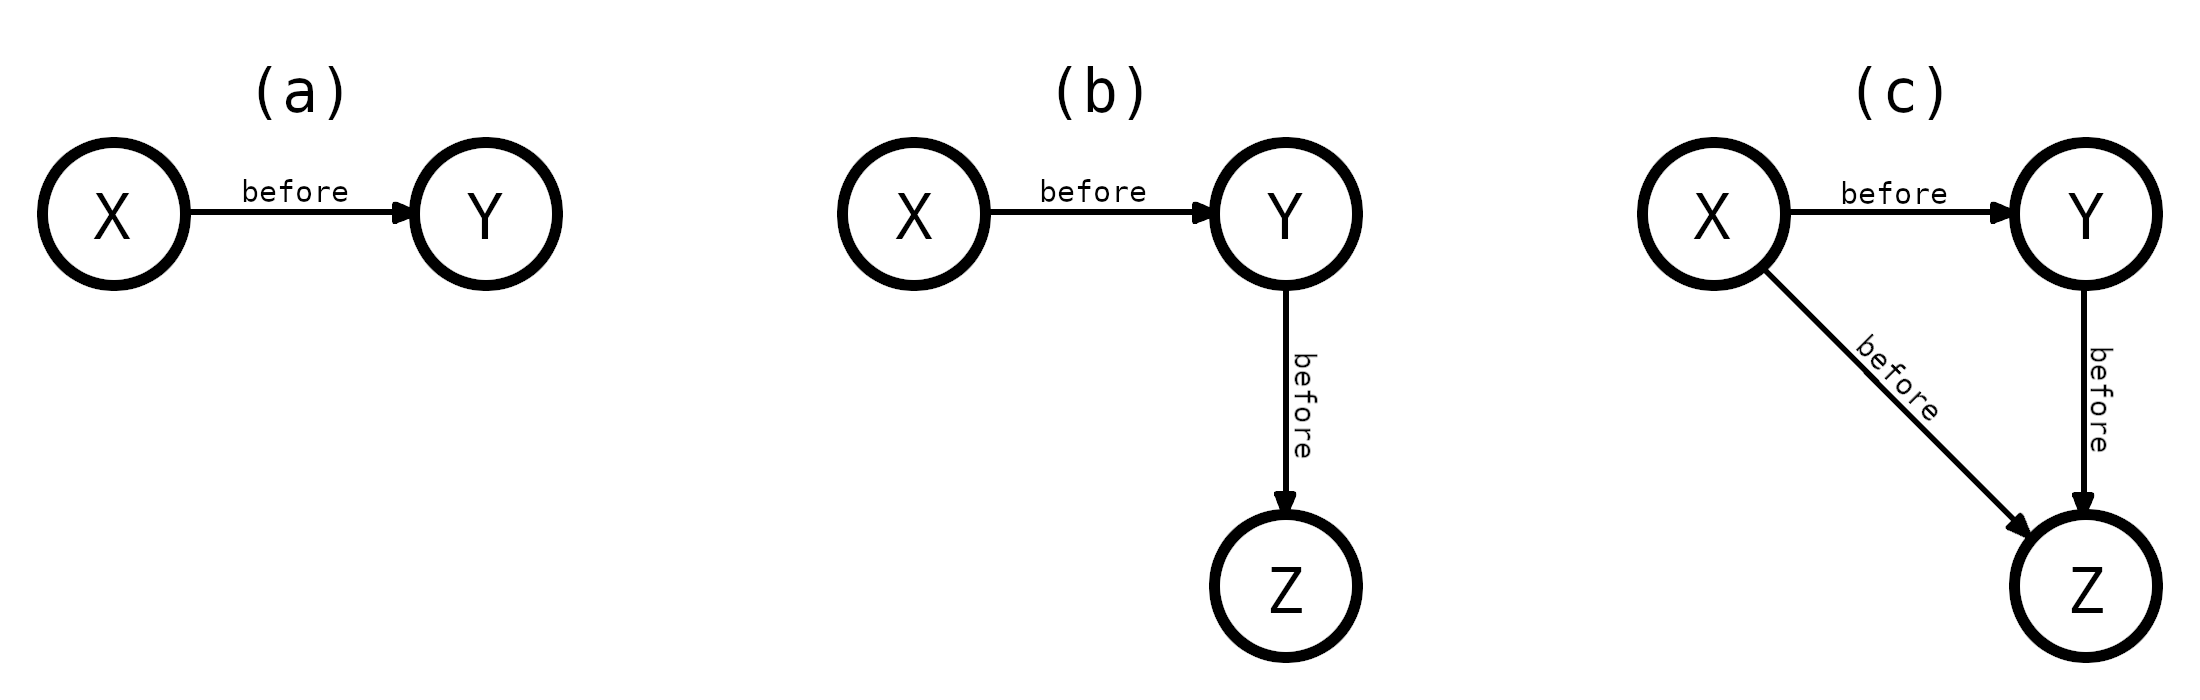
\includegraphics[width=\textwidth]{images/simple-transitivity}
		\captionof{figure}{Simple graph network showing the computation of a transitivity.}
		\label{fig:simple-transitivity}
	\end{figure}
\end{center}
For $N$ nodes (intervals) there are $\frac{N^2-N}{2}$ edges if all new nodes are connected to all existant nodes when they are created. While in \Cref{fig:simple-transitivity} there is one label per edge, there may be as many as $13 \cdot \frac{N^2-N}{2}$ labels per edge if there is no knowledge about any relations. In \Cref{fig:complex-transitivity}, it can be seen that a pair of single-label edges may result in a multiple-label edge by transitivity: the relations $X$ o $Y$ and $Y$ o $Z$ results in the disjunction of $X$ \textless $Z$, $X$ o $Z$, and $X$ m $Z$. Without further data, there is no way to definitively constrain this disjunction to a single relation. If there is a single label for every edge in the graph, this is known as \textit{temporal closure}---as discourse often naturally features incomplete or vague temporal information, calculating the temporal closure is, in general, a difficult goal to achieve, though it is desirable in order to create a representation that is both complete and consistent \citep{Verhagen2005}.
\begin{center}
	\begin{figure}[h!]
		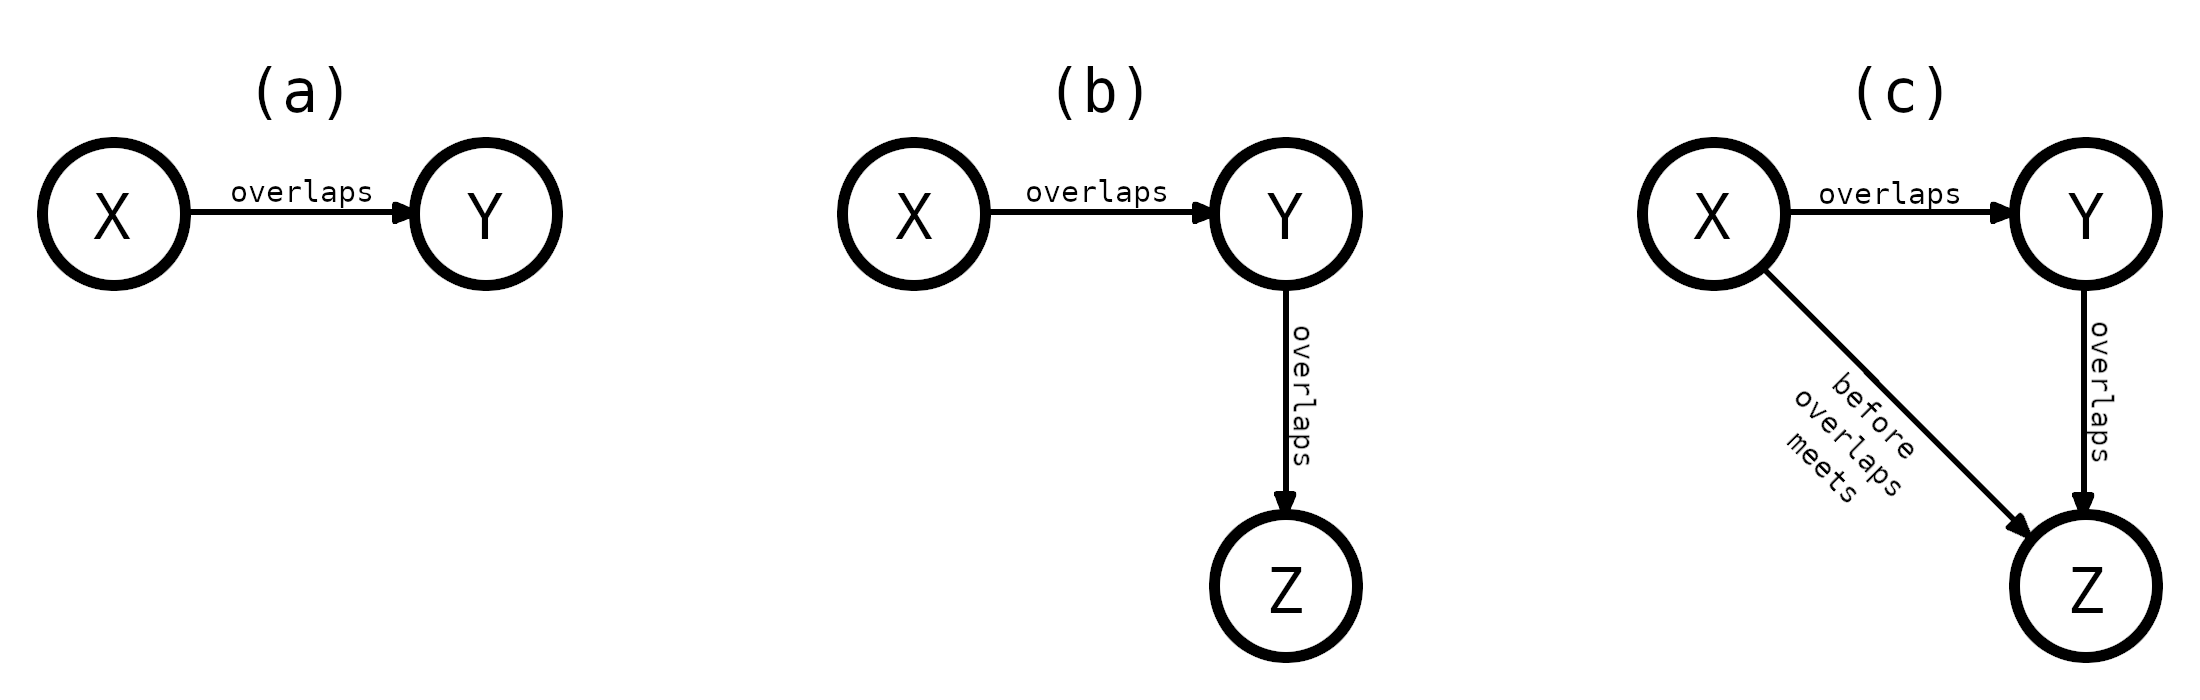
\includegraphics[width=\textwidth]{images/complex-transitivity}
		\captionof{figure}{Computation of a transitivity with a multiple-label result.}
		\label{fig:complex-transitivity}
	\end{figure}
\end{center}
\citet[p. 836]{allen1983maintaining} gives a $12 \times 12$\footnote{The equals relation is omitted, since it is reflexive, symmetric, and transitive, meaning for any relation $\bigcdot$, $((A = B \land B \bigcdot C) \lor (A \bigcdot B \land B = C)) \Longrightarrow A \bigcdot C$.} transitivity table---a $6 \times 6$ fragment of which is reproduced below in \Cref{tab:allen-trans-table}---which provides the relation or relations which may exist between two intervals $A$ and $C$, given the relations $\bigcdot$ between $A$ and $B$, and $\bigcdot'$ between $B$ and $C$. Not shown in \Cref{tab:allen-trans-table} are relation pairs such as $A$ before $B$ and $B$ after $C$---the disjunction of relations between $A$ and $C$ in this case contains all 13 possibilities (in Allen's table, labelled as `no info'), indicating that there are no constraints on the relation between $A$ and $C$. A smaller fragment of this table which shows these transitivities interpreted as superpositions\footnote{See \cref{ssub:operations} for details of superposition.} of strings which represent the various Allen relations is given in \citet[p. 130]{woods2017towards}. One advantage of the string-based approach comes from the fact that a single string may be used to represent an arbitrary (finite) number of events, and all of the relations between them, at once---thus transitivities between, for example, four intervals can be represented as easily as three.% \nb{Table of this somewhere?}

\begin{center}
	\onehalfspacing
	\begin{tabular}{|c|c|c|c|c|c|c|}
		\hline
		\diagbox{$A \bigcdot B$}{$B \bigcdot' C$} & \textbf{\textless{}} & \textbf{d} & \textbf{o} & \textbf{m} & \textbf{s} & \textbf{f}\\
		\hline
		before \textbf{(\textless{})} & \textless{} & \textless{} o m d s & \textless{} & \textless{} & \textless{} & \textless{} o m d s\\
		\hline
		during \textbf{(d)} & \textless{} & d & \textless{} o m d s & \textless{} & d & d\\
		\hline
		overlaps \textbf{(o)} & \textless{} & o d s & \textless{} o m & \textless{} & o & o d s\\
		\hline
		meets \textbf{(m)} & \textless{} & o d s & \textless{} & \textless{} & m & o d s\\
		\hline
		starts \textbf{(s)} & \textless{} & d & \textless{} o m & \textless{} & s & d\\
		\hline
		finishes \textbf{(f)} & \textless{} & d & o d s & m & d & f\\
		\hline
	\end{tabular}
	\captionof{table}{Fragment of Allen's transitivity table \citeyearpar[p. 836, Figure 4]{allen1983maintaining}.}
	\label{tab:allen-trans-table}
\end{center}
\label{other:allen-algo}For the propagation of constraints upon the addition of new information to the network, \citet[p. 835]{allen1983maintaining} also details an algorithm using the transitivity table to update all arcs in the network as necessary. While Allen does concede that there are some issues with this algorithm---specifically mentioning the space requirement, which is somewhat high at $O(N^2)$ space for $N$ temporal intervals, and the fact that the algorithm doesn't guarantee consistency in larger than three-node networks\footnote{See \cref{sub:applications}, p. \pageref{ex:str-inconsistency} for how this limit may be improved upon by using strings and superposition to automatically reject inconsistencies.}, and \citet[p. 219]{Verhagen2005} also notes an $O(N^3)$ time complexity---it does give an upper bound of $13 \times \frac{(N - 1)(N - 2)}{2}$ to the number of modifications that can be made to the network, regardless of the number of constraints added. Additionally, ``the average amount of work for each addition is essentially linear (i.e., $N$ additions take $O(N^2)$ time; one addition on average takes $O(N)$ time)'' \citep[p. 837]{allen1983maintaining}. This is still quite high, given that it is not unusual for a given text, annotated documents of the TimeBank \citep{pustejovsky2003timebank,pustejovsky2006timebank} corpus for instance, to feature fifty intervals or more, and some are in the hundreds \citep[p. 213]{Verhagen2005}.

To tackle the space requirements while maintaining as much inferential power as possible, \citet[p. 838]{allen1983maintaining} also describes a method for grouping clusters of intervals which---in regards to the relations between them---are fully computed, termed ``reference intervals''. This is due to the fact that each interval $I_i$ in the cluster $\{I_1, I_2, ..., I_n\}$ will reference one or more new intervals $R_m$ (where $m$ is an index on the number of reference intervals), and these reference intervals will be connected in the graph, which can be used to find relations between nodes which are not directly connected. Since these reference intervals may be treated as normal intervals, they may themselves be grouped into a cluster, and thus hierarchies of intervals may arise.% These are not currently implemented in the present work, but they may be useful as a way to address documents with high numbers of intervals.

Allen's work was and remains highly influential in the field of temporal reasoning and annotation, thanks to an approach which is both intuitive and straight-forward, as well as easy to implement in various applications. One such proponent of interval relations has been TimeML, a markup language designed to ``capture the richness of temporal and event related information in language'' \citep[p. 123]{Pustejovsky2005}---see \cref{ssub:timeml}.


\subsubsection{Tense and Aspect}\label{ssub:tenseaspect}
Reichenbach's (\citeyear{reichenbach1947elements}) theory of verbal tense and aspect allows for the temporal placement of an event time in relation to a speech time and a reference time. The relative orderings of these three times gives rise to the categorisations of tense and aspect in English and other languages. This framework has been widely accepted and adopted, and has found empirical validation via TimeML \citep{timeml2005timeml} and the TimeBank corpus \citep{pustejovsky2003timebank} in \citet{Derczynski2013}, which finds that using \citet{Freksa1992}'s semi-interval relations leads to ``tense appropriately constrain[ing] the types of temporal relations that can hold between pairs of events described by verbs''.
%While verbs are not the only expression of events, these categorisations can convey enough information to temporally locate that event

% \nb{Bring up TEA here somewhere. Also worth mentioning Vendler and Dowty in relation to lexically telic/atelic verbs, which inform the stative-based approach of the strings and thus block compression. Tim mentioned that this is a difference from Schwer's S-Words.}
% Reichenbach, Vendler, TEA
% Aspect hypothesis of dowty - build from statives - this is behind block compression/destuttering
% as difference for Schwer s-words

\citet[p. 72]{reichenbach1947elements} initially presents six tense/aspect combinations of English as arrangements of three temporal points, the `point of the event', the `point of reference', and the `point of speech', which may coincide. These six are: the Simple Past, Past Perfect, Present, Present Perfect, Simple Future, and Future Perfect. However, it is noted that the `Simple Future' may have two possible interpretations in English, and the arrangement originally presented under that name---where the points of speech and reference are equal and precede the point of the event---is later (p. 77) renamed as the `Posterior Present', while the second interpretation becomes the arrangement associated with the term `Simple Future'---see \Cref{fig:reichenbach-arrangements}.



% This is reproduced in \Cref{fig:reichenbach-arrangements} below, with $E$ for the event time, $R$ for the reference time, and $S$ for the speech time:

% \citet[p. 77]{Derczynski2013}: ``PERFECTIVE PROGRESSIVE aspect was converted to PERFECTIVE; this feature value accounts for 20 of 5974 verb events, or 0.34%''
\begin{center}
	\begin{tabular}{|l l c|}
		\hline
		\textbf{Tense} & \textbf{Example} & \textbf{E, R, S}\\
		\hline
		Simple Past & ``I bought the book'' & $(E = R) < S$\\
		Past Perfect & ``I had bought the book'' & $E < R < S$\\
		Simple Present & ``I buy the book'' & $E = R = S$\\
		Present Perfect & ``I have bought the book'' & $E < (R = S)$\\
		Simple Future & ``I will buy the book'' & $S < (R = E)$\\
		Future Perfect & ``I will have bought the book'' & $S < E < R$\\
		\hline
	\end{tabular}
	\captionof{figure}{Arrangements of the points $E$, $R$, and $S$, from \citet{reichenbach1947elements}.}
	\label{fig:reichenbach-arrangements}
\end{center}
As can be seen from these arrangements, the tense of a sentence being in the Past, Present, or Future tense correlates to the ordering of the reference time $R$ and speech time $S$: whether the reference time $R$ appears before, equal to, or after the speech time $S$, respectively. The perfective aspect---called the `Anterior' tenses in \citet[p. 77]{reichenbach1947elements}---is then created by placing the event time $E$ before $R$, where it is equal to $R$ in the non-perfective aspect.

While \citet{reichenbach1947elements} (mostly) treats the time of event, speech and reference as temporal points, there is so far no issue with assuming that they may instead be treated as temporal intervals, \`{a} la \citet{allen1983maintaining} and TimeML \citep{timeml2005timeml,sauri2006timeml}. However, in order to treat the Progressive aspect which English may use, the so-called `point of the event' must in fact be taken as an interval rather than an instantaneous point, indicating the durative nature of the Progressive. If the event time was already considered to be an interval, then instead the set of relations must change so as to include the `during' relation from Allen's set---see \Cref{fig:allens-pictorial}, p. \pageref{fig:allens-pictorial}. Thus the Progressive aspect can be conceptualised by the reference time $R$ occurring during the event time $E$, as in \Cref{fig:reichenbach-progressive}.
\begin{center}
	\begin{tabular}{|l l c|}
		\hline
		\textbf{Tense} & \textbf{Example} & \textbf{E, R, S}\\
		\hline
		Past Progressive & ``I was buying the book'' & $R ~d~ E,~ R < S$\\
		Present Progressive & ``I am buying the book'' & $R ~d~ E,~ R = S$\\
		Future Progressive & ``I will be buying the book'' & $R ~d~ E,~ S < R$\\
		\hline
	\end{tabular}
	\captionof{figure}{Relations of $E$, $R$, and $S$ for the Progressive aspect.}
	\label{fig:reichenbach-progressive}
\end{center}
However, if all of $E$, $R$, and $S$ are intervals, then Allen's interval relations apply to all pairings. Where before there was an equality relation between two of the points, Allen's equality will apply, but if one point preceded another, then in fact either of the `before' or `meets' relations may hold. Additionally, taking the Past Progressive as an example gives $R ~d~ E$ and $R < S$---assuming for the moment that $R$ is before $S$ rather than meeting it, then by the rules of transitivity for Allen relations, the relation between $E$ and $S$ may be any of `before', `meets', `contains', `finished by', or `overlaps'. The fact that these disjunctions arise leads \citet{Derczynski2013} to use \citet{Freksa1992}'s set of 31 semi-interval relations---a superset of Allen's interval relations---in validating the Reichenbachian framework within the TimeBank \citep{pustejovsky2006timebank} corpus. Semi-intervals arise by considering an interval in terms of its beginning and ending, but treating those as intervals in and of themselves, and in this way a set of relations are defined between the beginnings and endings of events. For instance, if the Freksa relation `older' holds between some pair of events $a$ and $b$, then the beginning of $a$, $\alpha(a)$, occurs before the beginning of $b$, $\alpha(b)$, while the order in which the events end is left unspecified. Each Freksa relation may also be described in terms of a disjunction of Allen relations---in fact, the `older' relation corresponds to the same disjunction of `before', `meets', `contains', `finished by', or `overlaps' which appear between a verb's event time $E$ and its speech time $S$ in the Past Progressive. The Freksa relations are discussed in more detail in \cref{ssub:incomplete}, but they are relevant here due to the disjunctions which come out of treating event, reference, and speech times as events, and leveraging shared reference times may lead to more of these disjunctions arriving when attempting to derive temporal relations between verbal events---see \Cref{fig:tense-aspect-freksa}.

By using what \citet[p. 74]{reichenbach1947elements} refers to as the ``permanence of the reference point'', events in an utterance may be temporally ordered relative to each other. This states that, though events may be in different clauses, the fact that a speaker adjusts the use of tense and aspect for the events relative to each other shows that they must share a reference time. In the following example \cref{ex:permanent-ref-pt}, the two events are in boldface.
\begin{itemize}
	\item[\ipp\label{ex:permanent-ref-pt}] ``I had \textbf{left} her when I \textbf{bought} the book.''
\end{itemize}
Since the two events are in the same utterance, they have the same speech time, and by permanence of reference point, their reference times are also identical. Now, given that `left' is in the Past Perfect, while `bought' is in the Simple Past, the constraints from \Cref{fig:reichenbach-arrangements} can be used to order the two events---using points rather than intervals for the sake of keeping the example simple---as follows in \cref{ex:permanent-ref}:

\begin{subequations}\label{ex:permanent-ref}
	\onehalfspacing
	\begin{align}
		S_{leave} = S_{buy},~ R_{leave} = R_{buy}\\
		E_{leave} ~<~ R_{leave} ~<~ S_{leave}\\
		E_{buy} = R_{buy} ~<~ S_{buy}\\
		\therefore~~~ E_{leave} ~<~ E_{buy}
	\end{align}
\end{subequations}
This gives that the event time of `left' $E_{leave}$ occurs before the event time of `bought' $E_{buy}$, and thus for any pair of verbal events $a$ and $b$ which share a speech and reference time and the verb denoting $a$ is in the Past Perfect while the verb denoting $b$ is in the Simple Past, we can deduce that $a$ precedes $b$, as temporal points. While this principle still holds when $E$, $R$, and $S$ are treated as intervals instead of points, it does become a little more complex as the size of the possible relation set between a pair of intervals is over four times larger than the possible relation set for points, and as mentioned above, it is possible for disjunctions of relations to arise. \citet{Derczynski2013} give a table with all of the combinations of tense \{\texttt{PAST}, \texttt{PRESENT}, \texttt{FUTURE}\} and aspect\footnote{The \texttt{PERFECTIVE\_PROGRESSIVE} aspect is also possible---for example in ``I had been walking''---however, it is omitted for simplicity's sake due to featuring in less than 1\% of verb events in the TimeBank corpus \citep[p. 77]{Derczynski2013}.} \{\texttt{NONE}, \texttt{PROGRESSIVE}, \texttt{PERFECTIVE}\}---the aspect value of \texttt{NONE} denotes the Simple form of that tense---where each disjunction has been labelled with its associated Freksa relation, displayed in \Cref{fig:tense-aspect-freksa}.
\begin{center}
	\begin{figure}[h!]
		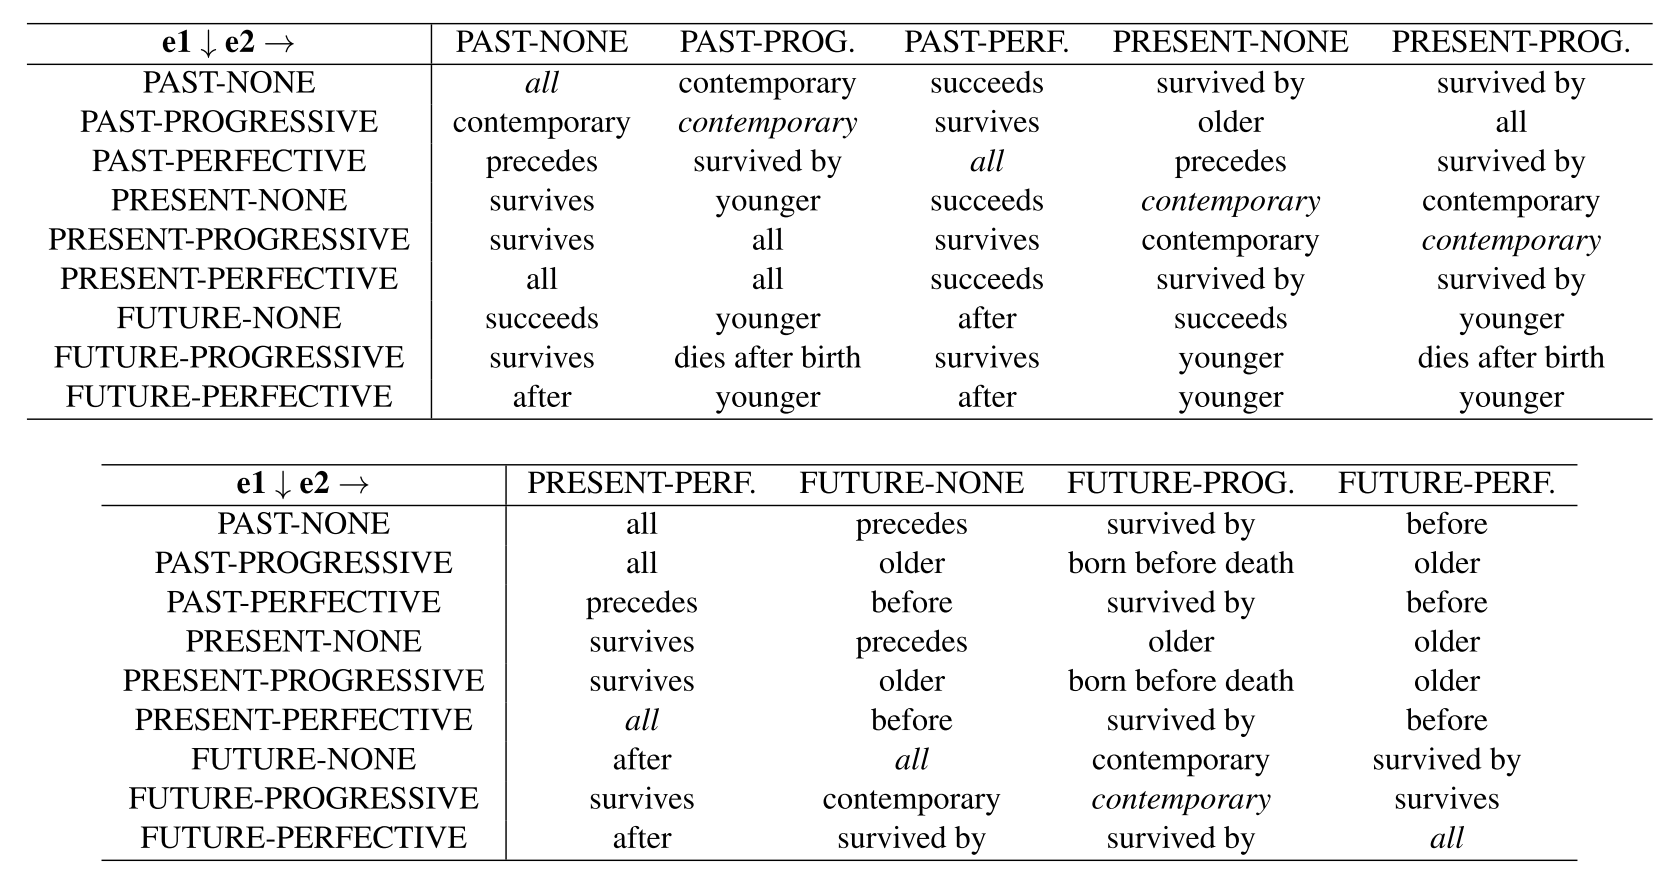
\includegraphics[width=\textwidth]{images/tense-aspect-freksa}
		\captionof{figure}{Tense-aspect pairs and the \citet{Freksa1992} relations they may suggest\\\citep[taken from][p. 80, Table 5]{Derczynski2013}.}\label{fig:tense-aspect-freksa}
	\end{figure}
\end{center}
Care must be given, though, to note that the rule of a permanent reference time only applies to verbs within the same \textit{temporal context} \citep{hornstein1990time,Derczynski2013}---verbs appearing in reported speech, for instance, are in a separate context to the verbs which introduce it. For example, in \cref{ex:reported-speech}, the events pointed to by `put' and `said' share their speech and reference times, and thus their temporal context is the same. However, `going' is part of a separate statement, enclosed by the quotation marks, and having a speech time that is equal to the event time of `said'.

\begin{itemize}
	\item[\ipp\label{ex:reported-speech}] He \textbf{put} his head in and \textbf{said} ``I'm \textbf{going} to the shop''.
\end{itemize}
In general, if a pair of events that are to be temporally related are in separate temporal contexts ``Reichenbach's framework may not directly apply, and the pair should not be further analysed'' \citep[p. 75]{Derczynski2013}. However, the temporal context can be difficult to determine automatically from a text, and the TimeML schema doesn't provide an explicit way to annotate it. One way to model a shared context between some pair of events is to look at the proximity of their appearance in the text, assuming events which are more textually distant than an adjacent sentence are unlikely to share the same context, and additionally checking if the events share the same tense---that is, the same speech and reference time. Using this model on the TimeBank 1.2 \citep{pustejovsky2006timebank} corpus, \citet[p. 80]{Derczynski2013} validated the Reichenbachian framework of tense and aspect by extracting pairs of verbal events from the \verb|<TLINK>| tags and using the tense and aspect of the verb pairs to derive one of the disjunctions of relations given in \Cref{fig:tense-aspect-freksa}. This derived disjunction contained as an element the relation that was actually marked up in the \verb|<TLINK>| tag in 67.8\% of cases\footnote{This excludes the prediction of the `all' or `unknown' relation, which is a disjunction of all possible relations. Including this relation is not useful, but when doing so the accuracy was found to be 91.9\%.}. It is noted that, taking into consideration that the temporal context model is somewhat crude, the amount of inaccuracy using this model (32.2\%) is comparable to the inter-annotator disagreement for \verb|<TLINK>| relation type labels (0.23) in the corpus: ``The fact that temporal context is derived from models and not explicit gold-standard annotation is also likely a significant source of noise in agreement.'' \citep[p. 80]{Derczynski2013}.

The next section takes a deeper look at the TimeBank corpus and the annotation schema with which it is marked up, TimeML.

\subsection{Temporal Annotation}\label{sub:annotation}
Ideally, humans who use artificially  intelligent systems for question-answering, scheduling, or other applications which require some level of reasoning about temporal data won't ever have to consider the annotation which drives it---except, of course, in the case when annotation is itself the goal of using the system. Computer systems have no inherent understanding of natural language, and rely on the samples they have been provided with in order to give a facsimile of the communication abilities that humans have. The better the quality of those samples, and the more information embedded within them, the better the system can interpret human language, and in turn generate interpretable output.

The annotation of a document allows for information about the text to be expressed in such a way as to make the implicit explicit---revealing a layer of semantics which a human may be able to infer, but an artificial agent would not. There are many ways to mark up a text, and many concepts which may warrant marking up, but in terms of temporal data, the most prudent schema to follow is that of TimeML \citep{timeml2005timeml} and its successor, which has become the ISO (International Organization for Standardization) standard for temporal annotation: ISO-TimeML \citep{ISO24617-1}, a part of the ISO Semantic Annotation Framework---see \citet{Bunt2020}.

% Derczinski
TimeML has found considerable success in terms of widespread adoption as a means of marking up text with temporal information, at least in some part thanks to the release of TimeBank \citep{pustejovsky2003timebank}, a corpus of newswire articles\footnote{The original version of TimeBank contained 300 articles, while the latest version, TimeBank 1.2, contains 183.} which were manually annotated using the TimeML schema. TimeBank frequently appears in discussion about TimeML since, in terms of quality, manual annotation is still seen as the `gold standard' and superior to automatically generated markup, although machine-created annotation has seen much effort and improvement in recent years \citep{mani2006machine,uzzaman2013semeval,reimers2016temporal}.

The availability of appropriate tooling for the creation of human-driven annotation is crucial in ensuring that accurate and consistent results are produced. The first edition of the TimeBank corpus was annotated using the Alembic Workbench tool \citep{day1997mixed}, which was useful for the non-relational aspects, but impractical for the highly relational nature of the temporal data featured in TimeML annotations \citep{verhagen2005TBOX}. A number of other tools have been developed since then which aim to provide visual feedback and assistance to an annotator, including using directed graphs---as in \citet{allen1983maintaining}---and timeline-like depictions, of which the tooling described in \cref{sec:implementation} falls under the second category.

\subsubsection{TimeML and TimeBank}\label{ssub:timeml}
The initial goal for creating the TimeML language came from a desire to improve applications\allowbreak{}---such as question-answering systems---by means of event recognition, and giving each recognised event an explicit temporal location. This latter point is motivated due to the fact that a large proportion of temporal information in discourse rely on implicit or vague temporal expressions. This relates back to the first principle which \citet{allen1983maintaining} mentioned\footnote{See p. \pageref{other:allen-motivations}.} as influencing the design of the interval algebra framework: that it is not generally intuitive to always think of or refer to time in terms of explicit or precise time points. Instead we tend to use relative expressions, such as the boldface text in the following utterances:
\begin{itemize}
	\item[\ipp] ``I didn't go to work \textbf{last Monday}.''
	\item[\ipp] ``I was sick \textbf{the week before}.''
\end{itemize}
Speakers will rely on their listeners being able to use context to interpret what these temporal expressions refer to.

TimeML aimed, in part, to give implicit and relative temporal expressions an explicit anchoring, in order to assist with  intelligent systems' temporal awareness. \citet[p. 125, (1a.)]{Pustejovsky2005} wanted to enable question-answering systems to be able to answer questions such as
\begin{itemize}
	\item[\ipp] ``Is Schr\"{o}der currently German chancellor?''
\end{itemize}
as capably as a human could after reading an appropriately relevant news article. A number of issues are raised that ought to be addressed within a system that can understand and answer questions similar to this one. Potentially problematic example queries can range from simple questions about the date of a specific event:
\begin{itemize}
	\item[\ipp] ``When did the USA first declare independence from the UK?''
\end{itemize}
to questions about non-unique events:
\begin{itemize}
	\item[\ipp] ``How long does it take to drive from Dublin to Cork?''
\end{itemize}
and questions where the system must perform some level of inference in order to derive the answer, possibly returning information that is not temporal in and of itself, but requires such data to find the correct solution:
\begin{itemize}
	\item[\ipp] ``Who was the last president of France?''
\end{itemize}
\citet[p. 132]{Pustejovsky2005} further discusses the kinds of temporal information that might be needed, and how to go about representing it in a useful way. Two tasks are deemed essential: the ability to place events on some timeline, and the ability to determine the relative order of any pair of events. These tasks are termed event \textit{anchoring} and \textit{ordering}, respectively, and these also form a core motivation for the framework described in \cref{sec:fst}, which uses strings to simultaneously represent the anchoring and ordering of events.  %a core part of the present work. Beyond these two tasks, the ability to identify and extract events and times from texts is an important task.

Events in TimeML are ``referred to by finite clauses, nonfinite clauses, nominalizations, event-referring nouns, adjectives, and even some kinds of adverbial clauses'' \citep[p. 133]{Pustejovsky2005}. Systems must also be aware of the possibility of negated and modal events, such as:
\begin{itemize}
	\item[\ipp] ``Ireland did \textbf{not} \textit{make it} to the World Cup this year.''
	\item[\ipp] ``The exhibition \textbf{might} \textit{create} new opportunities for the museum.''
\end{itemize}
The events (italicised) in these sentences should not be treated as if they actually occurred. Additionally, care should be taken to distinguish separate events in the representation which are referred to together in the text \citep[p. 134, (32a.)]{Pustejovsky2005}:
\begin{itemize}
	\item[\ipp\label{other:pustejovsky-type-instance}] ``James \textit{taught 3 times} on Tuesday.''
\end{itemize}
This leads to a distinction between types of events and instances of events, where an instance may appear in the representation in place of a type, \textit{cf.} \cref{ex:judder}, p. \pageref{ex:judder}.

Times, on the other hand, generally take the form of adverbial or prepositional phrases in English, such as `next week', `yesterday', or `10th of August'. For TimeML, these expressions must be normalised in order to anchor events to times on a timeline---converted to some machine-readable form, possibly an integer or real number, depending on the context. It is also important to know the time of utterance (or document creation time, for a text) in order to correctly normalise expressions such as `today' or `last Monday', as these terms refer to a time which is relative to some other point, often the time of utterance or document creation time. Some expressions, such as `recently' cannot be determinately linked to the timeline, due to their inherently vague nature, yet may still be ordered relative to other time points, and thus should still undergo normalisation. The last two kinds of time expressions mentioned in \citet{Pustejovsky2005} are durations and sets of times. Durations, such as `five hours', may or may not be anchored to times or events (boldface text):
\begin{itemize}
	\item[\ipp] ``You'll have it for \textit{a month} from \textbf{Monday}.''
	\item[\ipp] ``She submitted \textit{two weeks} before \textbf{the deadline}.''
\end{itemize}
Sets of times are generally used to place recurring events on the timeline:
\begin{itemize}
	\item[\ipp] ``He visited \textit{every week}.''
	\item[\ipp] ``They took the meds \textit{twice a day}.''
\end{itemize}
% 
% While the current work deals directly with data that is already annotated with markers for events and times, it is worth keeping this instructive material on extraction of temporal data in mind. The TimeBank corpus \citep{pustejovsky2006timebank} is a large collection of documents (in the domain of news articles) manually annotated with TimeML, and as such contains a number of human errors (e.g. inconsistencies in relation-labelling). It is also not as completely labelled as it could be, and has also not been updated in several years. It is conceivable, then, that an alternative source for data may at some point become desirable, either due to the release of a more attractive corpus, or by creating an entirely new corpus, following the same general principles as in TimeBank.
% 
In order for TimeML to represent the desired ordering and anchoring, a set of relations for times and events is required, and Allen's interval relations are selected as a strong basis for these, as reasoning over them is ``well-understood'' \citep[p. 138]{Pustejovsky2005}. However, it is noted that not all of Allen's relations are equally well represented in texts of the English language. In particular, the \textit{overlaps} relation is ``difficult to find instantiated in natural language text'', and thus may be considered unnecessary. In fact, this relation and its inverse are omitted from the final set of temporal relations used in TimeML---see \Cref{fig:tlink-allen-translation}. Nevertheless, since these relations may arise through transitivity and it is not immediately problematic to do so, they are reincluded in \cref{sec:implementation}.

The syntax of TimeML\footnote{For the full specification of TimeML (version 1.2.1), see \url{http://www.timeml.org} \citep{timeml2005timeml}, and annotation guidelines in \citet{sauri2006timeml}.} % \url{https://www.cs.brandeis.edu/~cs112/cs112-2004/annPS/TimeML12wp.htm} \citeneeded{}
uses the following types of tags to capture the various kinds of information: \verb|<TIMEX3>| for marking up time expressions, \verb|<EVENT>| for events and \verb|<MAKEINSTANCE>| for event instances, \verb|<SIGNAL>| for functional words (such as `at', `from', `when', etc.), and three types of linking tags for relations between the other tags: \verb|<SLINK>| captures subordinating relations involving evidentiality, modality, and factuality; \verb|<ALINK>| captures aspectual links; and \verb|<TLINK>| captures temporal relationships between events and times.

\Cref{ssub:tlinks,sec:implementation} focus primarily on this last tag type, as it is here that Allen's interval relations are represented, albeit under slightly different nomenclature, with some duplication, and omitting the overlapping relations as mentioned above---see \Cref{fig:tlink-allen-translation}. Each of TimeML's tags take a number of attributes which help to flesh out the representation of the information, and for a \verb|<TLINK>| these are: either a \texttt{timeID} or \texttt{event\allowbreak{}InstanceID}, which refers to some temporal expression in the text; either a \texttt{relatedTo\allowbreak{}Time} or \texttt{relatedTo\allowbreak{}Event\allowbreak{}Instance}, which will refer to another temporal expression; and a \texttt{relType}, which will specify the relation from the first attribute to the second.
\begin{center}
	\setstretch{1.15}
	\begin{tabular}[h!]{|c c|}
		\hline
		\textbf{TLINK} & \textbf{Allen}\\
		\hline
		\texttt{SIMULTANEOUS} & equal \textbf{(=)}\\
		\texttt{IDENTITY} & equal \textbf{(=)}\\
		\texttt{BEFORE} & before \textbf{(\textless{})}\\
		\texttt{AFTER} & after \textbf{(\textgreater{})}\\
		\texttt{IBEFORE} & meets \textbf{(m)}\\
		\texttt{IAFTER} & met by \textbf{(mi)}\\
		\texttt{INCLUDES} & contains \textbf{(di)}\\
		\texttt{IS\_INCLUDED} & during \textbf{(d)}\\
		\texttt{DURING} & during \textbf{(d)}\\
		\texttt{DURING\_INV} & contains \textbf{(di)}\\
		\texttt{BEGINS} & starts \textbf{(s)}\\
		\texttt{BEGUN\_BY} & started by \textbf{(si)}\\
		\texttt{ENDS} & finshes \textbf{(f)}\\
		\texttt{ENDED\_BY} & finished by \textbf{(fi)}\\
		\hline
	\end{tabular}
	\captionof{figure}{Possible values of a TLINK's relType attribute and their Allen relation counterparts.}\label{fig:tlink-allen-translation}
\end{center}
The rationale behind distinguishing \texttt{INCLUDES}/\texttt{IS\_INCLUDED} and \texttt{DURING\_INV}/\texttt{DURING} is that the former should be used for cases where an event or time is included in another, like in:
\begin{itemize}
	\item[\ipp] ``He \textbf{arrived} there \textbf{last week}.''
\end{itemize}
while the latter should be used specifically for states or events that persist throughout a duration \citep[p. 158]{Pustejovsky2005}, such as in:
\begin{itemize}
	\item[\ipp] ``They \textbf{were Captain} for \textbf{two seasons}.''
\end{itemize}
Below in \Cref{fig:example-timeml-annotation} is a simple example of a completed annotation---derived from the annotation guidelines \citep{sauri2006timeml}---of the sentence:
\begin{itemize}
	\item[\ipp] ``He panicked on Wednesday.''
\end{itemize}
\begin{center}
	\onehalfspacing
	\begin{tabular}[h!]{|l|}
		\hline
		\begin{minipage}{0.75\textwidth}
		\begin{verbatim}

		He
		<EVENT eid="e1" class="OCCURRENCE">
		 panicked
		</EVENT>
		<SIGNAL sid="s1">
		 on
		</SIGNAL>
		<TIMEX3 tid="t1" type="DATE">
		 Wednesday
		</TIMEX3>
		<MAKEINSTANCE eiid="ei1" eventID="e1" pos="VERB"
			tense="PAST" aspect="NONE" polarity="POS" />
		<TLINK eventInstanceID="ei1" relatedToTime="t1"
			signalID="s1" relType="IS_INCLUDED" />

		\end{verbatim}
		\end{minipage}\\
		\hline
	\end{tabular}
	\captionof{figure}{Example TimeML annotation for ``He panicked on Wednesday.''}\label{fig:example-timeml-annotation}
\end{center}
Since the initial publication of \citet{pustejovsky2003timeml}\footnote{In this work, the authors do refer to the TimeML language as being ``developed in the context of a six-month workshop, TERQAS'' during 2002. However, the URL link cited for \textit{Annotation Guideline to TimeML 1.0} (\url{http://time2002.org}) no longer available points to an available resource as of March 2021. The TERQAS (Time and Event Recognition for Question Answering Systems) workshop was held at MITRE Bedford and Brandeis University \citep[p. 647]{pustejovsky2003timebank}.}, TimeML has received numerous improvements, updates, and tweaks. Although a version of the language has been adopted as an ISO standard (ISO 24617-1:2012) for temporal annotation \citep{pustejovsky2010iso}, the most recent publically available version---see \url{http://www.timeml.org}---is TimeML 1.2.1 \citep{timeml2005timeml,sauri2006timeml}, and this is the version which the present work will focus on. The primary reason for this is due to the most recently available edition\footnote{This refers to the English language corpus. There do exist versions of other TimeBank corpora in languages such as French \citep{bittar2011french} and Hindi \citep{goel2020hindi} which use the ISO-TimeML schema.} of the TimeBank corpus---one of the largest available corpora for documents annotated with TimeML---being TimeBank 1.2 \citep{pustejovsky2006timebank}, wherein the annotation was updated in order to bring the corpus in line with the updated specification, which at the time was TimeML 1.2.1.

The TimeBank 1.2 corpus contains 183 texts, featuring news articles from a variety of sources, including broadcast news from ABC, CNN, PRI, and VOA, as well as articles from the Wall Street Journal. The counts for how frequently each tag appears in the corpus are given below in \Cref{fig:timebank-stats}, reproduced from \citet{pustejovsky2006timebank}:
\begin{center}
	\onehalfspacing
	\begin{tabular}[h!]{|l l|}
		\hline
		\textbf{Tag} & \textbf{Count}\\
		\hline
		EVENT & 7,935\\
		MAKEINSTANCE & 7,940\\
		TIMEX3 & 1,414\\
		SIGNAL & 688\\
		ALINK & 265\\
		SLINK & 2,932\\
		TLINK & 6,418\\
		% \hline
		\textit{Total} & 27,592\\
		\hline
	\end{tabular}
	\captionof{figure}{Tag counts for TimeBank 1.2.}\label{fig:timebank-stats}
\end{center}
The TempEval-3 \citep{uzzaman2013semeval} shared task, which aimed to ``advance research on temporal information processing'', also produced a slightly updated version of the TimeBank 1.2 corpus, which is described as having been ``cleaned''. This included adjusting all of the files to have consistent formatting, to be XML and TimeML schema compatible, as well as adding some missing events, times, and relations \citep[p. 2]{uzzaman2013semeval}.

While this work will focus on TimeML 1.2.1, it is worth outlining some of the most notable alterations which were introduced by ISO-TimeML. One of the largest changes, from a structural point of view, is moving away from in-line annotation, whereby the markup tags are inserted directly into the body of the text. Instead, ISO-TimeML separates the annotation from the main text, using ``stand-off'' annotation, which increases the interoperability of annotation languages by conforming to the general practice of not modifying the text which is being annotated \citep[p. 395]{pustejovsky2010iso}. For example, a sentence like in \cref{ex:inline-tag-sentence} which features an event that appears partway through will be marked up as something similar to \cref{ex:inline-tag-markup} (omitting some attributes) using the older versions of TimeML:
\begin{itemize}
	\item[\ipp\label{ex:inline-tag-sentence}] ``He walked to the shop.''
	\item[\ipp\label{ex:inline-tag-markup}] \verb|He <EVENT eid="e1" ... >walked</EVENT> to the shop.|
\end{itemize}
while ISO-TimeML would be something more like in \cref{ex:standoff-event-seg,ex:standoff-event-tml}, which are each in separate files:
\begin{itemize}
	\item[\ipp\label{ex:standoff-event-seg}] \verb|<seg type="token" xml:id="token1">He</seg>|\\\verb|<seg type="token" xml:id="token2">walked</seg>|\\\verb|<seg type="token" xml:id="token3">to</seg>|\\\verb|<seg type="token" xml:id="token4">the</seg>|\\\verb|<seg type="token" xml:id="token5">shop</seg>|
	\item[\ipp\label{ex:standoff-event-tml}] \verb|<EVENT xml:id="e1" target="#token2" ... />|
\end{itemize}
Additionally, the \verb|<EVENT>| tag is now explicitly used to denote an event instance, and as a result, the \verb|<MAKEINSTANCE>| tag no longer exists. Some of its attributes are shifted to the \verb|<EVENT>| tag, and \verb|<TLINK>| tags in ISO-TimeML use \texttt{eventID} and \texttt{relatedToEvent} instead of \texttt{eventInstanceID} and \texttt{relatedToEventInstance}, respectively.

\label{other:iso-mlink}Finally, ISO-TimeML also takes a proposal from \citep{bunt2010annotating} and provides a new type of link tag, \verb|<MLINK>|, which has an ``inherent relation type of \verb|MEASURE|'' \citep[p. 396]{pustejovsky2010iso}, and is used to better reflect the relationships between durative events and stretches of time---for instance, where an event may have been interrupted and resumed during some period, but is referred to as having taken the entire span of time. The new tag uses a measuring function \citep{bunt1985mass} to interpret the relation, so that period of time that is measured is equal to the sum of all of the spans of time that make it up, whether contiguous or not. For example, in the sentence:
\begin{itemize}
	\item[\ipp] ``It rained for an hour.''
\end{itemize}
it may not have been raining consistently for the full hour---there may have been a period of, say, twenty minutes when it abated---but it is valid to interpret it either as a full, non-stop hour of rain, or as a span of an hour during which it rained. This is what the \verb|<MLINK>| is designed to treat, as in the example \cref{ex:mlink} below (where \textit{P1H} refers to a period of 1 hour):
\begin{itemize}
	\item[\ipp\label{ex:mlink}] \verb|<EVENT xml:id="e1" pred="RAIN" />|\\\verb|<TIMEX3 xml:id="t2" type="DURATION" value="P1H" />|\\\verb|<MLINK eventID="e1" relatedToTime="t2" />|
\end{itemize}
ISO-TimeML introduces a number of other changes over TimeML, such as the alteration and addition of several tag attributes, with the general aim of increasing interoperability, making it easier for other systems or software that might make use of the represented information. However, neither version of the language is intended to stand truly alone, but rather annotations are created for use in other applications. As such, there is no built-in way to visualise the depicted timeline of times and events, which is an intuitive way\footnote{See \cref{ssub:timelines}.} to assist in understanding the anchoring and ordering of the temporal entities. As such---like the string-based framework described in \cref{sec:fst}---other tools have been created which aim to aid in this arena, either simply for visualising a completed annotation, or as means of assisting an annotator in creating the markup.

\subsubsection{Tango and T-BOX}\label{ssub:tango-tbox}
Manual annotation of temporal data in text is not a simple task, requiring a solid understanding of the annotation schema, a strong ability to identify and keep track of multiple times and events, as well as being skilled in interpreting the often vague temporal data that exists in language \citep[pp. 213--214]{Verhagen2005}. Accordingly, a number of tools have been designed with the aim of assisting an annotator in making more correct decisions, either by helping to visualise the temporal structure of the document, or by automatically computing relations or marking inconsistencies as the annotator works. For example, Tango \citep{pustejovsky2003tango} was developed with the aim of improving the annotation of documents with TimeML by allowing users to---quite literally---draw connections between times and events which were displayed graphically, as in \Cref{fig:tango}.
\begin{center}
	\begin{figure}[h]
		\centering
		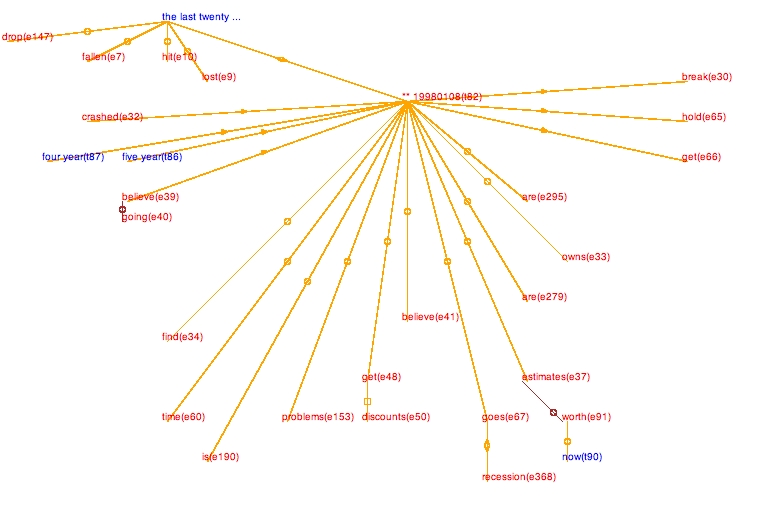
\includegraphics[width=0.9\textwidth]{images/tango}
	\end{figure}
	\captionof{figure}{Tango's interface \citep[taken from][p. 2, Figure 1]{verhagen2005TBOX}.}
	\label{fig:tango}
\end{center}
The graph here works on the same principle as those described in \cref{ssub:allen}, in that the nodes represent the events and times which are marked up in the TimeML document, while the arcs are labelled with the relation between the intervals. According to \citet[p. 2]{verhagen2005TBOX}, using Tango improved the quality and reliability of the annotations being produced, with a higher number of links being found between the nodes, though he also notes that Tango's main flaw is that it does not allow a user to ``quickly capture the temporal structure of the document'' \citep[p. 2]{verhagen2005TBOX}---that is, interpreting the overall chronology of a text by means of a directed graph is not straightforward for a human user of the technology. Part of the problem, according to \citet{verhagen2005TBOX}, is that the graph labels---representing the \verb|<TLINK>| tags of TimeML---quickly become difficult to read, especially when the document contains a large number of nodes. More troublesome, however, is the fact that there is no inherent semantics to the placement of the nodes; there is no graphical depiction of the temporal ordering, left-to-right or otherwise, that is enforced by the system in a meaningful way.

As a means of addressing some of these issues with the Tango tooling and its predecessor, the Alembic Workbench \citep{day1997mixed}, \citet{verhagen2005TBOX} presents the T-BOX framework, intended to be used in a complementary fashion alongside the table-based and graph-based depictions in the existant tools. T-BOX is based around the core idea that ``relative placement of two events or times is completely determined by the temporal relations between them'' (p. 2). The image shown in \Cref{fig:tbox} represents the same data as in \Cref{fig:tango}, placing each event and time into boxes (called T-BOXes), and using arrows, stacking, and box inclusion to represent the various relations between the temporal expressions that may be derived from \verb|<TLINK>| tags, under the assumption that events and times are intervalic, as described in \cref{ssub:allen}.

The rules governing placement of boxes are \citep[pp. 3--5]{verhagen2005TBOX}:
\begin{itemize}
	\item An event which occurs \textit{before} another is placed to the left of it, with an arrow leading from the one to the other, or a line ending in a dot if the relation is \textit{meets}.
	\item Simultaneous events are stacked, one box atop the other. Identical events are placed in the same box, rather than being treated the same as simultaneous ones.
	\item An event which \textit{contains} or \textit{includes} another gains an extended box with thinner walls, and the included event's box is placed inside this box.
	\item If an event \textit{starts} or \textit{finishes} another, it is placed inside that event's extended box, touching the left or right edge, respectively.
	\item Otherwise, none of these configurations may occur.
\end{itemize}

\begin{center}
	\begin{figure}[h!]
		\centering
		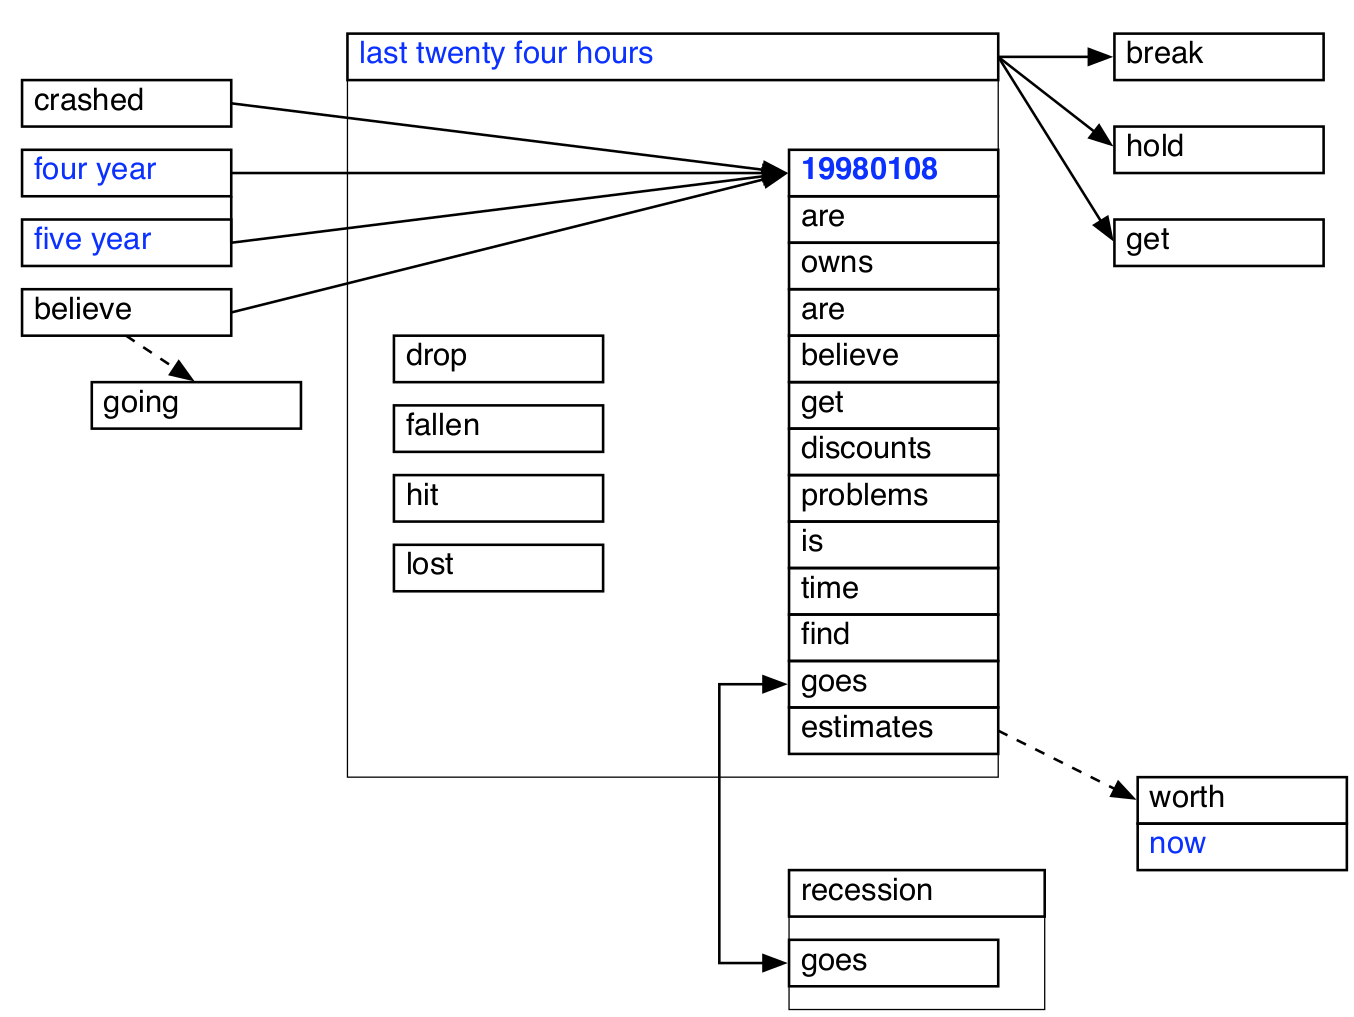
\includegraphics[width=0.8\textwidth]{images/tbox}
		\captionof{figure}{\Cref{fig:tango}'s data now drawn using T-BOX \citep[taken from][p. 3, Figure 2]{verhagen2005TBOX}.}\label{fig:tbox}
	\end{figure}
\end{center}
It is stressed that the vertical and horizontal positioning of boxes doesn't mean anything in and of itself, and thus despite a focus on semantically arranging and depicting the temporal relations in a TimeML annotation, T-BOX abandons the ``timeline metaphor'' \citep{verhagen2005TBOX}. However, using the string-based framework described in \cref{sub:strings}, many of the principles which guide the T-BOX architecture can be maintained whilst also preserving the ideology of timelines, being an intuitive way to conceptualise sequences of events and times---see \cref{ssub:timelines}.

Another point of interest with T-BOX is that it requires as input a TimeML document which is `complete', and has already had temporal closure constraints applied to its \verb|<TLINK>| tags, providing all of the inferrable relations ahead of time. It then reduces this to a minimal graph \citep[p. 6]{verhagen2005TBOX}. This is as opposed to the more typical scenario of trying to compute the temporal closure of a document using a constraint propogation algorithm---such as \citet{allen1983maintaining}'s in \cref{other:allen-algo}, p. \pageref{other:allen-algo}---or, as in the present work, using the superposition of strings to calculate relations at the same time as depicting them.

One further aspect of the T-BOX framework worth noting is that it can be used to possibly detect some inconsistencies in input data if there is some part of the data which cannot be drawn using the rules described above. For example, if the \verb|<TLINK>| tags give that some event X is \textit{before} some other event Y, that Y is \textit{before} a third event Z, and also that Z is \textit{before} X---an impossibility due to the circular transitivity---the inconsistency should be discovered when attempting to draw X to the left of Y, which is to the left of Z, which should then somehow be drawn to the left of X. However, while `non-drawability' implies an inconsistency, drawability does not imply consistency \citep[p. 12]{verhagen2005TBOX}, since similarly to the constraint propogation algorithm in \citet{allen1983maintaining}, inconsistencies may appear in the graph which appear consistent when looking at three intervals, but become problematic in a larger context. This issue can be circumvented using a string which may represent far more than three intervals and their relations at once, and strings which represent information inconsistent with the knowledge base are ejected through superposition---see \cref{def:vc-superposition}, p. \pageref{def:vc-superposition}---and thus, `non-superposability' can be seen as similar to the `non-drawability' of T-BOX.

The next section discusses some of the existing approaches to semantic representation of times and events aside from the semantics associated with the annotation schemas of TimeML and ISO-TimeML, in particular the structures of Discourse Representation Theory.

\subsection{Temporal Semantics of DRT}\label{sub:semantics}
% The following sections describe some of the existing ways that the semantics of times and events can be represented.
% \nb{This section needs more---Prior's TL, FOL, SOL, Event Calculus?, Frames?, Otherwise just make 2.3 about DRT... :/}
% \nb{Bunt (2020) mentions that Abziande \& Bos (2019) mention that almost everyone uses Neo-Davidsonian event semantics...}
% \nb{Harry Bunt's slides from his DCLRS talk would be useful here, else ref ``A semantic annotation scheme for quantification" (Bunt, 2019)}

% \subsubsection{Discourse Representation Theory}
In what have become robust and well-known works since their publication, \citet{kamp1981theory,kamp1988discourse,Kamp1993} presented Discourse Representation Theory (DRT) as a formal framework for semantically representing information derived from discourse---that is, coherent series of sentences or propositions, which may appear in speech or text. The development of DRT aimed to allow model-theoretic semantic representations that go beyond single sentences, which was the standard approach in First-Order Logic (FOL), and to treat phenomena such as anaphora, where an entity named earlier in a discourse may be referred to again later without naming it again. The classic example sentences \citep{kamp1988discourse} involve an indefinite, `a donkey', appearing as an antecedent, and acting as a quantifier which binds the pronoun `it' in the second sentence, as in \cref{ex:donkey-1}.
\begin{subequations}
	\begin{align}
		&\text{``John owns a donkey. He feeds it.''}\label{ex:donkey-1}\\
		&\exists x ~(donkey(x) \land own(John, x) \land feed(John, x))\label{ex:donkey-1-fol}
	\end{align}
\end{subequations}
The sentence in \cref{ex:donkey-2} is problematic in Montague-style approaches, which assume that any indefinite in a sentence should introduce an existential quantifier, but this comes into conflict with the scope of the universal quantifier introduced by `Every' \citep[p, 91]{kamp1988discourse}. In \cref{ex:donkey-2-fol}, the expected existential has acquired a universal force to capture the natural interpretation of \cref{ex:donkey-2} as claiming that every farmer feeds every donkey they own.
\begin{subequations}
	\begin{align}
		&\text{``Every farmer who owns a donkey feeds it.''}\label{ex:donkey-2}\\
		&\forall x \forall y ~((farmer(x) \land donkey(y) \land own(x,y)) \Longrightarrow feed(x,y))\label{ex:donkey-2-fol}
	\end{align}
\end{subequations}
DRT solves these issues with the notion of discourse referents, which are the set of entities under discussion in a given discourse, corresponding to the individual variables of FOL \citep[p. 397]{Bird2009}. Under DRT, indefinites do not introduce existential quantifiers, instead introducing new discourse referents, which are added to a mental representation known as a Discourse Representation Structure (DRS) \citep{geurts2007discourse}. DRSs contain separately both the discourse referents and the DRS conditions, which describe what is known about the referents. Multiple DRSs can be concatenated where it is appropriate to do so, with the result being a merged DRS containing the union of the discourse referents and DRS conditions from each of in the inputs to the concatenation \citep[p. 399]{Bird2009}.

For the example in \cref{ex:donkey-1}, the first sentence is processed and the two entities create two discourse referents, $x$ and $y$, which appear at the top of the DRS in \cref{ex:donkey-1-drs-a}, with the DRS conditions over these referents appearing in the lower box of the DRS.
\begin{align}
	\drs{$x~~~y$}{John($x$)\\donkey($y$)\\owns($x, y$)}\label{ex:donkey-1-drs-a}
\end{align}
As the second sentence of \cref{ex:donkey-1} is processed, the DRS is augmented with two further discourse referents, $u$ and $v$, corresponding with the two pronouns `He' and `it'. Resolving the anaphora\footnote{The component which performs the anaphora resolution is assumed separate to DRT, which merely sets constraints on which discourse referents are available as candidates for selection \citep[p. 399]{Bird2009}.} adds two new conditions, identifying the two pronoun referents with the two existing noun referents in \cref{ex:donkey-1-drs-a}. Finally the condition that $u$ feeds $v$ is added, giving \cref{ex:donkey-1-drs-b}.
\begin{align}
	\drs{$x~~y~~u~~v$}{John($x$)\\donkey($y$)\\owns($x, y$)\\$u = x$\\$v = y$\\feeds($u, v$)}\label{ex:donkey-1-drs-b}
\end{align}
There is a direct translation from a DRS to a formula of FOL, where the discourse referents which appear at the outermost level are interpreted as existential quantifiers, and the DRS conditions are interpreted as being conjoined. The translated formula for \cref{ex:donkey-1-drs-b} is in \cref{ex:donkey-1-drs-b-fol}, which has the same interpretation as \cref{ex:donkey-1-fol} despite its differences.
\begin{align}
	\exists x \exists y \exists u \exists v ~(john(x) \land donkey(y) \land owns(x,y) \land u = x \land v = y \land feeds(u, v))\label{ex:donkey-1-drs-b-fol}
\end{align}
Universal quantification is usually handled by embedding two DRSs connected by an implication within another DRS \citep[p. 98]{kamp1988discourse}, or alternatively by embedding a negated DRS within another embedded negated DRS\footnote{Due to the equivalence $\forall x~(P(x)) \Longleftrightarrow \lnot \exists x ~(\lnot P(x))$, stating that if some property $P(x)$ holds for all values of $x$, then there is no value for $x$ where $P(x)$ does not hold.}. Below, \cref{ex:donkey-2-drs} represents \cref{ex:donkey-2}.
\begin{align}
	\drs{$x$}{farmer($x$)\\\drs{$y$}{donkey($y$)\\owns($x,y$)} $\Longrightarrow$ \drs{$u$}{$u = y$\\feeds($x,y$)}}\label{ex:donkey-2-drs}
\end{align}
DRT is capable of representing events and times as temporal entities which introduce discourse referents and may appear in DRS conditions. For example, including a special `indexical' discourse refererent $now$ for the time of the utterance, as in \citet[p. 104]{kamp1988discourse} and \citet{abzianidze2017parallel}, \cref{ex:drs-temporal-b} represents the sentence in \cref{ex:drs-temporal-a}.
\begin{subequations}
	\begin{align}
		\text{``The doctor cured the patient.''}\label{ex:drs-temporal-a}\\
		\drs{$x~~y~~e~~now$}{doctor($x$)\\patient($y$)\\cure($e,x,y$)\\$e \prec now$}\label{ex:drs-temporal-b}
	\end{align}
\end{subequations}
The condition $e \prec now$ denotes that the event $e$ precedes the time of the utterance, indicating the past tense of the verbal event `cure'. Other temporal relations available in DRS conditions usually include $=$ equality, $\subset$ during, and $\bigcirc$ overlaps, though other relations occasionally are used, and in principle any binary relation could be used, including those in \citet{allen1983maintaining}'s set. It is possible in general to extract these relations and the events they refer to in order to build temporal-focused representations, such as the strings described in \cref{sec:fst}.

The DRS in \cref{ex:drs-temporal-b} represents a Davidsonian approach to event semantics, where an event variable $e$ was added as an argument to the predicate corresponding to the verb \citep{davidson1967logical,Kamp1993}, and DRSs can also feature discourse referents representing statives as well as eventives \citep[p. 103]{kamp1988discourse}. However, by introducing an event's semantic roles as conditions to the DRS, a neo-Davidsonian style \citep{dowty1989semantic} can be implemented instead, reducing the verbal predicate's arguments to just the event variable $e$. This is an approach which \citet{abzianidze2019thirty,Bunt2020} point out is the \textit{de facto} standard approach taken by most (if not all) semantically annotated corpora. Indeed, the Parallel Meaning Bank\footnote{Available at \url{https://pmb.let.rug.nl/}.} (PMB) corpus \citep{abzianidze2017parallel}---which aims to ``provide fine-grained meaning representations for words, sentences and texts'' and contains over 8000 DRSs from English sentences---uses this approach in their DRS representations. The DRS in \cref{ex:drs-temporal-c} below represents the sentence in \cref{ex:drs-temporal-a} again, this time including such semantic roles as might appear in the PMB, which uses an inventory of roles from the VerbNet resource \citep{schuler2005verbnet}.
\begin{align}
	\drs{$x~~y~~e~~now$}{doctor($x$)\\patient($y$)\\cure($e$)\\Agent($x$)\\Patient($y$)\\$e \prec now$}\label{ex:drs-temporal-c}
\end{align}
Automatic parsing of discourse text to DRSs is a non-trivial, multi-faceted task, involving tokenisation, part-of-speech recognition, and syntactic parsing before DRSs can even be constructed. A wide-coverage parser called Boxer was released by \citet{Bos2008}, which claimed 95\% converage for semantic analysis of newswire texts, although significantly for the present work, it was noted in that release that performance for temporal information was not as strong as its other areas \citep[pp. 283--285]{Bos2008}. Boxer takes as input a Combinatory Categorial Grammar (CCG) \citep{steedman2000syntactic,steedman2011combinatory} which has itself been parsed following named-entity recognition, and part-of-speech tagging prior to that, using the C\&C tools \citep{curran2007linguistically}, and outputs one or more DRSs as formally interpretable semantic representations \citep[p. 285]{Bos2008}. An updated version of Boxer \citep{van-noord-etal-2018-exploring} is implemented as part of the Parallel Meaning Bank toolchain \citep{abzianidze2017parallel}---although, this version had unfortunately not been made available for general use at the time of writing. However, the recent shared task created by \citep{abzianidze2019first} shows that there is an interest in developing systems which can perform automatic DRS parsing. The state-of-the-art was improved considerably in this task, with the winning system of \citet{liu2019discourse} achieving an F1 score of 84.8\%, an improvement from the baseline score of 54.3\%.

% One issue with DRSs in terms of representation for times and events

This chapter has attempted to give a general overview of some of the literature which informs the current work. In particular, the interval algebra put forward in \citet{allen1983maintaining}, which finds application in the temporal relations of the TimeML \citep{timeml2005timeml} and its successor ISO-TimeML \citep{pustejovsky2010iso}, which has become the international standard for semantic annotation of temporal information, and also the empirical validation of \citet{reichenbach1947elements}'s framework of tense and aspect in \citet{Derczynski2013}, which also brings out \citet{Freksa1992}'s semi-interval relations, and finally the semantic structures of the formalism of Discourse Representation Theory \citep{kamp1981theory} which aims to reflect the context of an utterance in its model-theoretic interpretation. The next chapter goes into some depth for the approach to temporal semantics known as finite-state temporality, and details the string-based framework it licences which forms the backbone of the work.

\newpage
\section{Finite-State Temporality}\label{sec:fst}
Following the intuition that sequences of (possibly overlapping) events and time periods may be conceptualised in a manner akin to a strip of film, or a timeline, finite-state techniques may be applied to temporal semantics in an approach known as \textit{finite-state temporality} \citep{fernando2005entailments}. In this chapter, strings are demonstrated as a tool of choice in modelling sequences of times and events for use within this approach, justified by their interpretation as finite models of Monadic Second-Order Logic, which leads to an equivalence with regular languages (see \cref{ssub:mso}). The advantage of this is that strings can be accepted and parsed by finite-state automata (FSA), which are a well-known formalism and have found significant usage across many fields, including disciplines of Mathematics, Linguistics, and Computer Science (see, for example, \citet{buchner1993finite,veanes2012symbolic}), as well as in modern software development (for instance, \citet{khourshid_2015} provides a tool for using FSA in the creation of online web applications). Such widespread application of FSA is due to their flexibility and efficiency as a technology, with benefits such as deterministic recognition being linear according to the length of the input, the associated closure properties of regular languages\footnote{Seen in the superposition of languages on p. \pageref{def:lang-superposition}.}% found in \cref{ex:sens-sp}%??? no idea what I meant with this ref
, and the ability to compose several automata \citep{wintner2007finite}.
% \url{https://www.elprocus.com/finite-state-machine-mealy-state-machine-and-moore-state-machine/}
% \utl{https://www.quora.com/What-are-the-advantages-of-using-finite-state-machines}

The mechanics of these temporal strings are shown in detail, along with an explanation on the methods of their creation, and a discussion on the granularity of temporal information that should be included within a string---that is, what level of detail should be considered when representing events in this manner. A number of operations are subsequently described for working with these strings, in particular \textit{superposition} for the composition of multiple strings and combining the data found within them. The availability of these manipulations will prove useful when reasoning about event relations, and also in maximising data density, as will be seen in \cref{sub:extracting} and \cref{sub:reasoning}.

A description follows of how strings may be applied in the creation of timelines, representations which contain the temporal information---events, times, and the relations between them---as extracted from an annotated piece of text, which has uses in the areas of, for instance, automatic summary-generation, fact-checking, and question-answering systems. Additionally, the techniques which are laid out in \cref{ssub:operations} may be augmented with additional constraints so that strings can be used to model scheduling restrictions---for instance, that in a given system some event $a$ must occur before some other event $b$, but may not be occurring while $c$ is occurring---and the superposition of these amounts to constraint satisfaction. A variation of the well-known Zebra Puzzle (also referred to as `Einstein's Riddle', as it is occasionally attributed to Albert Einstein---see \citet[p. 10]{stangroom2009einstein}) which uses temporal properties in place of spatial constraints is provided, exemplifying this particular usage of strings, as well as a string-based treatment of the train scheduling problem from \citet{durand2008tool}.

\subsection{Strings for Times and Events}\label{sub:strings}
A string is a basic computational entity, defined as a finite sequence of symbols selected from some finite alphabet. They are amenable to manipulation using finite-state methods, something lacking in the infinite models of predicate logic, thanks to fixing finite sets of symbols to serve as the alphabets which make up the strings.

Strings as described and used throughout this work are used to represent sequences of events and time periods such that the linear order and inter-relations of these events and times are clearly apparent, while unnecessary repetition of information is avoided. For example, where $js =$ ``John sleeps'', $fa =$ ``The fire alarm sounds'', and $lt =$ ``Last Tuesday'', the sentence ``John slept through the fire alarm last Tuesday'' might be represented by the string \EventString{{}|lt|js,lt|fa,js,lt|js,lt|lt|{}}\footnote{It is worth noting that, although tense and aspect are often abstracted away from the string models, this is not a necessity, and speech and reference times may be represented in the same way as event times \citep{fernando2016regular,Derczynski2013,reichenbach1947elements}.} (a detailed explanation follows in \cref{ssub:creating}).

These strings model the concept of inertial worlds, wherein a state will persist unless and until it is altered. The intuition for viewing inertia as a default state seems to go at least as far back as Aristotle (``But neither does time exist without change'' in \textit{\citetalias{aristotlePhysicsIV}}), and is known by the term \textit{commonsense law of inertia} \citep[p. 19]{shanahan1997solving}. This notion is also present in the Event Calculus, which represents the effects of actions on fluents in order to reason about change \citep{Kowalski1986,Miller1999,Mueller2008}, and in the Fluent Calculus \citep{thielscher1999situation}, which asserts that a state will be unaltered after an event, except for just those conditions which the event changes.
Building this inertial world view into strings allows for certain flexibilities, as real duration does not need to be accounted for\footnote{Real-time durations may still be represented using strings, but the depiction will not (necessarily) align with the assumption that one string should be longer than another if it features events that have a longer duration.} when, for example, superposing strings in order to determine the relations between the events they mention (see \cref{para:str-op-sp}, p. \pageref{para:str-op-sp}; \cref{ssub:superposition}). \citet[p. 44]{Fernando2018} also directly connects the notion of ``No change unless forced'' with strings, using it to motivate the concept of actions creating change. Additionally, the built-in inertiality---coupled with the fact that strings are explicit as to whether a particular \textit{fluent} holds or does not hold at any particular moment in time---means that, for string-based representations of events and times, the classic issue of the frame problem\footnote{The frame problem is an issue that can arise in first-order logic representations of the world, whereby specifying the conditions which change as the result of an action is not sufficient to entail that no other conditions have changed.} is avoided (see \citet[pp. 30-31]{Mccarthy69somephilosophical}).

% \nb{Would be useful to discuss logical circumscription and show/discuss how strings are an application since fluents not in the vocabulary are not relevant to the string, and fluents not mentioned in a box are implicitly not true at that time point (but can be made true through superposition) -- is this still circumscription?}

% \nb{Should also probably go into a small bit of detail about event calculus in lit. section}

% \nb{Perhaps talk about forces, a la Tim's (2018, superseded 2020) paper? since it couples with the inertia idea, i.e. nothing changes without a force to change it. It's probably too much to mention Newton's 1st law...?}

A fluent is a condition which may change over time---thus a predicate such as $\allowbreak{}Sleeps(john)$ (``John sleeps'') becomes the fluent $Sleeps(john, t)$, where $t$ is the time at which John is sleeping. Following the convention set out and used by \citet{Mccarthy69somephilosophical}, \citet{van2008proper}, \citet{fernando2016prior} (among others), a fluent may be understood here as naming a temporal proposition---some event, time period, or state which may change (which hereafter will also be referred to as an event, as in \citet{Pustejovsky2005}). Sets of fluents will be encoded as symbols so that any number of them may hold at once, and these symbols will make up the alphabet from which strings are created.

% How should events be labelled? Some say an event is defined in part by its participants \citeneeded{}. Many of the procedures defined in this work which use these strings operate primarily on a syntactic level rather than depending on the lexical semantics of individual words, in order to produce an approach that works broadly. As such, i
In most cases, simple identifiers suffice for the purposes of labelling fluents as they appear in a string---so, for example, $Sleeps(john, t)$ may be labelled as \texttt{"js"}, where the time $t$ being represented by the fluent's position in the string, explained in depth in the following section. This follows TimeML's standard \citep{timeml2005timeml,pustejovsky2010iso} of using identification labels such as \texttt{"e1"} or \texttt{"t2"} for events and times. However, in some instances, particularly when drawing inferences (see %\cref{ssub:inferring} and 
\cref{sub:reasoning}) using semantic roles or lexical semantics, it will be useful to use a fuller labelling system, and so a string \EventString{{}|js|{}} would be rendered instead as \EventString{{}|sleeps(john)|{}}.

\subsubsection{Creating Strings}\label{ssub:creating}
In order to create a string, first it is necessary to fix a finite set $\V$ of symbols which represent the times and events under discussion, such that each $v \in \V$ will be understood as naming a \textit{fluent} as a unary predicate which holds at a particular time. A string $s = \sigma_1\sigma_2\cdots\sigma_n$ of subsets $\sigma_i$ of $\V$ is interpreted as a finite model of $n$ discrete, contiguous moments of time, with $i \in \{1, 2, \ldots, n\}$.

The set $\V$ will be known as a \textit{vocabulary}, and the powerset of $\V$ will serve as a finite alphabet $\Sigma = 2^{\V}$ of a string $s \in \Sigma^*$. Accordingly, at each position $i$ in the string $s$, the \textit{component} $\sigma_i$ will be a (possibly empty) set of the fluents which hold at that position.

The chronology of a string is read from left to right, and thus, each component of the string depicts one of the $n$ moments similar to a snapshot, or a frame of a film reel, and specifies the set of exactly those fluents which hold simultaneously at the $i^{th}$ moment\footnote{Conversely, the set $\V-\sigma_i$ specifies exactly those fluents which \textit{do not} hold at the $i^{th}$ moment. This relates to the notion of logical circumscription \citep{mccarthy1980circumscription}, wherein if a formula is not known to be true, then it must be false.}. A string does not (necessarily) give any indication of real-time duration\footnote{Although the durations may still be used in certain applications---see \cref{ssub:zebra}, p. \pageref{tab:rel-durations}.}, due to the fact that it models an inertial world, and thus if a symbol occurs in several string components, this is not implicative of the fluent associated with that symbol occurring multiple times, nor of the fluent's real-time duration being necessarily different to another fluent whose associated symbol only occurs in a single string component (see also \cref{para:block-compression}, p. \pageref{para:block-compression}). A fluent $a \in \sigma_i$ is understood to be occurring before another fluent $b \in \sigma_j$ if $i < j$ and $b \notin \sigma_i$; if $a \in \sigma_i$ and $b \in \sigma_i$, then $a$ and $b$ are understood as occurring at the same time.%\nb{this is more or less the same as in ISA-13 -- should cite?}.

For convenience of notation, boxes \ebox{\cdot} are used instead of curly braces $\{\cdot\}$ to denotate the sets which make up each component $\sigma_i$ of a string $s = \sigma_1\sigma_2\cdots\sigma_n$ (as in \citet{Fernando2004,fernando2015semantics,fernando2016prior,woods2017towards})---for example, the string $\{\}\{a\}\{a,b\}\{b\}\{\}$ is written as \EventString{{}|a|a,b|b|{}}. This lends to the intuition that the strings may be read as strips of film, or as panels of a comic, with the same narrative-style layout as a timeline\footnote{It is worth pointing out here that, as each box is a set, the order of fluents appearing in it is immaterial---for instance, \EventString{a,b} is exactly equivalent to \EventString{b,a}, where in both cases, $a$ is co-occurring with $b$. This contrasts with \EventString{a|b} vs \EventString{b|a}, where in the first case $a$ is occurring before $b$, and in the second, the converse is true.}. An empty box \ebox{} is drawn for the empty set $\emptyset$: this is a string of length 1, a moment of time during which no fluent $v \in \V$ holds. This should not be confused with the empty string $\epsilon$, which has length 0, and contains no temporal information.

It will be said that for any event $a$ occurring in a string $s = \sigma_1\sigma_2\cdots\sigma_n$, $a$ may not \textit{judder}---that is, if $a$ appears in multiple positions of the string, then those positions are contiguous; there are no gaps between appearances of $a$ in $s$:
\begin{align}\label{impl:contiguous-events}
	a \in \sigma_i \wedge a \in \sigma_j \wedge i < j \Longrightarrow \forall k \in [i~..~j]~(a \in \sigma_k)
\end{align}
If some string, such as in \cref{ex:judder-invalid}, features judder in this way, it is said to be invalid, similarly to \citet[p. 134]{Pustejovsky2005} distinguishing separate instances of an event which are referred to together---see \cref{other:pustejovsky-type-instance}, p. \pageref{other:pustejovsky-type-instance}---and only allowing instances to appear in a string. Judder can, if necessary, be treated by subindexing an event---for example, a juddering event $a$ becomes separate sub-events $\{a_1, a_2, a_3\}$, as in \cref{ex:judder-valid}. Alternatively, similarly to \citet{bunt2010annotating} and ISO-TimeML's treatment of non-contiguous events over a duration\footnote{See \cref{other:iso-mlink}, p. \pageref{other:iso-mlink}.}, it may be possible to interpret judder as one whole event, which includes the pauses, as in \cref{ex:judder-valid-2}, which would then be \textit{block compressed}---see \cref{def:bc}, p. \pageref{def:bc}.
\begin{subequations}\label{ex:judder}
	\begin{align}
		\EventString{a|{}|a|{}|a}\label{ex:judder-invalid} ~-~& \text{invalid}\\
		\EventString{a_1|{}|a_2|{}|a_3}\label{ex:judder-valid} ~-~& \text{valid}\\
		\EventString{a|a|a|a|a}\label{ex:judder-valid-2} ~-~& \text{valid}
	\end{align}
\end{subequations}
Sets of strings are \textit{languages}, which allow for grouping of strings based on some property---such as their source---and which introduces a method for handling such cases of ambiguity and non-determinism as will be shown in more detail in \cref{ssub:superposition} (see also \cref{ex:lang-superposition}, p. \pageref{ex:lang-superposition}). For example,
\begin{align}
	L = \{\EventString{a|b|c}, \EventString{a|c|b}\}
\end{align}
where the language $L$ contains two strings which represent different---albeit related---sequences of events.

Note that a language containing only a single string may be conflated with its sole member, and vice versa. For instance:
\begin{align}
	\EventString{a|b|c} \approx \{\EventString{a|b|c}\}
\end{align}
This is a useful admittance, particularly in regards to superposition and other string operations (see \cref{ssub:operations}), when it may be necessary to, for example, superpose a string and a language, in which case the string is conflated with a language containing just that string. This allows for superposition to be extended beyond just two strings to any arbitrary number: $s \spvc s' \spvc s'' \spvc \ldots$ (see p. \pageref{def:vc-superposition}).\label{pt:conflation}

The next section details how strings are expressions of finite models of Monadic Second-Order Logic, and how they are thus manipulable by finite-state automata.


\subsubsection{Strings as MSO Models}\label{ssub:mso}

Strings of symbols representing events as described in \cref{ssub:creating} may be interpreted as finite models of Monadic Second-Order Logic (MSO)\footnote{See \citet[ch. 7]{Libkin2004} for an in-depth introduction to the facets of MSO.}. MSO is a fragment of Second-Order Logic that restricts quantification so as to be permitted solely for unary predicates, which is equivalent to quantification over sets---this is due to the fact that a unary predicate may be effectively described by the set of terms for which that predicate is true. That is, in a given model of MSO, if there exists some property $P$, then $\llbracket P \rrbracket$ is the set of individuals for which $P$ holds---known as the \textit{interpretation} of $P$ relative to the given model---such that:
\begin{align}\label{impl:prop-interpretation}
	P(x) \Longleftrightarrow x \in \llbracket P \rrbracket
\end{align}
This may be construed for temporal representation by considering each predicate of a model as describing an event, and the terms which make that predicate true are the moments (relative to the model) during which the associated event is occurring.

This is most clearly illustrated by means of an example. The string below in \cref{ex:mso-string} will serve for this purpose, with the positional indices shown underneath the string position with which it corresponds:
% align/alignat does column alignment as alternating left/right, so double ampersand
% gets consistent left alignment
\begin{alignat}{5}\label{ex:mso-string}
	&\EventString{{}} && \EventString{a} && \EventString{a,b} && \EventString{a} && \EventString{{}}\\[-1.2em]
	&{\scriptstyle 1} && {\scriptstyle ~2} && {\scriptstyle ~~3} && {\scriptstyle ~4} && {\scriptstyle 5}\notag
\end{alignat}
This is a string of length $5$, which contains two events, $a$ and $b$, where $b$ occurs \textit{during} $a$ (see \cref{tab:allen-rels-strings}). The linear ordering of $a$ and $b$ can be identified by the string positions in which each occurs \citep{fernando2016regular,Fernando2018}:
\begin{align}
	\llbracket P_a \rrbracket = \{2,3,4\} \text{ and } \llbracket P_b \rrbracket = \{3\}
\end{align}
where $P_a$ and $P_b$ are unary predicates, and their interpretations are subsets of $\{1,2,3,4,5\}$, which is the set of all string positions for the string in \cref{ex:mso-string}.

Generally, for any string $s = \sigma_1\sigma_2\cdots\sigma_n$ with length $n \ge 0 \in \mathbb{N}$, the set $[n]$ of string positions\footnote{If $n = 0$, i.e. $s = \epsilon$, the empty string, then $[n] = \emptyset$, allowing a model to have an empty domain, as in \citet{Libkin2004}.} is defined as:
\begin{align}
	[n] := \{1,2,\ldots,n\}
\end{align}
Since $s$ is restricted to being a finitely bounded string, $[n]$ is also finite, and thus the MSO model described by $s$ must also be finite.

The vocabulary $\V$ is the set of fluents which appear in $s$, and for each $v \in \V$, the set of positions during which $v$ (as a fluent) occurs $\llbracket P_v \rrbracket$ is a subset of $[n]$, and if there exists some $x \in [n]$ such that $x \in \llbracket P_v \rrbracket$, then $P_v$ holds at $x$, as in \cref{impl:prop-interpretation}:
\begin{align}
	\llbracket P_v \rrbracket &\subseteq [n]\\
	P_v(x) \Longleftrightarrow& ~x \in \llbracket P_v \rrbracket
\end{align}
The successor relation which links each string position to the next is also defined:
\begin{align}
	S_n := \{(i, i+1) ~|~ i \in [n - 1]\}
\end{align}
Now, for each $v \in \V$, the predicate $P_v$ specifies all the string positions in which $v$ occurs:
\begin{align}\label{def:str-positions}
	\llbracket P_v \rrbracket := \{i \in [n] ~|~ v \in \sigma_i\}
\end{align}
If MSO$_{\V}$ is the set of sentences (closed formulas, with no free variables) of MSO whose vocabulary is limited to subsets of $\V$, then an MSO$_{\V}$ model $mod(s)$---which is described by the string $s$---is defined by the tuple \citep{fernando2016regular}:
\begin{align}
	mod(s) := \langle [n], S_n, \{\llbracket P_v \rrbracket ~|~ v \in \V\} \rangle
\end{align}
Given an arbitrary MSO$_{\V}$ model $M$, the string $str(M)$ which describes it can be obtained by inverting \cref{def:str-positions} to get each set $\sigma_i \in str(M)$, for $i \in [n]$, where $\llbracket P_v \rrbracket_M$ is the interpretation of the predicate $P_v$ relative to the model $M$\footnote{In general, for a given string $s$, it will be convenient to write the interpretation of a property $P$ relative to the MSO$_{\V}$ model described by $s$, $\llbracket P \rrbracket_{mod(s)}$, as simply $\llbracket P \rrbracket_s$.}:
\begin{align}
	\sigma_i := \{v \in \V ~|~ i \in \llbracket P_v \rrbracket_M \}
\end{align}
There is a fundamental theorem which was independently put forward by B\"{u}chi, Elgot, and Trakhtenbrot \cite[p. 30]{fernando2016regular}\footnote{A proof is given in \citet[p.124, Theorem 7.21]{Libkin2004}.} which states that sentences $\phi$ of MSO capture regular languages---that is, \textit{the MSO-definability of a language is equivalent to its regularity}. This leads to the following definition in \citet[p. 35]{Fernando2018} of the set of regular languages over the powerset $2^{\V}$ of the vocabulary $\V$\footnote{The powerset $2^{\V}$ is used here in place of the usual $\V$, due to the fact that strings may allow any number of fluents $v \in \V$ to hold at once.}, given by the sentences $\phi$ of MSO$_{\V}$:
\begin{align}\label{def:mso-regularity}
	\{s \in (2^{\V})^* ~|~ mod(s) \models \phi \}
\end{align}
Thus, languages of temporal strings are regular, and as such are open to manipulation and reasoning using finite-state techniques, due to the equivalence between regular languages and finite automata according to Kleene's theorem (see, for example, \citet[p. 41]{yu1997regular}). For instance, the entailment of one regular language by another is decidable, which is not the case for First-Order Logic \citep{trakhtenbrot1953recursive,elgot1966decidability}. This translates to being able to determine whether one string entails another, which is a powerful feature for ascertaining the relations which appear in a particular string, and for reasoning with them (see \cref{para:str-op-projection}, p. \pageref{para:str-op-projection}; \cref{ssub:superposition}).
% \nb{more here, would be good to have some examples of an MSO-sentence eg fernando2016a p.33}

The fact that strings can be construed as models of MSO gives rise to a convenient method of comparison between strings, whereby the set of temporal relations (see \Cref{tab:allen-rels-strings}, p. \pageref{tab:allen-rels-strings}) found in one string $s$ may be said to be equal to the set of relations in another string $s'$ if $s$ and $s'$ are analogous.

\paragraph{Analogous Strings}\label{para:analogous-strings}
A string $s$ will be said to be \textit{analogous} to some other string $s'$ if the MSO models corresponding to each string can be said to be, in a sense, isomorphic%
% \nb{wiki: bijection, isomorphism;\\\url{https://www.britannica.com/science/isomorphism-mathematics}\\\url{https://mathworld.wolfram.com/Isomorphism.html}\\\url{https://plato.stanford.edu/entries/modeltheory-fo/}}
---that is, $s$ and $s'$ are of equal length, there exists a bijective function $f$ mapping between the vocabulary of $s$ and the vocabulary of $s'$, and for every fluent $v \in \V_s$, its image $f(v) \in \V_{s'}$ appears in only those same strings positions in $s'$ as $v$ appears in $s$:
\begin{align}
	mod(s) &\cong mod(s') \Longleftrightarrow \\\notag &\text{length}(s) = \text{length}(s') \land \exists f ~(f: \V_s \leftrightarrow \V_{s'} \land \forall v \in \V_s ~(\llbracket P_v \rrbracket = \llbracket P_{f(v)} \rrbracket)\\
	mod(s) &\cong mod(s') \Longleftrightarrow s \sim s'
\end{align}
For example, in \cref{ex:analog}, \Before{a}{b} is analogous to \Before{c}{d}, while in \cref{ex:not-analog} \Before{a}{b} is not analogous to \Overlaps{c}{d}
\begin{align}
	\Before{a}{b} &\sim \Before{c}{d}\label{ex:analog}\\
	\Before{a}{b} &\nsim \Overlaps{c}{d}\label{ex:not-analog}
\end{align}
This definition of analogy can be lifted to languages $L$ and $L'$ simply by testing if all strings in $L$ are analogous with all strings in $L'$:
\begin{align}
	L \sim L' := \forall (s \in L) \forall (s' \in L')~ (s \sim s')
\end{align}
Determining whether strings are analogous is useful when ascertaining the relations between events appearing in a string. If the relations between events in a string $s$ are known, and another string $s'$ can be shown to be analogous to $s$, then the relations between the events that appear in $s'$ are also known\footnote{For example, the string on the left hand side of \cref{ex:analog} says that event $a$ is \textit{before} event $b$, and since the string on the right hand side is analogous, THEN event $c$ must be \textit{before} event $d$.}. By employing this concept in conjunction with that of projection (see p. \pageref{para:str-op-projection}) and a set of reference strings---such as those modelling Allen's relations (see \cref{tab:allen-rels-strings})---it becomes simple to determine which relations appear in a string.

Further, if two strings are shown to be analogous, this can improve the efficiency of any calculations or processing involving these strings: any set of operations applied to one of the strings would produce the same result if applied to the other, so there is no need to apply them to both. This is expanded upon further in \cref{ssub:timelines}, see p. \pageref{ex:sp-analogy}.
%%%%%%%%%%%%
% Lead into granularity?

\subsubsection{Granularity: Points and Intervals}\label{ssub:granularity}
The vocabulary from which a string's alphabet is constructed is a set of fluents, or temporal propositions---for example ``John sleeps'' $Sleeps(john, t)$, where $Sleeps$ is a predicate and $john$ is an individual for which $Sleeps$ holds true for some time $t$. However, it has not yet been made explicit whether $t$ should be an instantaneous point in time, or some temporal interval which has a non-zero duration. The need for this distinction is presented below.

In order for a string such as in \cref{ex:subintervals} to be valid, where some event $a$ occurs in multiple positions in the string, $a$ must be an interval: a period of time with a beginning and an ending, and $a$ is occurring between these.
\begin{align}\label{ex:subintervals}
	\EventString{{}|a|a,b|{}}
\end{align}
This allows for $a$ to be represented via subdivisions\footnote{An interval may be subdivided theoretically \textit{ad infinitum}, though the constraint of a finite vocabulary prevents this from occurring within a string.} across the components within the string, such that the event $a$ is understood as beginning at its first (leftmost) occurrence, and ending after its last (rightmost)---as long as it appears in a component, the event is occurring at that moment. While a point is instantaneous and therefore indivisible, an interval may be split into an arbitrary number of contiguous subintervals in this way, which allows for the representation of other events co-occurring with a specific subdivision of an interval, as in \cref{ex:subintervals}, where $a$ is occurring during two string positions $\llbracket P_a \rrbracket = \{2, 3\}$, while $b$ is only occurring during a single string position, $\llbracket P_b \rrbracket = \{3\}$. In this example, the real-time interval duration $\tau$ of position 3 is equal to that of the event $b$, which is also the span of time during which $a$ and $b$ are co-occurring. The summed duration $\tau'$ of positions 2 and 3 is equal to that of the event $a$, and so the duration of position 2 (the span of time in which $a$ is occurring, but $b$ has not begun) is equal to $\tau' - \tau$.

If $a$ and $b$ represent points of time, then the string in \cref{ex:subintervals} is invalid---since a point is instantaneous, it may not occur at multiple string positions, which are discrete moments of time. Additionally, it is not possible for one point to have a shorter duration than another, and thus the fact that $b$ occurs at the end of $a$ is lost. \citet{allen1983maintaining} also discusses the logical and physical issues with allowing events to be representable as instantaneous points, but there is also a cognitive issue, discussed in \citet{Freksa1992}, where events must have some non-zero duration in order to be perceivable \citep{hamblin1972instants}.

That is not to say that this information cannot be represented in a string using points, but instead, a translation from events to \textit{event borders} must occur, where event borders are points representing the beginnings and endings of events. \citet{Fernando2018,fernando2018prior} uses\footnote{In a fashion similar to the S-words of \citet{durand2008reasoning,durand2008tool}, which also use the beginnings and endings of events as basic.} $l(a)$ as the (open) left border and $r(a)$ as the (closed) right border of some event $a$---the \textit{granularity} is altered to focus on the event borders (as points) rather than on the events (as intervals). In keeping with the analogy of strings being similar to strips of film, the change of granularity is akin to altering the level of `camera zoom' to focus on details which were previously considered simply as parts of the whole.

This change does introduce additional complexity to the vocabulary, with the new set $\breve{\V}$ constructed from the old $\V$ \cite[p. 37]{Fernando2018}:
\begin{align}
	L &= \{ ~l(v) ~|~ v \in \V~ \}\notag\\
	R &= \{ ~r(v) ~|~ v \in \V~ \}\notag\\
	\breve{\V} &:= L \cup R ~~~~~~~~\text{if } L, R, \text{ and } \V \text{ are pairwise disjoint.}
\end{align}
The cardinality of $\breve{\V}$ is thus twice that of $\V$, with two symbols required to represent the same information of a single interval. The translation from a string $s = \sigma_1\sigma_2\cdots\sigma_n$ whose symbols are events (intervals) to a string $\breve{s} = \breve{\sigma_1}\breve{\sigma_2}\cdots\breve{\sigma_n}$ whose symbols are event borders (points) is given as \cite[p. 38]{Fernando2018}:
\begin{align}
	\breve{\sigma_i} := \begin{cases}
		\{ r(a) ~|~ a \in \sigma_i \} & \text{if}~ i = n\\
		\{ l(a) ~|~ a \in \sigma_{i+1} - \sigma_i \} \cup \{ r(a) ~|~ a \in \sigma_{i} - \sigma_{i+1} \} & \text{if}~ i < n
	\end{cases}
\end{align}
The symbol $l(a)$ appearing in $\breve{\sigma_i}$ says that the event $a$ is not occurring at position $i$, but is occurring at position $i+1$. The symbol $r(a)$ appearing in $\breve{\sigma_i}$ says that $a$ is occurring at position $i$, but is not occurring at position $i+1$. Using event borders in this way, the string in \cref{ex:subintervals} would be translated to be drawn as:
\begin{align}
	\EventString{l(a)|l(b)|r(a),r(b)|{}}
\end{align}
Points are, in some ways, simpler than intervals---for instance, two points may be related in just three ways (\textless, =, and \textgreater), while a pair of intervals have thirteen possible relations between them (precisely, the set of relations given by Allen's interval algebra \citep{allen1983maintaining}, see \Cref{tab:allen-rels-strings}, p. \pageref{tab:allen-rels-strings}). Additionally, focusing on the borders of events opens up a pathway to representing incomplete information, by omitting one of the beginning or ending of an event from the vocabulary of a string, it is left unspecified, which is often the case in natural language. For example, in \cref{ex:points-incomplete} below, it is known that the events $a$ and $b$ begin simultaneously, but it is not known when $a$ ends:
\begin{align}\label{ex:points-incomplete}
	\EventString{l(a),l(b)|r(b)|{}}
\end{align}
This situation cannot be simply represented using ordinary intervals, since for any symbol in a string's vocabulary, its appearance or non-appearance in a string component indicates explicitly whether or not the event is occurring at that moment, with no option for `possibly occurring'.

This work, however, will primarily consider intervals as the basic unit of representation for fluents. When looking at a particular string component, it is more straightforward to tell whether some event $a$ is occurring at that moment if the symbol $a$ appears within that component, than to have to either check backwards and forwards through the string to see if the event has begun ($l(a)$ appears somewhere to the left of the component of interest) and not yet ended ($r(a)$ does not appear to the left of the component of interest), or to have to perform a translation. This also more closely mirrors the intuition of the analogy with panels of a comic strip or frames of a reel of film, such that all events which are occurring at any particular moment are `visible' within that panel or frame (string component). There is further a higher level of descriptiveness that can be achieved with thirteen relations between a pair of intervals, as opposed to requiring a set of four points to achieve the same.% Allowing for a combination of points and intervals to appear in a string only complicates the vocabulary and operations further.

Chiefly, however, among reasons to generally consider intervals as primitive is the fact that ISO-TimeML, the international standard for temporal annotation \cite{pustejovsky2010iso}, considers events and event-like entities to be intervals, and uses relations which are based in \citet{allen1983maintaining}'s set of interval relations. Further, \citet[p. 201]{Freksa1992} agrees with Allen from a cognitive perspective that events should not be ``represented by points on the real line'', and additionally describes the concept of \textit{semi-intervals}---using intervals to represent the beginnings and endings of events---which allows for treating incomplete information similar to using points (as in \cref{ex:points-incomplete} above), and expanding the number of possible relations to a set of 31 options. Nonetheless, semi-intervals do, again, introduce an additional level of complexity over plain intervals, and are discussed more completely in \cref{ssub:incomplete}.

% It's worth noting that there are translations available between the different granularities.

It is worth noting here that, in general, in this work it is also assumed that any text which will be used as a source for the creation of strings will feature only \textit{finite events}. The fluents which represent these events will therefore hold for a finite amount of time, and thus intervals appearing in strings will be \textit{bounded} \citep{allen1994actions}. That is, for some event $a$, there is some time \textit{immediately before} $a$ holds during which $a$ does not hold, and similarly, there is some time \textit{immediately after} $a$ holds during which $a$ does not hold. This fact is represented through the use of bounding empty sets, and so any given string will both begin and end with an empty set, drawn as an empty box \ebox{}\footnote{Equivalently, as a formula of MSO: $\forall v \in \V~ (\lnot P_v(1) \land \lnot P_v(n))$.}. The framework does not, in fact, require this assumption to be true---compare the bounded (finite) interval $a$, drawn as \EventString{{}|a|{}}, and the non-bounded (infinite) interval $b$, drawn as \EventString{b}---and indeed, it is convenient to go beyond it when discussing the handling of incomplete data, although this moves away from plain intervals to semi-intervals (see \cref{ssub:incomplete}).

The following section describes a number of operations which may be used with interval-based strings, though it should be pointed out that for each operation there is an equivalent which may be used for a string which treats event borders as basic instead of events.

\subsubsection{String Operations}\label{ssub:operations}
% Many many operations. The most important is \textbf{superposition} (and it's more advanced forms)! Also we have block compression, reduct, vocabulary, projection, border translations. Note also that there are equivalent operations for strings which use points instead of intervals.
A number of operations are available for the manipulation and description of strings which represent sequences of times and events, and these are detailed below. Key among these is \textit{superposition} (basic, asynchronous, and vocabulary-constrained), which may be used to combine the information from multiple strings, but additionally defined are: an operation to find the vocabulary of arbitrary strings; block compression, which removes duplicate string components; reduct, which filters a string to only contain a specified set of events; and projection, whereby a string can be said to contain the same temporal data as another. Many of these operations are also available at the language level, in general by performing the particular desired operation on each string within the language.

\paragraph{Vocabulary:}
The \textit{vocabulary} $\V$ of a string or language is the set of fluents which appear in it. For an arbitrary string $s = \sigma_1\sigma_2\cdots\sigma_n$, the vocabulary $\V_s$ of $s$ may be determined by taking the union of the string's components:
\begin{align}
	\V_s := \sigma_1 \cup \sigma_2 \cup \cdots \cup \sigma_n
\end{align}
and the vocabulary of a language is just the union of the vocabularies of the strings it contains:
\begin{align}
	\V_L := \bigcup \{\V_s ~|~ s \in L \}
\end{align}
The vocabulary of a string is a key factor in the calculation of many other operations, notably projection (p. \pageref{para:str-op-projection}) and vocabulary-constrained superposition (p. \pageref{para:str-op-vc-sp}).
% Determining a string's vocabulary permits some operations to be chained 
\paragraph{Block Compression:}\label{para:block-compression}
Since the length of a string $s = \sigma_1\sigma_2\cdots\sigma_n$ does not reflect its real duration (due to the understanding that strings model intertial worlds---see \cref{sub:strings} p. \pageref{sub:strings}), it is also not required that the length of time represented by any $\sigma_i$ is equal to that represented by any $\sigma_j$, for $i \neq j$. Similarly, if a fluent symbol $v \in \V$ from the vocabulary appears in both $\sigma_i$ and $\sigma_{i+1}$, this does not imply that the event represented by $v$ has a duration twice as long as if it had only appeared in $\sigma_i$. Indeed, the symbol $v$ may appear in any number of consecutive positions in $s$ without affecting the interpretation of the real length of time of the event it represents. Further, if the string features a repeating component, i.e. $\sigma_i = \sigma_{i+1}$ for any $1 \le i < n$, the interpretation of the string is not affected by the deletion of one of either $\sigma_i$ or $\sigma_{i+1}$. So for example, the interpretation of the string \EventString{a|a|a,b|b|b} is equal to the interpretation of the string \EventString{a|a,b|b}. A string featuring such repetitions is said to contain \textit{stutter}.

As a result, the \textit{block compression} $\bc(s)$ of a string $s$ may be introduced, which removes any stutter present in $s$. This is defined as \citep{fernando2015semantics, woods2017towards}:
\begin{align}\label{def:bc}
\bc(s) := 
\begin{cases}
	~~s & \text{if \textit{length}}(s) \leq 1\\
	~~\bc(\sigma s') & \text{if } s = \sigma \sigma s'\\
	~~\sigma \bc(\sigma' s') & \text{if } s = \sigma \sigma' s' \text{ with } \sigma \neq \sigma'
\end{cases}
\end{align}
Stutter may also be induced in a string which is \textit{stutterless} (it does not contain stutter) by using the inverse of block compression, which will generate infinitely many strings\footnote{If the string $s$ features stutter, then $\bc^{-1}(s)$ will not contain any strings with a length shorter than $s$, including $\bc(s)$. To capture all possible \bc-equivalent strings, $s$ is block compressed before the inverse is applied.}:
\begin{align}\label{def:inverse-bc}
\bc^{-1}(\bc(s)) := \sigma_1^+ \sigma_2^+ \cdots \sigma_n^+ ~~~ \mbox{ if } \bc(s) = \sigma_1 \sigma_2 \cdots \sigma_n
\end{align}
For example:
\begin{align}\label{ex:inverse-bc}
	\bc^{-1}(\EventString{a|c}) = \{\EventString{a|c}, \EventString{a|a|c}, \EventString{a|c|c}, \EventString{a|a|c|c}, \ldots\}
\end{align}
Since these strings all block compress to the same string, they can be said to be equivalent under block compression. Specifically, strings $s$ and $s'$ are \textit{\bc -equivalent} iff $\bc(s) = \bc(s')$. This ability to generate infinitely many strings which have an equivalent interpretation allows for varying the length of a string as will be required in order to form a useful notion of superposition (see p. \pageref{def:initial-async-superposition}).

\paragraph{Superposition:}\label{para:str-op-sp}
In its most basic form, the \textit{superposition} $s \sp s'$ of two strings $s = \sigma_1\sigma_2\cdots\sigma_n$ and $s' = \sigma'_1\sigma'_2\cdots\sigma'_n$ of equal length $n$ is simply their component-wise union\footnote{The vocabulary of the resulting string is, as might be expected, the union of the vocabularies of the original strings: $\V_{s \sp s'} = \V_s \cup \V_{s'}$.}:

\begin{align}\label{def:superposition}
	\sigma_1\sigma_2\cdots\sigma_n \sp \sigma'_1\sigma'_2\cdots\sigma'_n := (\sigma_1 \cup \sigma'_1)(\sigma_2 \cup \sigma'_2)\cdots(\sigma_n \cup \sigma'_n)
\end{align}
For example:
\begin{align}\label{ex:superposition}
	\EventString{a|b|c} \sp{} \EventString{a|c|d} = \EventString{a|b,c|c,d}
\end{align}
This is easily extended to pairs of languages $L \sp L'$ by collecting the superpositions of strings of equal lengths in each language:
\begin{align}\label{def:lang-superposition}
	L \sp L' := \bigcup_{n \ge 0}\{ s \sp s' | s \in L \cap \Sigma^n, s' \in L' \cap \Sigma^n\}
\end{align}
The result $L \sp L'$ of superposing two languages $L$ and $L'$ is also a language, and if $L$ and $L'$ are regular languages (due to strings being finite models of Monadic Second-Order Logic and the theorem due to B\"uchi, Elgot, and Trakhtenbrot---see \cref{ssub:mso}, p. \pageref{def:mso-regularity}), then $L \sp L'$ is also regular (\citealp{Fernando2004}; \citealp[p. 126]{woods2017towards}). If $L$ is accepted by the finite automaton $\langle Q, (2^{\V_{L}})^*, (q \sta{\sigma}{\to} r), q_0, F \rangle$ and $L'$ is accepted by the finite automaton $\langle Q', (2^{\V_{L'}})^*, (q' \sta{\sigma'}{\to} r'), q'_0, F' \rangle$ then $L \sp L'$ is computed by a finite automaton composed of the automata accepting each $L$ and $L'$: $\langle Q \times Q', (2^{\V_L \cup \V_{L'}})^*, ((q, q') \sta{(\sigma \cup \sigma')}{\to} (r, r')), (q_0, q'_0), F \times F' \rangle$.% \nb{expand on this and its importance}

Using languages provides more flexibility than strings alone, since non-determinism can be accounted for through variations between strings within a language. For example, in \cref{ex:lang-superposition} below, the result of the superposition accounts for the alternate event sequences in the strings of the first input language.
\begin{align}\label{ex:lang-superposition}
	\{\EventString{a|b|c}, \EventString{a|c|b}\} \sp \{\EventString{a|c|d}\} = \{\EventString{a|b,c|c,d}, \EventString{a|c|b,d}\}
\end{align}
This may reflect a situation where there is uncertainty as to the correct order of events---in this case a language is useful to collect all of the possible alternatives, which can then be still be superposed with other languages. 

\paragraph{Asynchronous Superposition:}\label{para:str-op-sp-async}
In order to extend this operation further, it is necessary to remove the restriction that only strings of equal length may be superposed together. This is desirable so as to allow arbitrary numbers of events to appear in strings, and to superpose strings which may be of unknown length. For example, the operation in \cref{ex:unequal-lengths} below cannot be calculated, and even if the strings were instead singleton members of languages and those languages were superposed, the result would just be the empty set.
\begin{align}\label{ex:unequal-lengths}
	(\EventString{a|b} \sp \EventString{c|d}) \sp (\EventString{a|b|c} \sp \EventString{a|c|d})
	= \EventString{a,c|b,d} \sp \EventString{a|b,c|c,d}
	= undefined
\end{align}
To achieve this, \bc-equivalence is exploited and the \textit{inverse block compression} operation (see \cref{def:inverse-bc}, p. \pageref{def:inverse-bc}) is leveraged. Since, by inducing stutter in a string, infinitely many new strings of greater or equal length can be generated which are \bc-equivalent to the starting string, it is effectively possible to force a pair of strings to be of equal length.

So, the \textit{asynchronous superposition} $s \spasync s'$ of two strings $s$ and $s'$ is initially defined as the language obtained by applying block compression to the results of superposition between the languages which are respectively \bc-equivalent to each of $s$ and $s'$\footnote{Note that $\bc(s) = \bc(s') \Longleftrightarrow s \in \bc^{-1}(\bc(s'))$}:
\begin{align}\label{def:initial-async-superposition}
	s \spasync s' := \{\bc(s'') ~|~ s'' \in \bc^{-1}(\bc(s)) \sp \bc^{-1}(\bc(s'))\}
\end{align}
Now the strings in \cref{ex:unequal-lengths} can be superposed using asynchronous superposition, as in \cref{ex:async-superposition} below:
\begin{align}\label{ex:async-superposition}
	\EventString{a,c|b,d} \spasync \EventString{a|b,c|c,d} = \{&\EventString{a,c|a,b,c|b,c,d}, \EventString{a,c|a,b,d|b,c,d},\\&\EventString{a,c|a,b,c|a,c,d|b,c,d}, \EventString{a,c|b,c,d}\}\notag
\end{align}
However, one slightly problematic aspect of this definition is the fact that $\bc^{-1}$ maps from a string to an infinite language. While this is not an issue from a theoretical standpoint, since $\spasync$ collects the set of block compressed strings from the superposition of these languages, from a practical and computational standpoint anything infinite is inconvenient.

In order to tackle this back to something finite and to avoid generation of large amounts of redundant information, in \citet[p. 127]{woods2017towards} an upper bound of $n + n' - 1$\label{def:sp-upper-bound-length} is established for the maximum length of any string produced via asynchronous superposition $s \spasync s'$, where $n$ and $n'$ are the (nonzero) lengths of the strings $s$ and $s'$, respectively. This work additionally introduces the operation $pad_k$, which will perform inverse block compression on a string, but will only produce strings of a given length $k > 0$:
\begin{align}\label{def:padk}
	pad_k(\bc(s)) &:= \sigma_1^+ \sigma_2^+ \cdots \sigma_n^+ \cap \Sigma^k ~~~ \mbox{ if } \bc(s) = \sigma_1 \sigma_2 \cdots \sigma_n\\
	&=\{\sigma_1^{k_1}\sigma_2^{k_2}\cdots\sigma_n^{k_n} ~|~ k_1,\ldots,k_n \ge 1, \sum_{i = 1}^{n}k_i = k  \}\notag
\end{align}
The language produced by padding a string is a proper subset of the language produced by performing inverse block compression on that same string. For example, using the same string as \cref{ex:inverse-bc}:
\begin{align}\label{ex:padk}
	pad_3(\EventString{a|c}) = \{\EventString{a|a|c}, \EventString{a|c|c}\}
\end{align}
By using this padding operation in place of the inverse block compression in an updated definition of asynchronous superposition, setting $k$ to be the upper bound derived from the lengths of the input strings, the issue of going beyond finite sets is avoided without losing any of the power of using \bc-equivalence:
\begin{align}\label{def:async-superposition}
	% \text{\textit{For any strings }}s\text{\textit{ and }}s'\text{\textit{ with nonzero lengths $n$ and $n'$, respectively}}\notag\\
	s \spasync s' := \{\bc(s'') ~|~ s'' \in pad_{n+n'-1}(s) \sp pad_{n+n'-1}(s')\}
\end{align}
It's worth noting here that neither basic superposition $\sp$ nor asynchronous superposition $\spasync$ place any importance on the semantic content contained within the strings over which they operate. That is to say, they are entirely syntactical operations, and any meaningful information represented by a given string is liable to be lost once it has been superposed with some other string.

For instance, in \cref{ex:superposition}, the second of the operand strings has the event $c$ appearing in a box to the left of (before) the event $d$, whereas the result has $c$ and $d$ occurring in the same box together, which states that they were occurring at the same moment.

Similarly, in \cref{ex:async-superposition}, the first input string has events $a$ and $c$ appearing in the same box, while the second input string has $a$ appearing in a box before $c$. While this should seem like a contradiction which should not have viable results, the operation instead produces a set of four strings, the second and third of which are invalid according to \cref{impl:contiguous-events}, which states that a given fluent may not appear in non-contiguous string positions---in \EventString{a,c|a,b,d|b,c,d} the event $c$ occurs in positions 1 and 3 but not position 2, and in \EventString{a,c|a,b,c|a,c,d|b,c,d} the event $b$ occurs in positions 2 and 4 but not in position 3.

This stands in contrast to the concept of \bc-equivalence, where strings have an equal interpretation regardless of how much or how little stutter is present. By using superposition as it is currently presented, information is often, in fact, lost rather than gained when strings are combined. The next two operations, \textit{reduct} and \textit{projection}, aim to assist in the resolution of this issue.

\paragraph{Reduct:}\label{para:str-op-reduct}
It will be useful to be able to alter the vocabulary of a string---in particular, to shrink it---so as to control which events are mentioned. If a string contains, for instance, five events, but only two of these are relevant to the application, there is sense in being able to focus on those two.

As such, for any set $A$ of fluents, the $A$-\textit{reduct} $\rho_A$ of a string $s=\sigma_1\sigma_2\cdots\sigma_n$ is defined as the componentwise intersection of $s$ with $A$ \citep{fernando2016regular,woods2018improving}:
\begin{align}
	\rho_A(\sigma_1\sigma_2\cdots\sigma_n) := (\sigma_1 \cap A)(\sigma_2 \cap A)\cdots(\sigma_n \cap A)
\end{align}
The resulting new string has a vocabulary which is equal to or a subset of $A$, but the remaining fluents are still in the same relative positions to each other as in the original string $s$:
\begin{align}
	\V_{\rho_A(s)} &= \V_s \cap A\\
	\forall a \in A~ (\llbracket P_a \rrbracket_{mod(s)} &= \llbracket P_a \rrbracket_{mod(\rho_A(s))})
\end{align}
For example, with the string $s = \EventString{{}|a,b|a,b,c|a,c,d|a,e|e|{}}$ and $A=\{a,d\}$, the $A$-reduct of $s$ is:
\begin{align}\label{ex:reduct}
	\rho_{\{a,d\}}(\EventString{{}|a,b|a,b,c|a,c,d|a,e|e|{}}) = \EventString{{}|a|a|a,d|a|{}|{}}
\end{align}
The resulting string in \cref{ex:reduct} contains only the events of interest (those mentioned in $A$), without loss of information. That is, the relative ordering of the events in the result string is the same as that in the input. The result string can additionally be block compressed to derive the simplest representation of the information it contains\footnote{In the case of \cref{ex:reduct,ex:bc-reduct}, the event $a$ \textit{contains} the event $d$, according to Allen's relations \citep{allen1983maintaining}---see also \Cref{fig:allens-pictorial}, p. \pageref{fig:allens-pictorial}.}:
\begin{align}\label{ex:bc-reduct}
	\bc(\EventString{{}|a|a|a,d|a|{}|{}}) = \EventString{{}|a|a,d|a|{}}
\end{align}
It's worth noting that for any pair of strings $s$ and $s'$ with equal length and disjoint vocabularies, the reduct of the result of basic superposition $s \sp s'$ with respect to each of the strings' vocabularies is equal to the string itself:
\begin{align}\label{impl:disjoint-vocab-reduct}
	\V_{s} \cap \V_{s'} = \emptyset \Longrightarrow \rho_{\V_{s}}(s \sp s') = s \text{ and } \rho_{\V_{s'}}(s \sp s') = s'
\end{align}
For example, with $s = \EventString{a|b}$ and $s' = \EventString{c|d}$, $\V_s = \{a,b\}$ and $\V_{s'} = \{c,d\}$:
\begin{align}\label{ex:disjoint-vocab-reduct}
	s \sp s' &= \EventString{a,c|b,d}\\
	\rho_{\{a,b\}}(\EventString{a,c|b,d}) &= \EventString{a|b}\notag\\
	\rho_{\{c,d\}}(\EventString{a,c|b,d}) &= \EventString{c|d}\notag
\end{align}
This shows how the information contained within $s$ and $s'$ is not lost in the superposition $s \sp s'$. For asynchronous superposition---which is built on basic superposition---this also holds true for each string\footnote{True when the string $s'' \in s \spasync s'$ has been block compressed after the reduct. For example: $\bc(\rho_{\V_s}(s'')) = s$.} in the result language.
\paragraph{Projection:}\label{para:str-op-projection}
This process is streamlined through the use of \textit{projection}, where the $A$-projection $\pi_A$ of a string $s$ is simply the block compressed reduct of $s$ relative to $A$:
\begin{align}
	\pi_A(s) := \bc(\rho_A(s))
\end{align}
It will be said that a string $s$ \textit{projects to} another string $s'$, $s \sqsupseteq s'$, if the $\V_{s'}$-projection of $s$ is equal to $s'$:
\begin{align}
	s \sqsupseteq s' \Longleftrightarrow  \pi_{\V_{s'}}(s) = s'\label{def:projection}
\end{align}
If $s$ projects to $s'$, then all of the information represented within $s'$ is also represented in $s$---$s$ effectively `contains' $s'$. Trivially, any block compressed string $s = \bc(s)$ will project to itself, since the reduct of $s$ with respect to its own vocabulary is $s$.

Borrowing from the examples in \cref{ex:reduct,ex:bc-reduct}, the temporal data represented by the string on the right hand side of \cref{ex:projects-to} is also contained in the string on the left hand side:
\begin{align}\label{ex:projects-to}
	\EventString{{}|a,b|a,b,c|a,c,d|a,e|e|{}} \sqsupseteq \EventString{{}|a|a,d|a|{}}
\end{align}
It is worth noting that, if strings $s$ and $s'$ share the same vocabulary, but are not equal, then neither can $s$ project to $s'$ nor $s'$ project to $s$---this scenario suggests that $s$ and $s'$ are incompatible, that they describe contradictory sequences of the same events:
\begin{align}\label{impl:cannot-project}
	\V_s = \V_{s'} \wedge s \neq s' \Longrightarrow \lnot (s \sqsupseteq s' \lor s' \sqsupseteq s)
\end{align}
A language $L$ can be said to project to another language $L'$ if every string $s \in L$ projects to every string $s' \in L'$:
\begin{align}
	L \sqsupseteq L' \Longleftrightarrow  \forall (s \in L)\forall (s' \in L')~ (s \sqsupseteq s')\label{def:lang-projection}
\end{align}
This notion of projection is particularly useful, allowing for temporal reasoning when used in conjunction with the concept of \textit{analogous} strings (see \cref{para:analogous-strings}, p. \pageref{para:analogous-strings}). Particular events can be simply extracted from larger, more complex strings, and compared against reference to determine the relations between and ordering of the events of interest.

Importantly, projection will also be used to enrich the asynchronous superposition (see p. \pageref{def:async-superposition}) operation, injecting the currently-lacking `semantic-ness' by ensuring that all results of superposing a pair of strings project to each of their input strings.

\paragraph{Generate and Test:}\label{para:gen-and-test}
The predominant issue with asynchronous superposition $\spasync$ as it stands is that it needs not \textit{preserve projections}---that is, data can become lost or `corrupted' when combining strings. If a string generated by superposition does not project back to both of the strings that were superposed to generate it, then information has effectively been lost, as it has become impossible to return to the original event relation data. Only those result strings in $s \spasync s'$ which do project back can be said to be a valid result of the superposition, in terms of preserving the temporal information.

For example, in \cref{ex:async-superposition} (p. \pageref{ex:async-superposition}), none of the result strings contain the information that is represented in the input strings. This can be verified by testing whether any string in the result set projects to either of the inputs, which they do not:
\begin{center}
	\begin{tabular}[h!]{r c l | r c l}
		\EventString{a,c|a,b,c|b,c,d}&$\not\sqsupseteq$&\EventString{a,c|b,d}&\EventString{a,c|a,b,c|b,c,d}&$\not\sqsupseteq$&\EventString{a|b,c|c,d}\\
		\EventString{a,c|a,b,d|b,c,d}&$\not\sqsupseteq$&\EventString{a,c|b,d}&\EventString{a,c|a,b,d|b,c,d}&$\not\sqsupseteq$&\EventString{a|b,c|c,d}\\
		\EventString{a,c|a,b,c|a,c,d|b,c,d}&$\not\sqsupseteq$&\EventString{a,c|b,d}&\EventString{a,c|a,b,c|a,c,d|b,c,d}&$\not\sqsupseteq$&\EventString{a|b,c|c,d}\\
		\EventString{a,c|b,c,d}&$\not\sqsupseteq$&\EventString{a,c|b,d}&\EventString{a,c|b,c,d}&$\not\sqsupseteq$&\EventString{a|b,c|c,d}\\
	\end{tabular}
	\captionof{table}{Failed projections for \cref{ex:async-superposition}.}\label{tab:failed-projections}
\end{center}
In fact, every string in \cref{ex:async-superposition} shares the same vocabulary, so by \cref{impl:cannot-project}, it is not possible for any to project to any other.% It is, in general, possible for asynchronous superposition $s \spasync s'$ to produce results such that they can project to the strings $s$ and $s'$ which generated them (see \cref{ex:overgen} below).

In the case where the vocabularies of the two strings are identical, then none of the results will project to the original strings\footnote{This assumes that $s \neq s'$. In the case where $s = s'$, there is exactly one string $s'' \in s \spasync s'$ such that $s = s' = s''$.}. This implication follows from \cref{impl:cannot-project}, since the vocabulary of every string $s'' \in s \spasync s'$ is $\V_{s \cup s'} = \V_s = \V_{s'}$:
\begin{align}
	\V_s \cap \V_{s'} = \V_s = \V_{s'} &~\Longrightarrow~ \forall (s'' \in s \spasync s')~\lnot (s'' \sqsupseteq s \lor s'' \sqsupseteq s')\label{impl:voc-intersectionA}
\end{align}
The implication of \cref{impl:voc-intersectionA} can be used to avoid unuseful superpositions: since the operation $\spasync$ has the potential to generate a large number of new strings, which can become costly from a computational perspective, it is prudent to test ahead of time whether every generated string will be spurious and unable to project back---as seen in \Cref{tab:failed-projections}.

Conversely, if the vocabularies of the input strings are disjoint, then every resulting string will project back, due to \cref{impl:disjoint-vocab-reduct}:
\begin{align}
	\V_s \cap \V_{s'} = \emptyset &~\Longrightarrow~ \forall (s'' \in s \spasync s')~(s'' \sqsupseteq s \land s'' \sqsupseteq s')\label{impl:voc-intersectionB}
\end{align}
%\\\text{else} &~\Longrightarrow~ (\exists s'' \in s \spasync s')~s'' \sqsupseteq s \lor s'' \sqsupseteq s'\label{impl:voc-intersectionC}
% counter-example: |a|b|c| &* |d|c|b|
This can be seen by returning to the example in \cref{ex:disjoint-vocab-reduct}:%, with $s = \EventString{a|b}$ and $s' = \EventString{c|d}$, $\V_s = \{a,b\}$ and $\V_{s'} = \{c,d\}$:
\begin{align}\label{ex:spasync-disjoint-vocab}
	\EventString{a|b} \spasync \EventString{c|d} = \{\EventString{a,c|a,d|b,d}, \EventString{a,c|b,d}, \EventString{a,c|b,c|b,d}\}
\end{align}
\begin{center}
	\begin{tabular}[h!]{r c l | r c l}
		\EventString{a,c|a,d|b,d}&$\sqsupseteq$&\EventString{a|b}&\EventString{a,c|a,d|b,d}&$\sqsupseteq$&\EventString{c|d}\\
		\EventString{a,c|b,d}&$\sqsupseteq$&\EventString{a|b}&\EventString{a,c|b,d}&$\sqsupseteq$&\EventString{c|d}\\
		\EventString{a,c|b,c|b,d}&$\sqsupseteq$&\EventString{a|b}&\EventString{a,c|b,c|b,d}&$\sqsupseteq$&\EventString{c|d}
	\end{tabular}
	\captionof{table}{Preserved projections of \cref{ex:spasync-disjoint-vocab}.}\label{tab:spasync-disjoint-vocab}
\end{center}
% ---as in \cref{impl:voc-intersectionA}---or uninformative---as in \cref{impl:voc-intersectionB}
However, in general, the vocabularies of the input strings to asynchronous superposition may overlap without being equal. It might be assumed that, in this case, some number greater than 0 but less than all of the resulting strings may project back---however, this assumption does not hold in fact. A counter-example is readily found:
\begin{align}\label{ex:spasync-overlap-vocab}
	\EventString{a|b} \spasync \EventString{b|c} = \{\EventString{a,b|a,c|b,c}, \EventString{a,b|b,c}, \EventString{a,b|b|b,c}\}
\end{align}
\begin{center}
	\begin{tabular}[h!]{r c l | r c l}
		\EventString{a,b|a,c|b,c}&$\not\sqsupseteq$&\EventString{a|b}&\EventString{a,b|a,c|b,c}&$\not\sqsupseteq$&\EventString{b|c}\\
		\EventString{a,b|b,c}&$\not\sqsupseteq$&\EventString{a|b}&\EventString{a,b|b,c}&$\not\sqsupseteq$&\EventString{b|c}\\
		\EventString{a,b|b|b,c}&$\not\sqsupseteq$&\EventString{a|b}&\EventString{a,b|b|b,c}&$\not\sqsupseteq$&\EventString{b|c}
	\end{tabular}
	\captionof{table}{Failed projections for \cref{ex:spasync-overlap-vocab}.}\label{tab:failed-projections-overlap}
\end{center}
Thus it is necessary to test whether each result of a superposition is valid when neither \cref{impl:voc-intersectionA} nor \cref{impl:voc-intersectionB} are true. This approach of generating then testing was initially taken in \citet{woods2017towards}\footnote{Albeit, the testing algorithm used there was based on matching string positions rather than projections.} to ensure that only valid strings were finally produced. Yet, this is not without issue either---consider the following examples:
\begin{align}
	\Before{a}{b} \spasync \Before{b}{c} = \{&\EventString{{}|a,b|{}|b,c|{}}, \EventString{{}|b|a,b|{}|b,c|{}}, \EventString{{}|b|a|{}|b,c|{}},\label{ex:overgen}\\
	&\EventString{{}|b|a|c|b,c|{}}, \EventString{{}|b|a|c|b|{}}, \ldots\}\notag\\
	\EventString{{}|a|b|c|{}} \spasync \EventString{{}|d|c|b|{}} = \{&\EventString{{}|a,d|a,c|b|c|{}}, \EventString{{}|d|a,d|b,d|b,c|{}}, \EventString{{}|d|c|b|a,b|b|c|{}},\label{ex:overgen-none}\\
	&\EventString{{}|a|b|c|{}|d|c|b|{}}, \EventString{{}|a|b|c,d|c|b,c|b|{}}, \ldots\}\notag
\end{align}
The language result of \cref{ex:overgen} contains 270 strings, and in fact, only one of these will project back to both of the input strings: namely, \EventString{{}|a|{}|b|{}|c|{}}. This makes an intuitive sense, since the inputs are \cBefore{a}{b} and \cBefore{b}{c}, and this result string is the only possibility where the linear ordering of the events $a$, $b$, and $c$ is retained.

Using projection to test each of the generated strings in \cref{ex:overgen} and rejecting those which fail to project back to the inputs will produce the singular correct result, though it is rather inefficient: 269 (over 99\%) of the generated results must be discarded in this example. The language result of \cref{ex:overgen-none} contains 257 strings, and this time 100\% of them must be discarded: not one of the results projects back to both of the inputs. Clearly, the computational effort required to produce so many non-viable strings is entirely wasted, and so a modified approach is required to avoid this issue.

In \citet{woods2018improving}, a new version of superposition is defined which integrates projection-based testing into the generation process. This prevents problematic strings from ever being produced, improving on the efficiency of asynchronous superposition.

\paragraph{Vocabulary-Constrained Superposition:}\label{para:str-op-vc-sp}
In order to define \textit{vocabulary-constrained superposition} $\spvc$\!, begin by fixing an infinite set of fluents $\Theta$ as well as the set of finite subsets of $\Theta$, $Fin(\Theta)$, such that for any string $s$, $\V_s \in Fin(\Theta)$ and thus $s \in Fin(\Theta)^*$. Given a pair of finite subsets of $\Theta$, $\Sigma \in Fin(\Theta)$ and $\Sigma' \in Fin(\Theta)$, an operation $\spsigma: (Fin(\Theta)^* \times Fin(\Theta)^*) \rightarrow 2^{Fin(\Theta)^*}$ is defined, mapping a pair of strings $s$ and $s'$ to a language $s \spsigma s'$ as follows, where $\epsilon$ is the empty string (of length 0)\footnote{It follows from this definition that any string in $s \spsigma{} s'$ will have a length less than $n+n'$ where $n$ and $n'$ are the lengths of $s$ and $s'$, respectively, which is the same upper bound found in \citet{woods2017towards} (see p. \pageref{def:sp-upper-bound-length}).}:

\begin{subequations}\label{def:sp-sigma}
	\begin{align}
		\epsilon \spsigma \epsilon &:= \{\epsilon\}\\
		\epsilon \spsigma s &:= \emptyset ~~~~\text{ if } s \neq \epsilon\\
		s \spsigma \epsilon &:= \emptyset ~~~~\text{ if } s \neq \epsilon
	\end{align}
	and with $\sigma \in Fin(\Theta), \sigma' \in Fin(\Theta)$

	\begin{equation}
		\sigma s \spsigma \sigma' s' :=
		\begin{cases}\label{def:sp-sigmaD}
			~\{(\sigma \cup \sigma') s'' ~|~ s'' \in L(\sigma, s, \sigma', s', \Sigma, \Sigma')\} &\text{if } \Sigma \cap \sigma' \subseteq \sigma \mbox{ and } \Sigma' \cap \sigma \subseteq \sigma'\\
			~\emptyset &\text{otherwise}
		\end{cases}
	\end{equation}
	where
	\begin{equation}
		L(\sigma, s, \sigma', s', \Sigma, \Sigma') := (\sigma s \spsigma s') ~\cup~ (s \spsigma \sigma' s') ~\cup~ (s \spsigma s')
	\end{equation}
\end{subequations}
If $\Sigma = \Sigma' = \emptyset$, then the condition in the first case of \cref{def:sp-sigmaD} ($\Sigma \cap \sigma' \subseteq \sigma \mbox{ and } \Sigma' \cap \sigma \subseteq \sigma'$) holds vacuously, and $\spsigma$ becomes effectively identical to asynchronous superposition $\spasync$\!. Otherwise, this condition can be used to eject those strings which do not project back to both $s$ and $s'$, according to Proposition 1 and Corollary 2 in \citet[p. 81]{woods2018improving}, reproduced below.

\noindent
\textbf{Proposition 1.} {\sl For all $\Sigma \in Fin(\Theta), \Sigma' \in Fin(\Theta)$ and $s \in Fin(\Theta)^*, s' \in Fin(\Theta)^*$, $s \spsigma s'$ selects those strings from asynchronous superposition $s \spsigma[\emptyset, \emptyset] s'$ which project to both the $\Sigma$-projection of $s$ and the $\Sigma'$-projection of $s'$}:
\begin{align}
s \spsigma s' ~=~ \{s'' \in s \spsigma[\emptyset, \emptyset] s' ~|~
s'' \sqsupseteq \pi_{\Sigma}(s) \wedge s'' \sqsupseteq \pi_{\Sigma'}(s')\}
\end{align}

\noindent
\textbf{Corollary 2.} {\sl For all $s \in Fin(\Theta)^*, s' \in Fin(\Theta)^*$ such that $s$ and $s'$ are stutterless, if $\Sigma = \V_s$ and $\Sigma' =\V_{s'}$, then $s \spsigma s'$ selects those strings from asynchronous superposition $s \spsigma[\emptyset, \emptyset] s'$ which project to $s$ and $s'$}:
\begin{align}
s \spsigma s' = \{s''\in s \spsigma[\emptyset, \emptyset] s' ~|~ s'' \sqsupseteq s \wedge s'' \sqsupseteq s'\}
\end{align}
\doublespacing
According to Corollary 2, \textit{vocabulary-constrained superposition} $\spvc$ can be used to preserve temporal information under projection during superposition:
\begin{align}\label{def:vc-superposition}
s \spvc s' :=  s \spsigma[\V_s, \V_{s'}] s'
\end{align}
Now, this new form of superposition can be used for the same example as \cref{ex:overgen}, and only the one valid result will be produced:
\begin{align}
	\Before{a}{b} \spvc \Before{b}{c} = \{\EventString{{}|a|{}|b|{}|c|{}}\}
\end{align}
Note that this result is still a language (a set of strings), and that there may be more than one string in this language, depending on the input strings. Where each input's vocabulary has a cardinality of 2, and the intersection of their vocabularies has cardinality 1, then the number of result strings from the vocabulary-constrained superposition of the inputs corresponds with the transitivity table in \citet[Fig. 4]{allen1983maintaining}. For example, \cref{ex:spvc-allen-transitivity} shows the string \cOverlaps{a}{b} superposed with \cDuring{b}{c}, and according to Allen's transitivity table there should be three results, corresponding to \cDuring{a}{c}, \cOverlaps{a}{c}, and \cStarts{a}{c}, and in fact this is the result shown by \Cref{tab:spvc-allen-transitivity-projections}\footnote{The set of Allen Relations can be seen represented as strings in \Cref{tab:allen-rels-strings}, p. \pageref{tab:allen-rels-strings}.}.
\begin{align}\label{ex:spvc-allen-transitivity}
	\Overlaps{a}{b} \spvc \During{b}{c} = \{&\EventString{{}|c|a,c|a,b,c|b,c|c|{}}, \EventString{{}|a|a,c|a,b,c|b,c|c|{}},\\
	&\EventString{{}|a,c|a,b,c|b,c|c|{}}\}\notag
\end{align}
\begin{center}
	\begin{tabular}[h!]{r c l}
		\EventString{{}|c|a,c|a,b,c|b,c|c|{}}&$\sqsupseteq$&\During{a}{c}\\
		\EventString{{}|a|a,c|a,b,c|b,c|c|{}}&$\sqsupseteq$&\Overlaps{a}{c}\\
		\EventString{{}|a,c|a,b,c|b,c|c|{}}&$\sqsupseteq$&\Starts{a}{c}
	\end{tabular}
	\captionof{table}{Projections of \cref{ex:spvc-allen-transitivity} matching Allen's transitivities.}\label{tab:spvc-allen-transitivity-projections}
\end{center}
In \citet[p. 82]{woods2018improving} some simple benchmark tests were run, comparing the time (in milliseconds\footnote{The mean time of 1001 runs is given. The testing environment was Node.js v10.0.0 (64-bit) on Ubuntu 16.04 using an  Intel i7-6700 CPU with 16GB of memory.}) taken to compute the superpositions of a number of pairs of strings, using each of asynchronous superposition (generating then testing) and vocabulary-constrained superposition (testing while generating). These figures indicate a notable increase in the efficiency of time to calculate the correct results in using vocabulary-constrained superposition. Each of the strings in \Cref{tab:allen-rels-strings}, p. \pageref{tab:allen-rels-strings} is superposed with itself and each of the others (e.g. \textit{before} with \textit{before}, \textit{before} with \textit{after}, \textit{before} with \textit{meets}, ..., \textit{finished by} with \textit{started by}, \textit{finished by} with \textit{finished by}), while varying the vocabularies of the operand strings as follows: first, both strings had the same vocabulary $\{a, b\}$; second, the strings shared one fluent in common, $\{a, b\}$ and $\{b, c\}$; finally, the strings had disjoint vocabularies, $\{a, b\}$ and $\{c, d\}$. A fragment of these tests is shown in \Cref{tab:speedtest}.
\begin{center}
	\begin{tabular}{c|c|c|c}
	& $\triangle = *$ & $\triangle = v\!c$ & Decrease in time\\
	\hline
	\Before{a}{b} $\&_{\triangle}$ \After{a}{b} & 0.3207ms &  0.0180ms & 94.39\%\\
	$\vdots$ & $\vdots$ & $\vdots$ & $\vdots$\\
	\Before{a}{b} $\&_{\triangle}$ \After{c}{b} & 0.3207ms & 0.0659ms & 79.45\%\\
	$\vdots$ & $\vdots$ & $\vdots$ & $\vdots$\\
	\Before{a}{b} $\&_{\triangle}$ \After{d}{c} & 22.4016ms & 5.3616ms & 76.07\%\\
	$\vdots$ & $\vdots$ & $\vdots$ & $\vdots$
	\end{tabular}
	\captionof{table}{Fragment of speed comparison between $\spasync$ and $\spvc$.}
	\label{tab:speedtest}
\end{center}
The mean percentage decrease for all pairs with identical vocabularies using vocabulary-constrained superposition was 74.28\%. With one shared fluent, the mean decrease was 34.11\%, and with no fluents in common, it was 64.51\%.

The main operations for string-based finite-state temporality have now been defined: block compression, reduct, projection, and (vocabulary-constrained) superposition. These operations may be leveraged in a number of ways in order to create useful applications.

\subsection{Applications}\label{sub:applications}
% The following will outline some of the ways that the use of string-based FST can applied to problems in NLP.
Having discussed how to create and manipulate strings which represent temporal data---the linear order and inter-relations of a set of events---the following will explore some of the possible applications of this technology, including the ability to create timelines from annotated texts, to verify that the narrative structure of an annotated text is internally consistent with regards to the relations it depicts between its events, and to infer information not explicitly stated in an annotated text based on the event relations that can be extracted. These abilities can be used as part of tooling for the automatic aiding of creation of temporal annotation in new texts, for automated generation of summaries of a text, or fact-checking via corroboration of event sequences between sources.

Additionally, strings can be used as a tool for other, related applications which deal with sequential data through the use of external constraints. An example of such an application is given via a solution to a variant of the well-known Zebra Puzzle which models temporal constraints (that is, scheduling constraints) rather than spatial ones.
% Permitting external constraints to be placed on strings can allow for further uses, including in areas such as scheduling problems.\nb{flesh this out(?)}

\subsubsection{Timelines from Texts}\label{ssub:timelines}
Strings, as entities which are comprised of sequential components representing temporal data, have an intuitive comparison to a traditionally linear view of time. That is, that events which have not yet occurred are ahead of us, and events which occurred in the past are behind us---although not all languages or cultures perceive time in this way, it is common cross-linguistically to use some spatial reference points when discussing temporality
% \nb{wiki: timeline;\\\url{https://onlinelibrary.wiley.com/doi/full/10.1111/cogs.12804}\\\url{https://sites.williams.edu/thea228/files/2011/09/Cartographies-of-Time.pdf}\\\url{https://books.google.ie/books?hl=en&lr=&id=DqWqKVzipToC&oi=fnd&pg=PA8&dq=Rosenberg,+Daniel+(2010),+Cartographies+of+Time:+A+History+of+the+Timeline,+Princeton+Architectural+Press&ots=m2BG84e69h&sig=uykTBRs2rIPfmTf6rW0jtWlSBNo&redir_esc=y#v=snippet&q=spatial&f=false}\\\url{https://www.jstor.org/stable/pdf/1343108.pdf?casa_token=JdY5vEGKYgMAAAAA:ykEfao2S22Jekocs5fWyNixqQwM-YD6Os4r5wT-1cNFsLsk7NkAMcI9Y-7Z6GQQNGDgXJpGPpWXRAHrRrV_EQGW-rAR7RlTh9gkBUEdqsem31aBvyKvk}}
(even absent vision, see \citet{bottini2015space})---\citet[pp. 42--43]{lakoff2008metaphors}, for example, discusses the metaphor of ``Time is a moving object'', where the future is perceived as moving towards us, and \citet[p. 542]{mitchell1980spatial} argues that ``we literally cannot `tell time' without the mediation of space''. Often, time is visualised as a line which travels along a three-dimensional axis, with events appearing as points or spans along the line, although according to \citet[p. 14]{rosenberg2013cartographies}, the particular modern definition of a \textit{timeline} as a ``single axis and a regular, measured distribution of dates ... is not even 250 years old''.

Regardless of the spatial orientation or directionality, this perception of time as coming from somewhere and going to somewhere else maps well to a sequential representation. The core concept being that, if two events exist at different moments in time, then they can be put in some kind of spatial ordering corresponding to the temporal ordering. The strings described in \cref{sub:strings} are used to model sequences of events in such a way that they can be read in a manner similar to a series of snapshots or film reel, or like the panels of a comic: each `image' or moment of time features all of the events which are occurring at that time (relative to some fixed vocabulary of events).

An example of timelines in use is via Gantt charts, also known as harmonograms, which are a kind of bar chart that---like strings---display events over time. They are often used as a visual aid to show project schedules or similar temporal data \citep{kumar2005effective}. %\citep{gantt1910work,kumar2005effective}.
The vertical axis shows the events mentioned in the chart, and the horizontal axis represents time intervals, with the width of the bars showing the duration of each event, and the beginnings and endings also illustrated by the bars' horizontal placement. See, for example, \Cref{ex:gantt-chart} below.

\begin{center}
	\begin{figure}[h!]
		\centering
		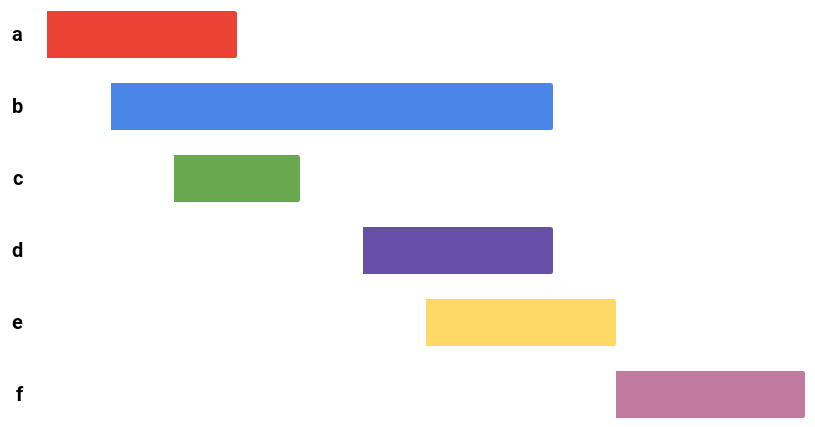
\includegraphics[width=0.9\textwidth]{images/gantt-chart-example.png}
		\captionof{figure}{A Gantt chart featuring six events.}\label{ex:gantt-chart}
	\end{figure}
\end{center}
A chart like this is a useful visual display tool, though it can become a little unwieldy with large numbers of events, and there have been claims that they should be left behind in the field of project management \citep{maylor2001beyond}. Compare the same temporal data in \Cref{ex:gantt-chart} shown in a single string in \cref{ex:gantt-string}:
\begin{align}\label{ex:gantt-string}
	\EventString{{}|a|a,b|a,b,c|b,c|b|b,d|b,d,e|e|f|{}}
\end{align}
No matter how many events may be of interest, if all beginnings, endings, and durations are known---that is, the \textit{temporal closure} has been calculated---such as they could be displayed in a Gantt chart, then they can be represented in a single string, with reducts and projections available in order to focus an analysis on a subset of events if desired, demonstrating a compact method of representing the timeline. However, in general, natural language texts do not provide enough precise temporal detail to determine all of this data. Discourse is typically somewhat vague and relies heavily upon the use of context to determine and precisely temporally locate events. As a result, it's often not possible to immediately derive the temporal closure just from a text, even an annotated text such as one of the documents of the TimeBank \citep{pustejovsky2006timebank} corpus, which is marked up to show the events, times, and temporal relations found within---see also \cref{ssub:timeml}. With that said, even if a single, unified timeline cannot be constructed due to ambiguity, the information in one of these annotated texts may still be extracted and used to build strings, which can provide a visual picture of the content of the document, which may reveal insights not obvious when looking at the text alone.

A string, like a timeline, can be thought of as a simplistic narrative, depicting a world by the events which take place in it. A language of strings, then, is a set of alternate timelines, of parallel worlds. Each string in a language represents a different possible world, describing alternate sequences of the events which took place, and each of which might be considered equally probably to be \textit{veridical}---the actually true world, the correct sequence of events which occurred in reality---without further data and constraints. This allows strings as a framework to capture the ambiguity that very often arises from interpreting the temporal information that is derived from a natural language text. For example, given the information that some event $a$ meets some other event $b$, and $b$ is during some third event $c$, Allen's transitivities---see \Cref{tab:allen-trans-table}, p. \pageref{tab:allen-trans-table}---dictate that the relation between $a$ and $c$ can be one of overlaps, during, or starts. These first two relations $a$ meets $b$ and $b$ during $c$ may be represented by the strings \Meets{a}{b} and \During{b}{c}, respectively---see \Cref{tab:allen-rels-strings}, p. \pageref{tab:allen-rels-strings}---and in fact, the three possible relations between $a$ and $c$ are found by projection relative to $\{a,c\}$ over the result found from superposing thsee two strings, as in \cref{ex:parallel-worlds} below:
\begin{subequations}\label{ex:parallel-worlds}
	\begin{align}
		\Meets{a}{b} \spvc \During{b}{c} = &\{\EventString{{}|c|a,c|b,c|c|{}}, \EventString{{}|a|a,c|b,c|c|{}}, \EventString{{}|a,c|b,c|c|{}}\}\label{ex:parallel-worlds-a}\\
		\text{Under projection to }\{a,c\} = &\{\EventString{{}|c|a,c|c|{}}, \EventString{{}|a|a,c|c|{}}, \EventString{{}|a,c|c|{}}\}\label{ex:parallel-worlds-b}
	\end{align}
\end{subequations}
In \cref{ex:parallel-worlds-a}, the language result of the superposition contains three strings, or three parallel worlds depicting the relational and ordering information that is known about the events $a$, $b$, and $c$, with \cref{ex:parallel-worlds-b} showing the language under projection, which gives three strings depicting the three possible relations between $a$ and $c$---see \Cref{tab:allen-rels-strings}. Unless some further data becomes available constraining these possibilities, there is no way to tell which of the three results of \cref{ex:parallel-worlds-a} is the correct timeline, and so the language as a whole is considered valid. It is important to be wary, though, as too many of these parallel worlds can become unwieldy, just as Gantt charts can become difficult to keep track of if too large a number of events are depicted. One way to avoid an explosion in the number of timelines to keep track of is to avoid superpositions where the inputs do not share some vocabulary, or where the number of strings in the result would exceed some predetermined limit. Another possibility is to alter the granularity of the string, using semi-intervals \citep{Freksa1992} rather than plain intervals, although this does have its own tradeoffs---see \cref{ssub:incomplete}.

Conversely to considering a whole language as valid, occasionally an annotated text may feature inconsistencies, in that relations may be indicated which are impossible for one reason or another, whether that comes from human error on the part of a manual annotator, a poor machine annotation, or simply a text whose narrative is inconsistent. Whatever the source, it is important to be congnisant of these potential issues, as they are likely to lead to at least partially incorrect conclusions being drawn about the timeline of the narrative. Using vocabulary-constrained superposition, these inconsistencies can be discovered as the result of superposing a pair of strings which represent incompatible temporal data will be an empty set. For example:
\begin{align}
	\Before{a}{b} \spvc \During{a}{b} = \emptyset\label{ex:str-inconsistency}
\end{align}
This will always be the case, no matter how many events may appear in either string, and thus the relations between intervals appearing in a string effectively become constraints, which the string models: each string in \cref{ex:str-inconsistency} represents a different constraint, which are incompatible with each other---see also \cref{ssub:zebra}. When doing superposition of languages, if all of the strings from the first language are incompatible with all of the strings from the second, the result will also be an empty language---although, if some of the strings are compatible, then those superpositions are returned, as in \cref{ex:lang-inconsistencies} below, where the only strings which are mutually consistent are the second string of the first language and the first string of the second:
\begin{align}
	\{\EventString{{}|a|{}|b|{}|c|{}}, \EventString{{}|a|b|{}|c|{}}\} \spvc \{\EventString{{}|d|a|b|{}}, \EventString{{}|b,d|a|{}}\} = \{\EventString{{}|d|a|b|{}|c|{}}\}\label{ex:lang-inconsistencies}
\end{align}
A point of interest is that the thirteen interval relations given by the interval algebra of \citet{allen1983maintaining} fall out of the vocabulary-constrained superposition of a pair of strings which each feature a single and different finitely-bounded event\footnote{The superposition of more than two unconstrained intervals in this manner creates a rapidly expanding number of strings. Three intervals gives 409 strings, and by six intervals it has already exceeded three hundred million strings---see \citet[p. 129]{woods2017towards} and the full sequence in \url{https://oeis.org/A055203} \citep{oeisA055203}. This is obviously an excessive amount of information to process, and so generally superposition is to be avoided where there are no constraints between the intervals in one string and the other---that is, where there is no shared vocabulary between the strings to be superposed.}:
\begin{align}
	\mathcal{AR} := \{<,>,m,mi,o,oi,d,di,s,si,f,fi,=\}\label{def:allen-rel-set}\\
	\EventString{{}|v|{}} \spvc \EventString{{}|v'|{}} = \{\mathcal{S}_{\bigcdot}(v,v') ~|~ \bigcdot \in \mathcal{AR}\}
\end{align}
Each string $\mathcal{S}_{\bigcdot}(v,v')$ of the result set features one relation $v \bigcdot v'$, as shown in \Cref{tab:allen-rels-strings}, reproduced from \citet[p. 79, Table 1]{woods2018improving}.
\begin{center}
	\begin{tabular}[h!]{|c|c|c||c|c|c|}
		\hline
		${\bigcdot}$ & $v~{\bigcdot}~v'$ & $\mbox{$\cal{S}$}_{\bigcdot}(v,v')$ & ${\bigcdot}^{-1}$ & $v~{\bigcdot}^{-1}~v'$ & $\mbox{$\cal{S}$}_{{\bigcdot}^{-1}}(v,v')$ \\
		\hline
		$<$ & $v$ before $v'$ & \Before{v}{v'} & $>$ & $v$ after $v'$ & \After{v}{v'} \\
		m & $v$ meets $v'$ & \Meets{v}{v'} & mi & $v$ met by $v'$ & \iMeets{v}{v'} \\
		o & $v$ overlaps $v'$ & \Overlaps{v}{v'} & oi & $v$ overlapped by $v'$ & \iOverlaps{v}{v'} \\
		d & $v$ during $v'$ & \During{v}{v'} & di & $v$ contains $v'$ & \iDuring{v}{v'} \\
		s & $v$ starts $v'$ & \Starts{v}{v'} & si & $v$ started by $v'$ & \iStarts{v}{v'} \\
		f & $v$ finishes $v'$ & \Finishes{v}{v'} & fi & $v$ finished by $v'$ & \iFinishes{v}{v'} \\
		= & $v$ equals $v'$ & \Equals{v}{v'} & & &\\
		\hline
	\end{tabular}
	\captionof{table}{Allen interval relations in strings.}\label{tab:allen-rels-strings}
\end{center}
It can be said that for some string $s$, that $s$ \textit{entails} one of the Allen relations if and only if $s$ projects to the string in \Cref{tab:allen-rels-strings} corresponding to that relation:
\begin{align}
	s \models a \bigcdot b \Longleftrightarrow s \sqsupseteq \mathcal{S}_{\bigcdot}(a, b)\label{def:entails-allen}
\end{align}
Additionally, using the notion of analogous strings (see \cref{para:analogous-strings}, p. \pageref{para:analogous-strings}), any block compressed string which has a vocabulary of cardinality 2 can be compared to the strings in \Cref{tab:allen-rels-strings}. If such a string $s \sim \mathcal{S}_{\bigcdot}(v,v')$ for some $\bigcdot \in \mathcal{AR}$, then the events appearing in $s$ can also be said to be related by $\bigcdot$. For example, $\iFinishes{c}{d} \sim \mathcal{S}_{\text{fi}}(v,v')$, and thus the relation between the events $c$ and $d$ is `$c$ finished by $d$'.

This is easily extended beyond strings featuring just two fluents. The relations between the events appearing in the string $s = \EventString{{}|a|{}|b|{}|c|{}}$ can be determined by taking its block compressed reduct relative to the subsets of the vocabulary which have cardinality 2---in this case, $a$ is before $b$, $b$ is before $c$, and $a$ is before $c$. Once these relations have been calculated, the relations between the events in another string $s' = \EventString{{}|d|{}|e|{}|f|{}}$ are immediately available on analogy $s \sim s'$.

While this is a relatively simple example, it can be extended for strings featuring any arbitrary number of events, and perhaps more usefully it can be used to shortcut superpositions and other string operations. For instance, given the pair of strings $s = \Overlaps{a}{b}$ and $s' = \During{b}{c}$, the vocabulary-constrained superposition is calculated as in \cref{ex:spvc-allen-transitivity}:
\begin{align}\label{ex:sp-analogy}
	s \spvc s' = \{&\EventString{{}|c|a,c|a,b,c|b,c|c|{}}, \EventString{{}|a|a,c|a,b,c|b,c|c|{}},\\
	&\EventString{{}|a,c|a,b,c|b,c|c|{}}\}\notag
\end{align}
Now, given two more strings $t = \Overlaps{x}{y}$ and $t' = \During{y}{z}$ such that $s \sim t$ and $s' \sim t'$, the generated results of superposing $t$ and $t'$ will also be analogous to the results in \cref{ex:sp-analogy}, and so there is no need to calculate $t \spvc t'$. Since the strings are analogous, there is a bijective mapping between the vocabularies $f: (\V_{s} \cup \V_{s'}) \leftrightarrow (\V_{t} \cup \V_{t'})$, and applying this function $f$ to the results in \cref{ex:sp-analogy} gives the same result as calculating the superposition $t \spvc t'$:
\begin{align}\label{ex:sp-analogy-equal}
	f(s \spvc s') = \{&\EventString{{}|z|x,z|x,y,z|y,z|z|{}}, \EventString{{}|x|x,z|x,y,z|y,z|z|{}},\\
	&\EventString{{}|x,z|x,y,z|y,z|z|{}}\}\notag\\
	=~&t \spvc t'
\end{align}
Again, this is a small example, but with larger numbers of events and more complex strings, leveraging the power of analogous strings has the potential to massively reduce the computational cost to calculate superpositions.

By extracting the relations from annotated text as strings and combining them using superposition, a timeline can be built up, which can assist an annotator or other reader in visualising the overall temporal structure of the text. It allows them to check for consistency and also provides a basis for interpreting the narrative in terms of the events that it describes.
% \subsubsection{Inferring New Information}\label{ssub:inferring}
% A text which has been manually annotated for temporal information will typically mark up the most important relations between events, at least as the annotator saw them. By extracting and making plain the timeline, any inconsistencies are immediately revealed, whether these are the fault of a problematic document or human error. Further, relations between times and events which were not previously obvious can be spelled out clearly.

% This can be extended over multiple documents by keeping track of the semantics of the elements in a string---being able to map between the symbols and their meanings---and linking documents which refer to the same events. This can provide a way for checking consistency between reports which originate from different sources, or a way for augmenting an existing timeline with new data.

% Additionally, conclusions can be drawn about whether certain inferences can be made based on existing data by determining the gap between premise strings and strings representing the question statement. That is, deriving the information that could be added to the premises to make the conclusion consistent with the known information (see \cref{ssub:residuals}).

\subsubsection{Constraints and Scheduling (Zebra Puzzle)}\label{ssub:zebra}
Scheduling as a general concept---whereby tasks or events are allocated an ordering according to some set of rules or constraints---is a multi-faceted problem that has been a subject of research for many years \citep{manne1960job,applegate1991computational,pinedo1992scheduling,gong2018memetic}. Available resources must be taken into account, and often it is desirable to find the most efficient way to order the events which are to appear in the schedule so as to minimise the amount of time required for all relevant events to finish. Here it will be shown how the strings described in \cref{sub:strings} can be applied to some scheduling and scheduling-like tasks.

The Zebra Puzzle, also sometimes known as Einstein's Riddle is a logic problem, involving solving a set of clues in order to assign a number of properties to a set of individuals. In the original puzzle, there are five houses in a street, each of a different colour, and in each lives a person of different nationality, who drinks a different beverage, smokes a different brand of cigarettes, and owns a different pet. The puzzle provides clues as to which house contains which set of all of the properties, except that the person who owns a zebra as a pet is not specified, and must be deduced by arranging all of the other elements into their correct houses so that the zebra's home can be determined by process of elimination. This may seem to be a very distinct problem from scheduling, but in fact, there are a number of parallels. Both problems can be viewed as constraint satisfaction problems, and although the Zebra Puzzle concerns spatial constraints, it is not a large stretch to model the street as a sequence of houses, and thus be able to use strings to represent the clues which can be superposed to solve the riddle. If a `house' is conceptualised as a set which contains as elements all of the properties associated with that house---for example, $\{red, english, zebra, coffee, kools\}$---and the street is a sequence of these sets, then the street can be depicted as a string. The left and right spatial relations are thought of in the same way as the previous and subsequent boxes in a string.

To make this connection clearer, below is presented a variant of the puzzle using clues pertaining to temporal relations instead of spatial ones. The clues to the puzzle are as follows in \Cref{tab:temporal-zebra-clues}:
\begin{center}
	\begin{tabular}[h!]{|l|}
		\hline
		There are five weekdays.\\
		The foggy day is mild.\\
		I am tired on the warm day.\\
		There is a traffic jam on the overcast day.\\
		It is cold on the day with little traffic.\\
		It is overcast the day after it snows.\\
		I'm sad the day that I'm reading.\\
		It rains the day I have printing to do.\\
		The traffic is average in the middle of the week.\\
		It's freezing at the beginning of the week.\\
		The stapling is done the day before or the day after I'm happy.\\
		Printing happens the day before or the day after I'm angry.\\
		There is a lot of traffic the day that filing happens.\\
		Shredding happens the day it's hot.\\
		It's freezing the day before or the day after the weather is clear.\\
		\hline
	\end{tabular}
	\captionof{table}{Temporal Zebra puzzle clues in English.}\label{tab:temporal-zebra-clues}
\end{center}
Using these clues, it should be possible to answer these questions:
\begin{itemize}
	\item What day is there no traffic?
	\item What day am I curious? 
\end{itemize}
The puzzle makes three assumptions: first, that the values as presented are \textit{discrete} rather than continuous---`freezing' and `cold', for example, are similar concepts (indeed, if the weather is freezing, then it is also cold), but for the purposes of this puzzle they are treated as being separate and unrelated; second, that each value lasts for only one day---if it rains on one of the days, it will not rain on any other; and third, each day only has one value per attribute---for example, only one task can be performed on any given day. Effectively, recalling that since the strings model inertial worlds, each day contains event-like statives which are treated as having a duration of the entire day. The particular values that appear may make it seem a little absurd---it is rather unlikely that a person would be doing something like printing for a full day, and then immediately begin stapling for another full day, and so on---however, they should suffice for the sake of the example.

For each of the given clues, a constraint can be constructed from one or more strings. Additional constraints can be formed to represent the external assumptions, and by superposing these constraints together, a solution to the puzzle can be found. The strings corresponding to each clue are given in \Cref{tab:zebra-clue-strings}.

For most of the clues, the constraint is formed as a set of a few strings: when event $a$ and $b$ occur on the same day, they will appear in the same box, but it's unknown whether they occur at the beginning of the week (\EventString{a,b|{}}), the end of the week (\EventString{{}|a,b}), or somewhere in the middle (\EventString{{}|a,b|{}}), and so all of the possibilities appear together. It's also worth noting that strings use the Allen relation `meets' where the clue states ``the day before'', rather than the `before' relation. This is due to the fact that one day meets the next, and there is no time between them. The clues which give an event specific position might also have been equivalently written by specifying that the particular value appeared in the same box as one of the day names---for instance \EventString{mon,freezing}. However, the five day names which appear in the first clue of \Cref{tab:zebra-clue-strings} are not actually required for the puzzle: a string of five empty boxes suffices. The names are included here purely for convenience of reading.
\begin{center}
	\onehalfspacing
	\begin{tabular}[h!]{|p{0.9\textwidth}|}
		\hline
		\begin{itemize}
			\item $\{\EventString{mon|tue|wed|thu|fri}\}$
			\item $\{ \EventString{{}|fog,mild},\EventString{{}|fog,mild|{}},\EventString{fog,mild|{}} \}$
			\item $\{ \EventString{{}|tired,warm},\EventString{{}|tired,warm|{}},\EventString{tired,warm|{}} \}$
			\item $\{ \EventString{{}|jammed,overcast},\EventString{{}|jammed,overcast|{}},\EventString{jammed,overcast|{}} \}$
			\item $\{ \EventString{{}|cold,little},\EventString{{}|cold,little|{}},\EventString{cold,little|{}} \}$
			\item $\{ \EventString{{}|snow|overcast},\EventString{{}|snow|overcast|{}},\EventString{snow|overcast|{}} \}$
			\item $\{ \EventString{{}|sad,reading},\EventString{{}|sad,reading|{}},\EventString{sad,reading|{}} \}$
			\item $\{ \EventString{{}|rain,printing},\EventString{{}|rain,printing|{}},\EventString{rain,printing|{}} \}$
			\item $\{\EventString{{}|{}|average|{}|{}}\}$
			\item $\{\EventString{freezing|{}|{}|{}|{}}\}$
			\item $\{ \EventString{{}|stapling|happy},\EventString{{}|stapling|happy|{}},\EventString{stapling|happy|{}},$
			\item[] $~~\EventString{{}|happy|stapling},\EventString{{}|happy|stapling|{}},\EventString{happy|stapling|{}} \}$
			\item $\{ \EventString{{}|printing|angry},\EventString{{}|printing|angry|{}},\EventString{printing|angry|{}},$
			\item[] $~~\EventString{{}|angry|printing},\EventString{{}|angry|printing|{}},\EventString{angry|printing|{}} \}$
			\item $\{ \EventString{{}|lots,filing},\EventString{{}|lots,filing|{}},\EventString{lots,filing|{}} \}$
			\item $\{ \EventString{{}|shredding,hot},\EventString{{}|shredding,hot|{}},\EventString{shredding,hot|{}} \}$
			\item $\{ \EventString{{}|freezing|clear},\EventString{{}|freezing|clear|{}},\EventString{freezing|clear|{}},$
			\item[] $~~\EventString{{}|clear|freezing},\EventString{{}|clear|freezing|{}},\EventString{clear|freezing|{}} \}$	
		\end{itemize}\\
		\hline
	\end{tabular}\captionof{table}{Temporal Zebra puzzle clues as strings.}\label{tab:zebra-clue-strings}
\end{center}
Formally, there are five Attributes (Weather, Temperature, Traffic, Tasks, Mood), each of which is a set of Values. The vocabulary $\V$ of the puzzle is the union of the Attributes:
\begin{itemize}
	\item Weather = $\{rain,clear,fog,snow,overcast\}$
	\item Temperature = $\{freezing,cold,mild,warm,hot\}$
	\item Traffic = $\{none,little,average,lots,jammed\}$
	\item Tasks = $\{printing,stapling,reading,filing,shredding\}$
	\item Mood = $\{happy,angry,sad,tired,curious\}$
\end{itemize}
The external constraints are formalised as follows:
\begin{itemize}
	\item[] ``Each Value only lasts for one day.''
	\item[\ipp\label{impl:zebra-constraintsA}] $\forall v \in \V~ (x \in \llbracket P_v \rrbracket \Longrightarrow \forall v' \in \V~ (v' \neq v \wedge x \notin \llbracket P_{v'} \rrbracket))$
	\item[] ``Each day only contains one Value for each Attribute.''
	\item[\ipp\label{impl:zebra-constraintsB}] $\forall A \in Attributes~ (x \in \llbracket P_v \rrbracket \wedge v \in A \Longrightarrow \forall v' \in A~ (v' \neq v \wedge x \notin \llbracket P_{v'} \rrbracket))$
\end{itemize}
One further constraint is needed due to the nature of superposition allowing for the result of superposing two strings to be longer than either of the input strings:
\begin{itemize}
	\item[]``There are only 5 days.''
	\item[\ipp\label{impl:zebra-constraintsC}] $\forall v \in \V~ (x \in \llbracket P_v \rrbracket \Longrightarrow 1 \leq x \leq 5)$
\end{itemize}
Now, superposing all of the languages in \Cref{tab:zebra-clue-strings} and taking into account the constraints in \cref{impl:zebra-constraintsA,impl:zebra-constraintsB,impl:zebra-constraintsC}, the (singular) result string is generated (each Value is displayed here abbreviated to its first two letters):
\begin{align}
	\EventString{ra,fr,pr,ha|cl,co,li,st,an|fo,mi,av,re,sa|sn,wa,lo,fi,ti|ov,ho,ja,sh}
\end{align}
Finally, superposing this string with languages representing the questions that were asked, a string containing the full ``week schedule" is obtained (\cref{ex:zebra-string-full-solution}), and by taking the reduct of this string relative to $\{none,curious\}$ the solution to the puzzle can be found (\cref{ex:zebra-string-solution-reduct}, and superposed with a string of weekday names for ease of reading in \cref{ex:zebra-string-solution-weekdays}):
\begin{itemize}
	\item $\{\EventString{{}|none}, \EventString{{}|none|{}}, \EventString{none|{}}\}$
	\item $\{\EventString{{}|curious}, \EventString{{}|curious|{}}, \EventString{curious|{}}\}$
\end{itemize}
\begin{subequations}
	\begin{gather}
		\footnotesize
		s = \EventString{ra,fr,pr,ha,\underline{no}|cl,co,li,st,an|fo,mi,av,re,sa|sn,wa,lo,fi,ti|ov,ho,ja,sh,\underline{cu}}\label{ex:zebra-string-full-solution}\\
		\footnotesize
		\rho_{\{none,curious\}}(s) = \EventString{\underline{none}|{}|{}|{}|\underline{curious}}\label{ex:zebra-string-solution-reduct}\\
		\footnotesize
		\rho_{\{none,curious\}}(s) \sp \EventString{mon|tue|wed|thu|fri} = \EventString{mon,\underline{none}|tue|wed|thu|fri,\underline{curious}}\label{ex:zebra-string-solution-weekdays}
	\end{gather}
\end{subequations}
Thus the answer is that ``there is no traffic on the first day of the week", and ``I am curious on the last day of the week". This result is reproduced in \Cref{tab:zebra-solution} below for the sake of completeness.
\begin{ctable}[\label{tab:zebra-solution}]{|r || c | c | c | c | c |}{Solution to Temporal Zebra puzzle as in \cref{ex:zebra-string-full-solution}.}
	\hline
	 & Mon & Tue & Wed & Thu & Fri\\\hline
	Weather & $rain$ & $clear$ & $fog$ & $snow$ & $overcast$\\
	Temperature & $freezing$ & $cold$ & $mild$ & $warm$ & $hot$\\
	Traffic & $\underline{none}$ & $little$ & $average$ & $lots$ & $jammed$\\
	Task & $printing$ & $stapling$ & $reading$ & $filing$ & $shredding$\\
	Mood & $happy$ & $angry$ & $sad$ & $tired$ & $\underline{curious}$\\
	\hline
\end{ctable}
While the Attributes and Values for this variation of the puzzle are relatively meaningless, the use of strings to represent the constraints given in the clues maps well to using strings to model constraints for scheduling problems such as the job-shop problem \citep{manne1960job,applegate1991computational}, wherein a finite number of resources (agents) are available to complete a set of tasks, and an agent can only complete a single task at a time, and the goal is to create a schedule that minimises the maximum of their completion times given that each task also has a specified order that it must be completed in---for instance, task $A$ may only begin after task $B$ is completed, and must be completed before task $C$. This is very similar to the constraints described in the variant of the Zebra Puzzle above, with the additional factor of seeking a string which encapsulates all of the constraints and also has the shortest duration. Another similar problem is the trains example in \citet{durand2008tool}, reproduced below in \Cref{tab:train-problem-clues}, which features six trains arriving and leaving a busy station. The task is to determine the minimum number of platforms needed, given that a train is not allowed to arrive at the same platform while another train is still there.
\begin{center}
	\begin{tabular}[h!]{|l|}
		\hline
		There are 6 trains: $\{A,B,C,D,E,F\}$.\\
		A train may not arrive on a platform if another train has not left that platform.\\
		$\bullet$ $A$, $B$, and $E$ reach the station at the same time.\\
		$\bullet$ $A$ leaves before $B$.\\
		$\bullet$ $A$ leaves after or at the same time as $C$, but before the arrival of $D$.\\
		$\bullet$ $D$ and $F$ arrive at the same time as $B$ is leaving.\\
		$\bullet$ $E$ and $D$ leave at the same time.\\
		\hline
	\end{tabular}
	\captionof{table}{Constraints of the Trains example from \citet[p. 3283]{durand2008tool}.}\label{tab:train-problem-clues}
\end{center}
\citet[p. 3298]{durand2008tool} use a formalism they call S-languages developed based on the concept of S-arrangements \citep{schwer2002s}, which uses arrangements of subsets of elements with repetitions in a manner which is similar in some ways to the string framework described in \cref{sub:strings}, using sequences of elements to represent event-like entities, generally described as either instantaneous points, or in terms of their beginning and end points.

The constraints in \Cref{tab:train-problem-clues} can be represented through the languages in \Cref{tab:train-problem-strings} below, where each `fluent' symbol appearing in a string component represents that train being currently at the station. Therefore, if multiple symbols appear in a box, then each of those trains requires a separate platform at the same time.
\begin{center}
	\singlespacing
	\begin{tabular}[h!]{|p{0.95\textwidth}|}
		\hline
		\begin{itemize}
			\item $\{\EventString{{}|A,B,E|A,B|{}}, \EventString{{}|A,B,E|E|{}}, \EventString{{}|A,B,E|A,B|B|{}},$
			\item[] $~~\EventString{{}|A,B,E|A,E|A|{}}, \EventString{{}|A,B,E|A,E|E|{}}, \EventString{{}|A,B,E|A,B|A|{}},$
			\item[] $~~\EventString{{}|A,B,E|B|{}}, \EventString{{}|A,B,E|A,E|{}}, \EventString{{}|A,B,E|A|{}},$
			\item[] $~~\EventString{{}|A,B,E|B,E|B|{}}, \EventString{{}|A,B,E|{}}, \EventString{{}|A,B,E|B,E|{}}, \EventString{{}|A,B,E|B,E|E|{}}\}$
			\item $\{\EventString{{}|A|{}|B|{}}, \EventString{{}|A|B|{}}, \EventString{{}|A|A,B|B|{}}, \EventString{{}|A,B|B|{}}, \EventString{{}|B|A,B|B|{}}\}$
			\item $\{\EventString{{}|A,C|A|D|{}}, \EventString{{}|C|{}|A|D|{}}, \EventString{{}|C|A|{}|D|{}}, \EventString{{}|C|A,C|{}|D|{}}, \EventString{{}|C|A|D|{}},$
			\item[] $~~\EventString{{}|C|A,C|A|{}|D|{}}, \EventString{{}|A,C|{}|D|{}}, \EventString{{}|A,C|A|{}|D|{}}, \EventString{{}|A|A,C|A|{}|D|{}},$
			\item[] $~~\EventString{{}|C|{}|A|{}|D|{}}, \EventString{{}|A|A,C|{}|D|{}}, \EventString{{}|A,C|D|{}}, \EventString{{}|A|A,C|A|D|{}},$
			\item[] $~~\EventString{{}|C|A,C|A|D|{}}, \EventString{{}|A|A,C|D|{}}, \EventString{{}|C|A,C|D|{}}\}$
			\item $\{\EventString{{}|B|B,D,F|D,F|D|{}}, \EventString{{}|B|B,D,F|D,F|F|{}}, \EventString{{}|B|B,D,F|D,F|{}}\}$
			\item $\{\EventString{{}|E|D,E|{}}, \EventString{{}|D|E,D|{}}, \EventString{{}|D,E|{}}\}$
		\end{itemize}\\
		\hline
	\end{tabular}\captionof{table}{Train scheduling problem constraints as languages of strings.}\label{tab:train-problem-strings}
\end{center}
Superposing these constraints together produces a language of 48 strings, each of which represents a different possible way of satisfying all the scheduling constraints together. In order to determine the minimum number of resources required---in this problem, the number of platforms in the train station---it is simply a matter of finding the string(s) whose largest component is smaller than the largest component of all other strings. In this case, since $B$ and $E$ arrive together, and $D$ and $F$ arrive before either of them have finished leaving, all 48 strings feature a component \EventString{B,D,E,F}---for instance, \allowbreak{}\EventString{{}|C|A,B,E|B,D,E,F|D,E,F|{}}---and thus the minimum number of platforms is the cardinality of that component: four.

Additionally, despite strings not explicitly denoting the durations of events, it is possible to find the timeline which is the least durative by finding the shortest string(s) which uses the maximum possible number of resources. In the case of the trains example, this is \EventString{{}|A,B,C,E|B,D,E,F|D,E,F|{}}. To justify this, consider two events $a$ and $b$ which have durations $\tau_a$ and $\tau_b$, respectively, such that the $a$ lasts longer than $b$, $\tau_a > \tau_b$. In this scenario, four relations are impossible, namely $a$ equals $b$, $a$ during $b$, $a$ starts $b$, and $a$ finishes $b$---all of these imply that $b$ has the same or shorter duration than $a$. Of the remaining nine, the duration of the string representing the relations are as follows in \Cref{tab:rel-durations}\footnote{Disregarding the durations of the empty bounding boxes, which have effectively infinite duration.}:
\begin{center}
	\begin{tabular}[h!]{|c c c|}
		\hline
		\textbf{$\bigcdot$} & \textbf{$\mathcal{S}_{\bigcdot}$} & \textbf{$\tau_{\mathcal{S}_{\bigcdot}}$}\\
		\hline
		$a$ before $b$ & \Before{a}{b} & $\tau_{\mathcal{S}_{\bigcdot}} > \tau_a + \tau_b$\\
		$a$ after $b$ & \After{a}{b} & $\tau_{\mathcal{S}_{\bigcdot}} > \tau_a + \tau_b$\\
		$a$ meets $b$ & \Meets{a}{b} & $\tau_{\mathcal{S}_{\bigcdot}} = \tau_a + \tau_b$\\
		$a$ met by $b$ & \iMeets{a}{b} & $\tau_{\mathcal{S}_{\bigcdot}} = \tau_a + \tau_b$\\
		$a$ overlaps $b$ & \Overlaps{a}{b} & $\tau_a + \tau_b > \tau_{\mathcal{S}_{\bigcdot}} > \tau_a$\\
		$a$ overlapped by $b$ & \iOverlaps{a}{b} & $\tau_a + \tau_b > \tau_{\mathcal{S}_{\bigcdot}} > \tau_a$\\
		$a$ started by $b$ & \iStarts{a}{b} & $\tau_{\mathcal{S}_{\bigcdot}} = \tau_a$\\
		$a$ finished by $b$ & \iFinishes{a}{b} & $\tau_{\mathcal{S}_{\bigcdot}} = \tau_a$\\
		$a$ contains $b$ & \iDuring{a}{b} & $\tau_{\mathcal{S}_{\bigcdot}} = \tau_a$\\
		\hline
	\end{tabular}
	\captionof{table}{Durations of relations between $a$ and $b$.}\label{tab:rel-durations}
\end{center}
As can be seen, a string cannot have a duration shorter than it's longest lasting event, but it may have a duration longer than the sum of all its events. The strings which maximise for component size (overlaps, overlapped by, started by, finished by, contains) all have a duration shorter than those which do not, of which the two shorter strings (meets, met by) have durations shorter than the two longer (before, after). The shortest strings of the maximising five (started by, finished by) have durations equal to the duration of the longest event, $a$. The relations overlaps, overlapped by, and contains all contain a component of the same maximum size, and are the same length, so in the scenario where multiple strings are found to be equally the shortest maximising for component size, a further step would be required to determine the types of relations found in the string---a string with more contains relations should be chosen as being less durative than one with more overlaps or overlapped by relations. Finally, if instead $a$ and $b$ have equal durations, then only one relation is possible between them---$a$ equals $b$, \EventString{{}|a,b|{}}---which also maximises for component size, and has the shortest string length of all the Allen relations.

This chapter has described a framework which uses strings as sequences of sets of temporal entities---times and events---as part of an approach to temporal semantics known as finite-state temporality. Strings of this type are interpretable as finite models of Monadic Second-Order logic, and so due to an equivalence with regular languages, this allows for strings to be recognised by finite-state automata and systems which use them. Several operations are described which can be used to put these strings to work---in particular, the superposition operation allows for strings and sets of strings to be combined, such that all of the temporal data contained therein is incorporated into new strings, and the projection operation allows for determining the linear ordering and relation between a specified subset of times and events in a string.

These operations feed into applications such as deriving timelines from annotated narratives, such as are found in the documents of the TimeBank corpus, a dataset of newswire texts marked up with TimeML, which can be used to provide insight into the overall temporal structure of the text, as well as check for inconsistencies. Additionally, strings can be used as a tool for some kinds of temporal constraint satisfaction, such as in scheduling problems, as the superposition operation can be used to combine strings which model temporal constraints, producing sets of one or more strings in which all the constraints hold successfully, or an empty set if the constraints cannot hold simultaneously.

The next chapter will describe the procedures by which the use of these strings can be integrated with systems which produce semantic annotation for temporal data---primarily focusing on TimeML---and additionally how other resources can be used to augment the work that strings can do, such as being able to make inferences about what relations must be added to a knowledge base in order to be able to draw new conclusions.

\newpage
\section{Methods}\label{sec:methods}
This chapter details the use of strings in application. Using TimeML-annotated documents as a source, strings can be derived from the temporal links, and used to bring out other, implicit relations. However, due to the nature of discourse, the temporal data is often vague or incomplete, so some methods are presented for dealing with this.

\subsection{Extracting Strings from Annotated Text}\label{sub:extracting}
In order to extract temporal strings like those described in \cref{sub:strings} from a text, the text must first be marked up using the TimeML \citep{timeml2005timeml} annotation schema, as this will provide the starting point which indicates which temporal entities are relevant in the text\footnote{Although, if used in an interactive environment such as the tool presented in \cref{sec:implementation}, it is possible to start instead from plain text.}. These annotated times and events, along with the given relations between them, will directly lead to the creation of the initial set of strings, which will serve as a `seed' for the generation of all other possible strings.

Despite TimeML's successor schema, ISO-TimeML \citep{pustejovsky2010iso}, being adopted by the International Organization for Standardization as the standard \citep{ISO24617-1} for semantically annotating temporal data in a text, this work will only focus on the older TimeML version 1.2.1 schema \citep{timeml2005timeml,sauri2006timeml}. The primary source of data is the TimeBank corpus \citep{pustejovsky2006timebank} which is one of the largest available collections of documents which are annotated with any version of TimeML. At the time of writing, the latest release of the corpus is version 1.2, which uses the TimeML version 1.2.1 schema. This corpus is generally seen as a gold standard for any experiments relating to TimeML due to both its size and quality, as it contains 183 documents which were each manually annotated in multiple phases: initially, a pre-processing step wherein five annotators worked on the corpus, regularly meeting to discuss their decisions and improve inter-annotator agreement; the last phase described involved four annotators who ``intimately familiar with the latest specification'' \citep{timeml2005timeml}, which at the time was version 1.2.1, as already mentioned. The documents are amalgamated from a variety of newswire sources, and contain just over 61,000 non-punctuation tokens. The inter-annotator agreement scores (as the average of precision and recall) for the various tag types are given---for a subset of the corpus---below in \Cref{fig:inter-annotator-timebank}, reproduced from \citet{timeml2005timeml}, and it is noted that the low score for the \verb|<TLINK>| tag is due to the large number of event and/or time pairs that may be related to each other, which averages approximately $\frac{(7940+1414)}{183}^2 \approx 2613$ pairs per document.
\begin{center}
	\begin{tabular}[]{|l c c|}
		\hline
		\textbf{Tag} & \textbf{Exact agreement} & \textbf{Partial agreement}\\
		\hline
		TIMEX3 & 0.83 & 0.96\\
		SIGNAL & 0.77 & 0.77\\
		EVENT & 0.78 & 0.81\\
		ALINK & 0.81 & -\\
		SLINK & 0.85 & -\\
		TLINK & 0.55 & -\\
		\hline
	\end{tabular}
	\captionof{figure}{Inter-annotator agreement for tags in TimeBank 1.2\\\citep[from][]{timeml2005timeml}.}\label{fig:inter-annotator-timebank}
\end{center}
The agreement scores are also given for some of the tag attributes, using again the average of precision and recall, and also the kappa scores, reproduced in \Cref{fig:inter-annotator-timebank-attrs}. \citet{timeml2005timeml} does note, though, that due to the size of the subset of documents for which inter-annotator agreement was tested, some of these values are not hugely significant, in particular ``the inter-annotator
agreement numbers for ALINKs as well as the polarity feature for events are not reliable.''
\begin{center}
	\begin{tabular}[]{|l c c|}
		\hline
		\textbf{Tag and attribute} & \textbf{$\frac{precision+recall}{2}$} & \textbf{Kappa}\\
		\hline
		TIMEX3.type & 1.00 & 1.00\\
		TIMEX3.value & 0.90 & 0.89\\
		TIMEX3.temporalFunction & 0.95 & 0.87\\
		TIMEX3.mod & 0.95 & 0.73\\
		EVENT.class & 0.77 & 0.67\\
		MAKEINSTANCE.pos & 0.99 & 0.96\\
		MAKEINSTANCE.tense & 0.96 & 0.93\\
		MAKEINSTANCE.aspect & 1.00 & 1.00\\
		MAKEINSTANCE.polarity & 1.00 & 1.00\\
		MAKEINSTANCE.modality & 1.00 & 1.00\\
		ALINK.relType & 0.80 & 0.63\\
		SLINK.relType & 0.98 & 0.96\\
		TLINK.relType & 0.77 & 0.71\\
		\hline
	\end{tabular}
	\captionof{figure}{Inter-annotator agreement for attributes in TimeBank 1.2\\\citep[from][]{timeml2005timeml}.}\label{fig:inter-annotator-timebank-attrs}
\end{center}
Of most significance to the present work is the favourable score for the \verb|<TLINK>| tags, from which strings can be derived.

\subsubsection{Linking the TLINKs}\label{ssub:tlinks}
TimeML primarily uses \verb|<TLINK>| tags to annotate relations between marked up events and times. These serve as the basis for initial string creation, as they provide information about not only the two intervals that are being related, but also the relation between them. The set of available relations is specific to TimeML---given along with each relation's count and proportion of the TimeBank 1.2 corups in \Cref{tab:timeml-relation-counts}---but has its roots in the set of Allen Relations---see the translation between the sets in \Cref{fig:tlink-allen-translation}, p. \pageref{fig:tlink-allen-translation}. Since Allen's set of relations are what will be used to create strings, the \verb|<ALINK>| and \verb|<SLINK>| tags are ignored for the time being, as are the \verb|<SIGNAL>| tags. The intervals which are being related will be some pairing of event instance IDs and/or time IDs, which point to \verb|<MAKEINSTANCE>| and \verb|<TIMEX3>| tags, respectively, found elsewhere in the document.
\begin{center}
	\begin{tabular}[h!]{| l c c |}
		\hline
		\textbf{Relation} & \textbf{Count} & \textbf{Proportion}\\
		\hline
		BEFORE & 1408 & 21.94\%\\
		AFTER & 897 & 13.98\%\\
		IBEFORE & 34 & 0.53\%\\
		IAFTER & 39 & 0.61\%\\
		DURING & 302 & 4.71\%\\
		DURING\_INV & 1 & 0.02\%\\
		IS\_INCLUDED & 1357 & 21.14\%\\
		INCLUDES & 582 & 9.07\%\\
		BEGINS & 61 & 0.95\%\\
		BEGUN\_BY & 70 & 1.09\%\\
		ENDS & 76 & 1.18\%\\
		ENDED\_BY & 177 & 2.76\%\\
		SIMULTANEOUS & 671 & 10.45\%\\
		IDENTITY & 743 & 11.58\%\\
		\hline
		Total & 6418 & 100\%\\
		\hline
	\end{tabular}
	\captionof{table}{The counts and proportions of each TimeML relation in the TimeBank 1.2 corpus.}\label{tab:timeml-relation-counts}
\end{center}
The decision is made to fold the \verb|<MAKEINSTANCE>| tags into the \verb|<EVENT>| tags which they reference for three reasons: first, this is one of the changes made in ISO-TimeML \citep{pustejovsky2010iso}, which considers the \verb|<EVENT>| tags as explicitly event instances; second, there are 7,940 \verb|<MAKEINSTANCE>| tags in the corpus, and 7,935 \verb|<EVENT>| tags, meaning there are just 5 instances which point at an event already pointed at by another instance---this is just 0.06\% of the instances, so merging them should not have a significant adverse impact; finally, for simplicity's sake, as it makes it easier to track the text in the \verb|<EVENT>| tag along with all of the attributes from the \verb|<MAKEINSTANCE>| tag, like the part of speech, tense, and aspect. While mapping the instances onto the events, it is also necessary to update the \verb|<TLINK>| tags, so that any \verb|eventInstanceID| and \verb|relatedToEventInstance| attributes are converted to \verb|eventID| and \verb|relatedToEvent| attributes, and also updating their values as appropriate.

After folding the tags for events together, a translation is built, mapping from a \verb|<TLINK>| tag to string. The \verb|relType| attribute is extracted from the tag, and converted to an Allen relation by looking up its corresponding relation in \Cref{fig:tlink-allen-translation}, p. \pageref{fig:tlink-allen-translation}. Then, extracting the IDs for the pair of intervals to be related from the \verb|<TLINK>| tag's \verb|eventID| or \verb|timeID| (as $E1$) and \verb|relatedToEvent| or \verb|relatedToTime| (as $E2$) attributes, a string can be constructed using \Cref{tab:allen-rels-strings}, p. \pageref{tab:allen-rels-strings}, replacing $a$ and $b$ in that table with $E1$ and $E2$.

For a minimal example, assume the sentence in \cref{ex:tlink2str-a} is marked up as in \cref{ex:tlink2str-b}, omitting any attributes not directly relevant to this example.
\begin{subequations}
	\begin{itemize}
	\item[\ipp\label{ex:tlink2str-a}] ``John ate dinner, and then washed the dishes.''
	\item[\ipp\label{ex:tlink2str-b}] \verb|John <EVENT eid="e1">ate</EVENT> dinner,|
	\item[] \verb|  and then <EVENT eid="e2">washed</EVENT> the dishes.|
	\item[] \verb|<TLINK eventID="e1" relatedToEvent="e2" relType="BEFORE" />|
	\item[\ipp\label{ex:tlink2str-c}] \verb|BEFORE| $~\equiv~$ $before \in \mathcal{AR}$, $~E1 = $ \verb|e1|, $~E2 = $ \verb|e2|
	\item[\ipp\label{ex:tlink2str-d}] \EventString{{}|e1|{}|e2|{}}
\end{itemize}
\end{subequations}
The relation and two event IDs are extracted from the \verb|<TLINK>| tag in \cref{ex:tlink2str-c} (where $\mathcal{AR}$ is the set of Allen's interval relations, as in \cref{def:allen-rel-set}, p. \pageref{def:allen-rel-set}), which are then arranged according to \Cref{tab:allen-rels-strings}, p. \pageref{tab:allen-rels-strings} to produce the string in \cref{ex:tlink2str-d}.

After mapping from the \verb|<TLINK>| tags to strings, the next step is to start building towards a timeline for the document, by using the vocabulary-constrained superposition technique described in \cref{ssub:operations}, p. \pageref{def:vc-superposition}. This operation will combine the temporal data in pairs of strings, producing a set of output strings which are constrained by the inputs. If the result of a superposition is the empty set, then the input strings were inconsistent with one another---that is, the relations between the fluents in one of the input strings contradicted a relation between those same fluents in the other input. For example, if through some oversight during the annotation process, three events are related by \verb|<TLINK>| tags as follows:
\begin{subequations}
	\begin{itemize}
		\item[\ipp] \verb|<TLINK eventID="e1" relatedToEvent="e2" relType="BEFORE" />|
		\item[\ipp] \verb|<TLINK eventID="e2" relatedToEvent="e3" relType="BEFORE" />|
		\item[\ipp] \verb|<TLINK eventID="e1" relatedToEvent="e3" relType="IBEFORE" />|
	\end{itemize}
\end{subequations}
which produces the following three strings, respectively:
\begin{subequations}
	\begin{align}
		\Before{e1}{e2}\label{ex:tlink-inconsistency-a}\\
		\Before{e2}{e3}\label{ex:tlink-inconsistency-b}\\
		\Meets{e1}{e3}\label{ex:tlink-inconsistency-c}
	\end{align}
\end{subequations}
Attempting to superpose \cref{ex:tlink-inconsistency-a} and \cref{ex:tlink-inconsistency-b} produces a language containing one string---\EventString{{}|e1|{}|e2|{}|e3|{}}---however, when adding the third input string \cref{ex:tlink-inconsistency-c} to the superposition will result in the empty set. The reason why should be clear from the transitivities of Allen's relations---see \Cref{tab:allen-trans-table}, p. \pageref{tab:allen-trans-table}---as $e1 < e2$ and $e2 < e3$ gives that $e1 < e3$ should be found, which is the result of superposing the first two strings, but this is contradicted by the $e1 m e3$ relation in \cref{ex:tlink-inconsistency-c}. By ejecting inconsistencies like this, it is ensured that whatever representation is portrayed to a user is at the very least consistent.

In general, combining the \verb|<TLINK>| tags by superposing their string-translations allows for connections to be built between events and times that were not already explicitly related by the annotation. If every time and event in the document is or becomes related to every other time and event, then the \textit{temporal closure} has been calculated for the document---see \cref{ssub:allen}. For an annotator manually marking up a text with the TimeML schema to give enough detail for the temporal closure to be calculated unassisted would be incredibly difficult, as for $N$ events and/or times in a document there would need to be $\frac{N^2 - N}{2}$ unique \verb|<TLINK>| tags in order to label the relation between each pair, which increases rapidly: at $N = 10$ there are 45 relations, at $N = 50$ there are 1225 relations---while some documents of the TimeBank corups have many less and several have more, the average document has $\frac{7940+1414}{183} \approx 51$ events and/or times. This quickly becomes unwieldy for a human to annotate, especially given that discourse is often vague in the sense that there may not be a clear or even possible way to determine some relations with any kind of precision. For instance, given the following sentence \cref{ex:vague-discourse}, it is clear that both of the leaving events occur after the crash event, but it is not obvious how to label the relation between the two leaving events\footnote{Although, there have been studies which link the order that events appear in the text of a narrative with their temporal ordering, showing that in this example there would be a tendency to assume the police left ahead of the paramedics since they were mentioned first \citep{ohtsuka1992discourse}.}.
\begin{itemize}
	\item[\ipp\label{ex:vague-discourse}] ``After the crash, the police left and the paramedics left.''
\end{itemize}
As such, it should not generally be expected that the temporal closure will already have been computed for any given document---however, if it computed or is computable, then superposing the strings derived from the document's \verb|<TLINK>| tags will ultimately produce a language containing a single string which models the timeline or temporal structure of the document: its vocabulary will be the set of all the events and times in the document\footnote{At least, all of those which were included in at least one TLINK relation. If a time or event was tagged in the text but was not marked up as being related to any other time or event, then there is no way to constrain its relation, and it is effectively an isolated temporal entity, disconnected from the narrative.}, and it will specify the linear ordering and inter-relations of all of these times and events within the context of the document's narrative.

As exemplified in \cref{ex:vague-discourse}, it should be noted that even with the most diligent of annotators, it is still possible that the temporal closure is not immediately computable, as several combinations of the \verb|<TLINK>| relations produce a disjunction of relations which are subsets of the set of Allen Relations according to the transitivities in \Cref{tab:allen-trans-table}, p. \pageref{tab:allen-trans-table}. In these cases, the superposition of the strings derived from the \verb|<TLINK>| tags will produce a language with a number of strings, each representing one possibility from the disjunction of relations. Recall that superposing a pair of languages with each other produces a new language which contains the results of superposing every string from the first language with every string in the second language---this can quickly lead to an explosion in the number of strings that are generated if the relations between the events do not tightly constrain the disjunctions which arise. Take, for example, a document which has tagged within it its document creation time $t0$ and three events $e1, e2, e3$, but the only relations given by the \verb|<TLINK>| tags is that all three of the events occur before the document creation time, and there are no other constraints given on the relations between the three. In this case, vocabulary-constrained superposition will produce a language with 409 strings in it, and if there were four events instead of three, this would already be producing 23,917 strings\footnote{This number increases dramatically quickly with additional intervals, according to the sequence in \citet{oeisA055203}.}, each of which is possibly the true interpretation of the sequence according to all that is known about the document. Obviously this is unwieldy, and in fact for this example superposing the strings like this is no better than guessing the correct linear ordering of the events at random, since superposition is just giving every single possibility. \citet{derczynski2016representation} notes that there needs to be a careful balance between being exact in terms of presenting possible relations, and not letting this set of possible relations grow too large. Assuming for the moment a non-interactive environment where there is no new information forthcoming that can constrain the relations between the events further, there needs to be a way to treat situations like this where the data that can be derived from an annotated text contains some amount of incompleteness, and the temporal closure cannot be computed from just the given knowledge.

\subsubsection{Handling Incomplete Data}\label{ssub:incomplete}
When dealing with any temporal information, there is often a lack of specificity that means the temporal closure---where all intervals in the knowledge base are (consistently) related by exactly one of the set of Allen Relations---for the given document's set of intervals cannot be calculated. For example, take the sentences in \cref{ex:vague-older}:
\begin{itemize}
	\item[\ipp\label{ex:vague-older}] ``Aideen was singing until dinner was served. Brian called Aideen after she had sung.''
\end{itemize}
Assume that for \cref{ex:vague-older}, we have an annotation available which provides two relations between the three events\footnote{In fact, this would be annotated as having a fourth event, `sung', which has the \texttt{IDENTITY} relation with `singing'. The example has been simplified to omit this, but it does not ultimately impact the superposition calculation given in \cref{ex:vague-older-sp}.}, with $e1 = $ `singing', $e2 = $ `served', and $e3 = $ `called'. The relations are that $e1$ meets $e2$, and $e3$ is after $e1$, which are translated to strings as described in the previous section and superposed in \cref{ex:vague-older-sp}, producing a language with five strings in it:
\begin{align}
	\Meets{e1}{e2} \spvc \After{e3}{e1} = \{\EventString{{}|e1|e2|e2,e3|e2|{}}, \EventString{{}|e1|e2|e2,e3|{}},\label{ex:vague-older-sp}\\
	\EventString{{}|e1|e2|{}|e3|{}}, \EventString{{}|e1|e2|e2,e3|e3|{}}, \EventString{{}|e1|e2|e3|{}}\}\notag
\end{align}
The result of the superposition in \cref{ex:vague-older-sp} contains five strings which are each equally valid interpretations of the sequence of the three events, assuming there is no further data with which to constrain the disjunction of strings. While in all five, due to the nature of vocabulary-constrained superposition preserving projections---see \cref{def:vc-superposition}, p. \pageref{def:vc-superposition}---the relation between $e1$ and $e2$ is always `meets', and the relation between $e3$ and $e1$ is always `after', the relation between $e2$ and $e3$ is a disjunction of options. This is seen more clearly by taking the block compressed reduct of each string $s$ in the result of \cref{ex:vague-older-sp} relative to the set $\{e2, e3\}$, as in \Cref{tab:older-strings} below:
\begin{center}
	\begin{tabular}[h!]{| l l |}
		\hline
		$\bc(\rho_{\{e2,e3\}}(s))$ & \textbf{Relation}\\
		\hline
		\EventString{{}|e2|e3,e2|{}} & $e2$ finished by $e3$\\
		\EventString{{}|e2|e3,e2|e2|{}} &  $e2$ contains $e3$\\
		\EventString{{}|e2|e3|{}} &  $e2$ meets $e3$\\
		\EventString{{}|e2|{}|e3|{}} &  $e2$ before $e3$\\
		\EventString{{}|e2|e2,e3|e3|{}} &  $e2$ overlaps $e3$\\
		\hline
	\end{tabular}
	\captionof{table}{Relations arising from the superposition in \cref{ex:vague-older-sp}.}\label{tab:older-strings}
\end{center}
One thing that can be seen in \Cref{tab:older-strings} is that in each string, the leftmost non-empty component always contains just $e2$, implying that $e2$ has begun before $e3$ has begun, although it is not clear which of the two events ends first. In fact, this is exactly the case, and \citet{Freksa1992} uses these kind of disjunctions that can arise as partial justification for their set of 31 semi-interval relations, which are a superset of the Allen Relations. To use semi-intervals, their must be a change in granularity so as to consider the beginnings and endings of intervals as primitive, rather than intervals themselves. In contrast to, for example, \citet{durand2008reasoning} or \citet{Fernando2018}, the beginnings and endings of intervals are themselves intervals, rather than instantaneous points. Since they are intervals, they can also be decomposed into beginnings and endings, depending on how much `zoom' is desired. The major advantage of using beginnings and endings as primitive is that it allows for underspecification of an interval, so that either the beginning or the ending may be omitted from consideration if necessary. This perfectly captures the scenario in \Cref{tab:older-strings}, where the beginning of $e2$ precedes the beginning of $e3$, but the order of their endings is unclear---this corresponds to the Freksa relation labelled `older', and thus $e2$ is older than $e3$.

According to \citet[p. 202]{Freksa1992} there is a ``cognitive awkwardness'' in that, in the case of incomplete information with Allen intervals, the representation becomes more complex the less one knows (as is the case with the example in \Cref{tab:older-strings}), since that knowledge is represented as a disjunction of what \textit{might be} true. He states that, from a cognitive standpoint, the knowledge would be preferably represented ``more directly and in such a way that less knowledge corresponds to a simpler representation than more knowledge does" \citep[p. 202]{Freksa1992}. To address this, Freksa describes the 13 Allen relations in terms of constraints between semi-intervals, as well as 18 more semi-interval relations for situations when it is not (necessarily) known how an event's beginning and ending relate to those of another event \citep[p. 219]{Freksa1992}.

The set of \citet{Freksa1992}'s relations is given in \Cref{tab:freksa-constraints}, showing the constraints which each is associated with, where $l(a)$ and $r(a)$ are the beginning and ending of some interval $a$, and similarly $l(b)$ and $r(b)$ are the beginning and ending of some interval $b$. Allen's relations, which are a subset of Freksa's are omitted from the table, as is the `unknown' relation, which does not impose any constraints on the relation of the intervals nor their beginnings and endings.

The relations are given again in \Cref{tab:freksa-disjunctions}, this time in terms of disjunctions of \citet{allen1983maintaining}'s relations, again excluding Allen's relations and the `unknown' relation, which is a disjunction of all 13 Allen Relations.

It's worth noting here that \citet{Freksa1992}'s primary motivation in the deisgn of these relations was to appeal to the concept of what they called ``conceptual neighbourhoods'', whereby a pair of interval relations are concpetual neighbours if ``they can be directly transformed into one another by continuously deforming (i.e. shortening, lengthening, moving) the events (in a topological sense)'' \citep[p. 206]{Freksa1992}. Thus all of the disjunctions of Allen's relations contain only relations which are conceptual neighbours in this way---for example, it's a shorter cognitive leap to adjust from one event being `before' another to the events having the `meets' relation, than it is to go from `before' to `after'. A subset of these concpetual neighbourhoods can be found as the disjunctions which appear in the transitivity table of \citet[p. 836]{allen1983maintaining}---see \Cref{tab:allen-trans-table}, p. \pageref{tab:allen-trans-table}.
\begin{center}
	\begin{tabular}[h!]{|l c|}
		\hline
		\textbf{Freksa label} & \textbf{Constraints}\\
		\hline
		older & $l(a) < l(b)$\\
		younger & $l(a) > l(b)$\\
		head to head & $l(a) = l(b)$\\
		tail to tail & $r(a) = r(b)$\\
		survives & $r(a) > r(b)$\\
		survived by & $r(a) < r(b)$\\
		precedes & $r(a) \le l(b)$\\
		succeeds & $l(a) \ge r(b)$\\
		born before death & $l(a) < r(b)$\\
		died after birth & $r(a) > l(b)$\\
		contemporary & $l(a) < r(b),~ r(a) > l(b)$\\
		older survived by & $l(a) < l(b),~ r(a) < r(b)$\\
		younger survives & $l(a) > l(b),~ r(a) > r(b)$\\
		older contemporary & $l(a) < l(b),~ r(a) > l(b)$\\
		younger contemporary & $l(a) > l(b),~ l(a) < r(b)$\\
		survived by contemporary & $r(a) > l(b),~ r(a) < r(b)$\\
		surviving contemporary & $l(a) < r(b),~ r(a) > r(b)$\\
		\hline
	\end{tabular}
	\captionof{table}{\citet{Freksa1992}'s relations described in terms of the constraints they impose on the beginnings and endings of a pair of intervals.}\label{tab:freksa-constraints}
\end{center}
\begin{center}
	\begin{tabular}[]{|l l|}
		\hline
		\textbf{Freksa label} & \textbf{Disjunction of Allen's relations}\\
		\hline
		older & before, meets, finished by, contains, overlaps\\
		younger & after, met by, finishes, during, overlapped by\\
		head to head & starts, started by, equals\\
		tail to tail & finishes, finished by, equals\\
		survives & after, met by, started by, contains, overlapped by\\
		survived by & before, meets, starts, during, overlaps\\
		precedes & before, meets\\
		succeeds & after, met by\\
		contemporary & starts, started by, finishes, finished by, during,\\ & contains, overlaps, overlapped by, equals\\
		born before death & before, meets, starts, started by, finishes, finished by,\\ & during, contains, overlaps, overlapped by, equals\\
		died after birth & starts, started by, finishes, finished by, during,\\ & contains, overlaps, overlapped by, equals, after, met by\\
		older survived by & before, meets, overlaps\\
		younger survives & after, met by, overlapped by\\
		older contemporary & finished by, contains, overlaps\\
		younger contemporary & finishes, during, overlapped by\\
		survived by contemporary & during, starts, overlaps\\
		surviving contemporary & contains, started by, overlapped by\\
		\hline
	\end{tabular}
	\captionof{table}{\citet{Freksa1992}'s relations described in terms of disjunctions of \citet{allen1983maintaining}'s relations.}\label{tab:freksa-disjunctions}
\end{center}
In order to take advantage of these relations in strings, first there must be a translation from intervals to semi-intervals, which is described here. First, two predicates are defined:
\begin{align}
	\alpha_v(x) ~:=~ \exists y ~(x < y ~\land~ y \in \llbracket P_v \rrbracket ~\land~ \forall z ~(z < y \Longrightarrow z \notin \llbracket P_v \rrbracket))\label{def:alpha}\\
	\omega_v(x) ~:=~ \exists y ~(y < x ~\land~ y \in \llbracket P_v \rrbracket ~\land~ \forall z ~(y < z \Longrightarrow z \notin \llbracket P_v \rrbracket))\label{def:omega}
\end{align}
\Cref{def:alpha,def:omega} define (for some fluent $v \in \V$) the appearance of $\alpha(v)$ within a box\footnote{Note that it is convenient to write $\alpha(v)$ for $\alpha_v$ when using the box-notation.} as representing a negation of the fluent $v$ conjoined with a formula stating that $v$ will be true in some subsequent box; similarly, $\omega(v)$ represents a negation of the fluent $v$ conjoined with a formula stating that $v$ was true in some previous box. 

A string $s$ may be translated to one using semi-intervals by placing $\alpha(v)$ in every box preceding one in which a fluent $v$ appears, and $\omega(v)$ in every box succeeding it, for each $v \in \V_s$ \citep{woods2018improving}.

For example, a string $s = \EventString{{}|a|b|{}}$ becomes $semi(s)$ in \cref{ex:semi-translated}, in which each of the fluents originally appearing in the string $s$ have also been removed. It's worth highlighting that this representation is possible since, under the semi-interval interpretation, beginnings and endings of intervals are themselves treated as intervals, which is why $\alpha(b)$ and $\omega(a)$ are able to appear in multiple components of the string:
\begin{align}
	semi(s) = \EventString{\alpha(a),\alpha(b)|\alpha(b)|\omega(a)|\omega(a),\omega(b)}\label{ex:semi-translated}
\end{align}
Allowing non-atomic formulas such as these inside the string components does pose a risk of trivialising the work done by superposition, so care must be taken here \citep{woods2018improving}. It should be noticed that strings which use semi-intervals do not (necessarily) feature empty boxes at each end. This is due to the fact that a beginning or ending is only bounded on one side each---if $\alpha(a)$ is true at some moment, stating that the interval $a$ has not yet begun, then it must also be true at every moment before that, since otherwise would imply $a$ having occurred already; similarly for $\omega(a)$ holding at some moment and every moment after it. $\alpha(a)$ may be thought of as `pre-$a$', and $\omega(a)$ as `post-$a$' \citep{woods2018improving}.

This mechanism allows for partially known information to be represented using strings. For example, the string \EventString{\alpha(a), \alpha(b)|{}} represents the knowledge that the events labelled $a$ and $b$ both begin at the same moment, without stating anything about when they each finish---they may end simultaneously, $a$ may finish before $b$, or $b$ may finish before $a$. Which of these states is true is unknown without further data. Going back to the example in \Cref{tab:older-strings}, translating these five strings to use semi-intervals in \Cref{tab:older-strings-semi} makes the relationship amongst them clearer.
\begin{center}
	\begin{tabular}[h!]{| l l |}
		\hline
		\textbf{String} & \textbf{Relation}\\
		\hline
		\siiFinishes{e2}{e3} & $e2$ finished by $e3$\\
		\siiDuring{e2}{e3} &  $e2$ contains $e3$\\
		\siMeets{e2}{e3} &  $e2$ meets $e3$\\
		\siBefore{e2}{e3} &  $e2$ before $e3$\\
		\siOverlaps{e2}{e3} &  $e2$ overlaps $e3$\\
		\hline
	\end{tabular}
	\captionof{table}{Translating strings corresponding to the Freksa `older' relation from \Cref{tab:older-strings} to use semi-intervals.}\label{tab:older-strings-semi}
\end{center}
Leaning on this example a final time, the strings in \Cref{tab:older-strings-semi} are subjected to block compressed reduct relative to the set $\{\alpha(e2), \alpha(e3)\}$ in \Cref{tab:older-strings-semi-bcr}.
\begin{center}
	\begin{tabular}[h!]{| l l |}
		\hline
		$\bc(\rho_{\{\alpha(e2), \alpha(e3)\}}(s))$ & \textbf{Relation}\\
		\hline
		\EventString{\alpha(e2),\alpha(e3)|\alpha(e3)|{}} & $e2$ finished by $e3$\\
		\EventString{\alpha(e2),\alpha(e3)|\alpha(e3)|{}} &  $e2$ contains $e3$\\
		\EventString{\alpha(e2),\alpha(e3)|\alpha(e3)|{}} &  $e2$ meets $e3$\\
		\EventString{\alpha(e2),\alpha(e3)|\alpha(e3)|{}} &  $e2$ before $e3$\\
		\EventString{\alpha(e2),\alpha(e3)|\alpha(e3)|{}} &  $e2$ overlaps $e3$\\
		\hline
	\end{tabular}
	\captionof{table}{Block compressed reduct on \Cref{tab:older-strings-semi}.}\label{tab:older-strings-semi-bcr}
\end{center}
Each of the five strings in \Cref{tab:older-strings-semi} projects (using a block compressed reduct) to the string \EventString{\alpha(e2),\alpha(e3)|\alpha(e3)|{}}, meaning the relation $e2$ is older than $e3$ can be represented using just this one string, instead of a disjunction of five. This does raise the question, however, of whether the tradeoffs are worth it: a great reduction in the cardinality of the timeline set can be achieved, but at the cost of using a more complex vocabulary and reducing the precision of the known information by underspecification.

Out of the 18 non-Allen\footnote{The 13 Allen relations can be represented as single strings using beginnings and endings without underspecification.} Freksa relations, only 11 can be described using a single string without further complicating the vocabulary which may appear within a component (box) of a string. Since all of these new relations are equivalent to disjunctions of Allen relations, it follows that it may be acceptable to include disjunctions of semi-intervals inside a string component, such as \ebox{\alpha(a) \lor \alpha(b)}, which is interpreted as one might expect: either $\alpha(a)$ appears in the component, or $\alpha(b)$ does, or they both do. This allowance admits a further five Freksa relations to be described as single strings. Some relations may be represented in several ways, including the `unknown' relation, which may trivially be described using a single string since it encompasses a disjunction of all 13 Allen relations, and is formed by a simple disjunction of all possible semi-inteval symbols: \ebox{\alpha(a) \lor \alpha(b) \lor \omega(a) \lor \omega(b) \lor \epsilon}, or even more simply, with a string consisting of just a single empty box: \ebox{}.

\Cref{tab:freksa-projections} below shows the 18 Freksa relations and the string which they will project to for some interval events $a$ and $b$. The disjunctions of Allen Relations each Freksa relations corresponds to are given again for convenience, using mnemonic labels\footnote{Using b, bi, and e for $<$, $>$, and $=$, respectively.}.
\begin{center}
	\footnotesize
	\begin{tabular}[h!]{|l | l | c|}
		\hline
		Freksa & Allen & string\\
		\hline
		unknown & b, bi, m, mi, s, si, f, fi, d, di, o, oi, e & \ebox{}\\
		older & b, m, o, di, fi & \EventString{\alpha(a),\alpha(b)|\alpha(b)|{}}\\
		younger & bi, mi, oi, d, f & \EventString{\alpha(a),\alpha(b)|\alpha(a)|{}}\\
		head to head & s, si, e & \EventString{\alpha(a),\alpha(b)|{}}\\
		tail to tail & f, fi, e & \EventString{{}|\omega(a),\omega(b)}\\
		survived by & b, m, s, d, o & \EventString{{}|\omega(a)|\omega(a),\omega(b)}\\
		survives & bi, mi, si, di, oi & \EventString{{}|\omega(b)|\omega(a),\omega(b)}\\
		born before death & b, m, s, si, f, fi, d, di, o, oi, e & \EventString{\alpha(a)|{}|\omega(b)}\\
		died after birth & bi, mi, s, si, f, fi, d, di, o, oi, e & \EventString{\alpha(b)|{}|\omega(a)}\\
		precedes & b, m & \EventString{\alpha(b) \lor \omega(a)}\\
		succeeds & bi, mi & \EventString{\alpha(a) \lor \omega(b)}\\
		contemporary & s, si, f, fi, d, di, o, oi, e & \EventString{\alpha(a) \lor \alpha(b)|{}|\omega(a) \lor \omega(b)}\\
		older contemporary & o, fi, di & \EventString{\alpha(a),\alpha(b)|\alpha(b)|{}|\omega(a) \lor \omega(b)}\\
		younger contemporary & oi, f, d & \EventString{\alpha(a),\alpha(b)|\alpha(a)|{}|\omega(a) \lor \omega(b)}\\
		surviving contemporary & di, si, oi & \EventString{\alpha(a)|{}|\omega(b)|\omega(a),\omega(b)}\\
		survived by contemporary & d, s, o & \EventString{\alpha(b)|{}|\omega(a)|\omega(a),\omega(b)}\\
		older and survived by & b, m, o & ...\\
		younger and survives & bi, mi, oi & ...\\
		\hline
	\end{tabular}
	\captionof{table}{The Freksa relations and the strings they project to.}\label{tab:freksa-projections}
\end{center}
The last two relations in \Cref{tab:freksa-projections}, shown again in \Cref{tab:freksa-projections-b}, cannot be represented using a single string, and are instead must use conjunctions of pairs of strings. What this means is that for the other relations, it can be determined whether some string of semi-intervals $s$ entails that relation if and only if $s$ projects to the string given in \Cref{tab:freksa-projections} for that relation---see also \cref{def:entails-allen}, p. \pageref{def:entails-allen}---for these last two, $s$ will only entail these relations iff it projects to both of the strings given in the conjunction. This may be a small complication, but it is important to address.
\begin{center}
	\footnotesize
	\begin{tabular}[h!]{|l | l | c|}
		\hline
		Freksa & Allen & strings\\
		\hline
		older and survived by & b, m, o & \EventString{\alpha(a),\alpha(b)|\alpha(b)|{}} $\land$ \EventString{{}|\omega(a)|\omega(a),\omega(b)}\\
		younger and survives & bi, mi, oi & \EventString{\alpha(a),\alpha(b)|\alpha(a)|{}} $\land$ \EventString{{}|\omega(b)|\omega(a),\omega(b)}\\
		\hline
	\end{tabular}
	\captionof{table}{The remaining Freksa relations and the strings they project to.}\label{tab:freksa-projections-b}
\end{center}
Now there is a way of representing (almost) all of the disjunctions that may arise from superpositions of strings representing relations between times and events derived from \verb|<TLINK>| tags as single strings. This presents a useful way to tackle the often large sizes of the languages produced when trying to string together the \verb|<TLINK>|s to form a picture of an annotated document's temporal structure in a timeline-like manner. However, there is a notable tradeoff for using semi-intervals instead of intervals, which is that in the process of reducing the cardinality of the output languages, the vocabulary for the strings have become much more complex, with two symbols for every interval where there was only one previously, and including non-atomic formulas such as the disjunctions within string components also adds further complexity to superposition computation. Additionally, the strings which represent some of the Freksa relations are not in all cases necessarily intuitive---for instance, while \EventString{\alpha(a),\alpha(b)|{}} shows neatly that both intervals $a$ and $b$ begin at the same moment for the `head to head' relation, it's not immediately obvious why \EventString{\alpha(b) \lor \omega(a)} should correspond with `precedes'. The additional complexity that arises for the benefit of reducing the amount of data to process threatens the tenet of \citet[p. 202]{Freksa1992} that the representation should not become more complex the less is known.

As such, it would be useful to consider an alternate approach to treating situations where extracting and combining strings from the \verb|<TLINK>| tags of a TimeML document leads to unwieldy numbers of generated strings due to loose constraints from the relation types on the times and events in the narrative. This new approach may be comortably used alongside the semi-interval way of handling if so desired, as shall be shown.

In this treatment, rather than blindly performing vocabulary-constrained superposition between all of the strings which are extracted from the \verb|<TLINK>| tags, which can lead to an explosion of generated strings due to a lack of constraints, only certain pairs of strings will be superposed. Where vocabulary-constrained superposition will produce a language that may contain vastly many strings, a new operation is defined which may only produce at most some fixed number of strings as output. This new operation will avoid superposition if it doesn't make sense to superpose the given strings: when the input strings are the same, the result can only be the same string again; if the strings are not the same, but they have an identical vocabulary, then the strings must contradict each other in terms of the relations they specify among their vocabulary; if the strings don't share any vocabulary, then they cannot constrain each other further through superposition, so no information would be gained; if the size of the language produced by vocabulary-constrained superposition between the languages would be larger than desired. In these last two cases, the input strings are returned so that their data is not lost, and they can potentially be superposed with other strings instead. If none of these situations holds, then the result is just the vocabulary-constrained superposition of the two strings. 

First, set some limit $k \in \mathbb{N}$ which will be the maximum size of the language allowed to be produced. A good default choice for this limit is 12, on the basis that in the case where two intervals are unconstrained relative to each other, they will lead to at least 13 strings being produced by their superposition, which do not add any useful information to the knowledge base. Then, for two strings $s$ and $s'$ the `sensible' superposition $s \sensp s'$ is defined as follows:
\begin{align}
	s \sensp s' := \begin{cases}
		\{s\} &\text{if}~ s = s'\\
		\emptyset &\text{if}~ s \neq s' \land \V_s = \V_{s'}\\
		\{s, s'\} &\text{if}~ \V_s \cap \V_{s'} = \emptyset ~\text{or}~\#(s \spvc s') > k\\
		s \spvc s' &\text{otherwise}
	\end{cases}\label{def:sensible-superposition}
\end{align}
The examples in \cref{ex:sens-sp} demonstrate each of the cases in \cref{def:sensible-superposition}, assuming the limit is set as 12.
\begin{subequations}\label{ex:sens-sp}
	\begin{align}
		\Before{a}{b} \sensp \Before{a}{b} &= \{ \Before{a}{b} \}\\
		\Before{a}{b} \sensp \iMeets{a}{b} &= \emptyset\\
		\Before{a}{b} \sensp \During{c}{d} &= \{\Before{a}{b}, \During{c}{d}\}\\
		\Before{a}{b} \sensp \Before{a}{c} &= \{\Before{a}{b}, \Before{a}{c}\}\\
		\Meets{a}{b} \sensp \During{b}{c} &= \{\EventString{{}|a,c|b,c|c|{}}, \EventString{{}|a|a,c|b,c|c|{}}, \EventString{{}|c|a,c|b,c|c|{}}\}
	\end{align}
\end{subequations}
In order to utilise this choosier form of superposition, one alteration will be made to the process of extracting strings from the \verb|<TLINK>| tags of the TimeBank documents: now, the result of extraction will be a singleton language containing the string, rather than just the string itself. Since the result of superposition of either strings or languages is a language, this change just makes the process a little smoother.

Next, attempt to superpose all of the languages together by iterating through the list, and attempting to perform the sensible superposition for each pair of languages. If the superposition was successful, remove that pair of languages from the list, and add the result of the superposition and start attempting to superpose the languages in the updated list. If there were no successful superpositions after iterating through all the languages, then return the whole list. Since the operation is recursive, this will result in all of the languages being superposed together correctly. The operation is given in pseudo-code below.

\begin{center}
\begin{figure}[h!]
\begin{verbatim}	
superpose_languages(A, B, limit):
  return superpose_sensible(a, b, limit) for a in A, for b in B

superpose_all_languages(list, limit):
  for i=0, i++, i < len(list):
    for j=i+1, j++, j < len(list)
      sp = superpose_languages(list[i], list[j], limit)
      if sp = {}:
        # inconsistent
      elif sp = {list[i], list[j]}:
        # superposition avoided
      else:
        # add the result of superposition and
        # remove the languages that were used
        newList = sp + (list - {list[i], list[j]})
        return superposition_all_languages(newList)
  return list
\end{verbatim}
\end{figure}
\captionof{figure}{Pseudo-code for superposing a list of languages of strings.}\label{fig:pseudo-code-spsens}
\end{center}
The result of this procedure will be a list of languages which were not superposed together---or if all of the languages were superposed, then the list will contain just one language. Each language will contain at most $k$ strings, where $k$ was the pre-determined limit in \cref{def:sensible-superposition}.

To demonstrate the utility of being choosy with when to combine temporal information, an example document is taken from the TimeBank corpus, with a doc ID of \verb|wsj_1073|. The \verb|<TLINK>|s of this document are given below---noting that they have been altered so that the \verb|<EVENT>| and \verb|<MAKEINSTANCE>| were merged.
\begin{center}
	\begin{figure}[h!]
		\begin{itemize}
			\item[] \verb|<TLINK relType="SIMULTANEOUS" eventID="e9" relatedToEvent="e30" />|
			\item[] \verb|<TLINK relType="BEFORE" eventID="e4" relatedToTime="t0"/>|
			\item[] \verb|<TLINK relType="BEFORE" eventID="e2" relatedToTime="t0"/>|
			\item[] \verb|<TLINK relType="BEFORE" eventID="e9" relatedToTime="t0"/>|
			\item[] \verb|<TLINK relType="DURING" eventID="e30" relatedToTime="t31"/>|
		\end{itemize}
	\end{figure}
	\captionof{figure}{TLINKs from the wsj\_1073 document of TimeBank 1.2.}\label{fig:case-study-tlinks}
\end{center}
The strings derived from these tags are in \cref{ex:case-study-strings}:
\begin{align}
	\{\Equals{e9}{e30}, \Before{e4}{t0}, \Before{e2}{t0}, \Before{e9}{t0}, \During{e30}{t31}\}\label{ex:case-study-strings}
\end{align}
Using the normal procedure, these strings are superposed together, and the result is a language containing 7,449 strings, each of which has a vocabulary of $\{e9,e30,e4,t0,e2,t31\}$. Using the sensible superposition along with the procedure in \Cref{fig:pseudo-code-spsens}, the result is a list of three languages: two of which contain a single string, and the third of which contains five strings:
\begin{align}
	\{\EventString{{}|t31|e30,e9,t31|t31|{}|t0|{}}, \EventString{{}|t31|e30,e9,t31|t31|t0,t31|t31|{}},\label{ex:sp-sens-result}\\
	\EventString{{}|t31|e30,e9,t31|t31|t0|{}}, \EventString{{}|t31|e30,e9,t31|t31|t0,t31|t0|{}},\notag\\
	\EventString{{}|t31|e30,e9,t31|t31|t0,t31|{}}\}, \{\EventString{{}|e4|{}|t0|{}}\}, \{\EventString{{}|e2|{}|t0|{}}\}\notag
\end{align}
These seven strings are a lot easier as a human to interpret than the over 7000 from the normal procedure. When one of the languages contains more than one string, as in this case, it is possible to translate these to use semi-intervals, and try to further reduce the cardinality that way, although this may be a case of user preference. The sensible superposition operation is the default option built into the tool presented in \cref{sec:implementation}, although it is possible to remove the limit if desired.


\subsection{Strings From Other Sources}\label{sub:enhancing}
The automatic parsing of the Discourse Representation Structures (DRSs) of Discourse Representation Theory (DRT) \citep{kamp1981theory} from plain text is a field which has recently seen some new approaches \citep{abzianidze2017parallel,van-noord-etal-2018-exploring}, particularly during a recent shared task due to \citet{abzianidze2019first} which aimed to take sentences of English as input and produce DRSs---in an evaluation-friendly clausal form, rather than the typical human-friendly boxed format---as output. The relative success of this task shows that there is an interest in developing systems which can perform automatic DRS parsing. The state-of-the-art was improved considerably, with the winning system of \citet{liu2019discourse} achieving an F1 score of $84.8\%$, an improvement from the baseline score of $54.3\%$. It is possible to leverage the temporal information that features in a DRS to create strings of times and events such as are described in \cref{sub:strings}. While, in general, the temporal relations found using this approach are less specific than those found in TimeML as most parsing tools for DRSs do not appear to utilise Allen's interval algebra, the advantage of using DRSs is that elements such as event participants can be picked out automatically.

Boxer \citep{Bos2008} is one readily available piece of tooling which claims coverage as wide as 95\% for semantic analysis of newswire texts, the same domain as the TimeBank corpus \citep{pustejovsky2006timebank}. The Boxer software is part of the C\&C toolchain \citep{curran2007linguistically} for parsing a text into one or more DRSs, using a neo-Davidsonian representation for events and leveraging the set of thematic roles provided in VerbNet \citep{schuler2005verbnet}, though it is noted in \citet[p. 277]{Bos2008} that the temporal aspects of the tool are not quite as strong as some of the others, and that ``some measure and time expressions are correctly analysed, others aren't.'' A newer version of the tool is used as part of the Parallel Meaning Bank \citep{abzianidze2017parallel} toolchain, although it has not been made widely available for use in research at the time of writing. Another widely available tool for automatic DRS parsing exists as part of the popular Python-based natural language processing toolkit, NLTK \citep{Bird2009}, although it is to be noted that the DRSs produced by this tool do not give much focus to their treatment of events.

\subsubsection{Parallel Meaning Bank}\label{ssub:pmb}
The Parallel Meaning Bank (PMB) is an online corpus (\url{https://pmb.let.rug.nl}) with a total of over 12,000 DRSs for parallel structures in English, German, Dutch, and Italian. The corpus comprises sentences along with clausal form DRSs for providing fine-grained meaning representations for texts, as well as word senses and thematic roles from WordNet \citep{fellbaum2010wordnet} and VerbNet \citep{schuler2005verbnet} respectively.

Under the assumption that the version of Boxer that is used in the PMB would become available at some point, here are some examples of extracting strings from example entries from the corpus. The idea being that, using a high-quality DRS parser to automatically determine semantic information from an unannotated text, then extracting the temporal information from these DRSs to derive strings from could present an opportunity to create a gateway towards automatic temporal annotation: since it is already possible to translate from strings to the \verb|<TLINK>| tags of TimeML \citep{timeml2005timeml}---utilised in the annotation tool described in \cref{sec:implementation}---generating strings from another source could at the very least allow for creating a basic level of semantically informed automatic annotation of a document's temporal relations.

The goal, therefore, is to create a mapping from a text $T$ to some set of strings $S$ which will be used to represent the linear ordering and inter-relations of the temporal entities in $T$. As intermediate steps, $T$ is parsed for semantic information which is represented as one or more DRSs. A projection from these DRSs is created, such that the resultant, reduced DRSs only contain temporal information, and $S$ is the set of strings derived from these temporalised DRSs. The original DRSs are retained in this process so that there is a link back from the representations which have lost all non-temporal information.

Once a DRS representation is parsed from the text, the next step is to eliminate any non-temporal information from the produced DRSs. It is assumed that all temporal information is accurate. A basic approach for how to choose which information to remove is to select all discourse referents which either do not appear in a Time condition or related conditions, such as Duration, or are not explicit time expressions such as \textit{now}, or \textit{09:00}, and then to remove any conditions which featured a now-removed referent. Any now-empty DRSs are also removed. \cref{ex:drs-example} below takes an example from \citet[p. 8]{abzianidze2019first} and shows the text and the originally given DRS, though using the construction that is found in the Parallel Meaning Bank (v2.2.0, ID 99/2308). The conditions in \ref{ex:drs-example-b} which will be retained after projection to \cref{ex:drs-example-c}, the temporalised DRS, are shown in bold.

After removing all of the non-temporal information, a single DRS is left, which in this example corresponds to an instance of not being afraid occurring occurred in the present. This DRS has no information about \textit{who} isn't afraid, or \textit{what} they aren't afraid of, it just represents the \textit{when}.

\begingroup
\setlength{\abovedisplayskip}{-10pt}%
\setlength{\belowdisplayskip}{0pt}%
\setlength{\abovedisplayshortskip}{-10pt}%
\setlength{\belowdisplayshortskip}{0pt}%

\begin{subequations}
	\label{ex:drs-example}
	\begin{align}
	\text{Tom isn't afraid of anything.}\label{ex:drs-example-a}\\
	\text{\drs{$x_1$ \hfill}{
		{\small\texttt{male.n.02($x_1$)}}\\
		{\small\texttt{~~Name($x_1$,tom)}}\\
		$\neg{}$ \drs{$s_1$~~$x_2$~~$t_1$~ \hfill}{
			{\small\textbf{\texttt{time.n.08($t_1$)}}}\\
			{\small\textbf{\texttt{~~$t_1$ $=$ now}}}\\
			{\small\textbf{\texttt{afraid.a.01($s_1$)}}}\\
			{\small\textbf{\texttt{~~Time($s_1$,$t_1$)}}}\\
			{\small\texttt{~~Stimulus($s_1$,$x_2$)}}\\
			{\small\texttt{~~Experiencer($s_1$,$x_1$)}}\\
			{\small\texttt{entity.n.01($x_2$)}}
		}
	}}\label{ex:drs-example-b}\\
	\text{$\neg{}$ \drs{$s_1$~~$t_1$ \hfill}{
		{\small\texttt{time.n.08($t_1$)}}\\
		{\small\texttt{~~$t_1$ $=$ now}}\\
		{\small\texttt{afraid.a.01($s_1$)}}\\
		{\small\texttt{~~Time($s_1$, $t_1$)}}
	}}\label{ex:drs-example-c}\\
	\EventString{|\neg{} s_1, t_1, now|}\label{ex:drs-example-d}
	\end{align}
\end{subequations}
\endgroup
From this reduced DRS in \cref{ex:drs-example-c}, a string can be formed, as in \cref{ex:drs-example-d}. The discourse referents are ordered based on any temporal relations which are mentioned in the DRS's conditions. In this example, \cref{ex:drs-example-d} contains $t_1 =$ \texttt{now}, which indicates that any temporal entities which occur at timepoint $t_1$ are concurrent with the ``current" moment\footnote{Note that there are other uses of \textit{now}, the distinctions dropped here for simplicity.}. This is the time at which the utterance was created, or the time of speech in \citet{reichenbach1947elements}'s framework---see \cref{ssub:tenseaspect}. Other timepoints may be referenced, such as dates, durations, relative times---for example \textit{yesterday}---clock times, and so on, each of which must be ordered correctly.

In addition to the $=$ equals relation, there might be a $\prec$ precedence, $\subset$ during, or $\bigcirc$ overlaps relation, which would correspond to different orderings of the discourse referents. Other conditions, such as negation, are also accounted for---for example, in \cref{ex:drs-example-d} it is assumed that an explicit time expression should not be negated, and so the event expression is negated instead. Although, typically a fluent appearing in a string is negated by its absence from a box, that is, a fluent which appears in the vocabulary of a string is not occurring unless it explicitly \textit{is} occurring. However, event-like statives are treated in TimeML, and may occur as fluents in a string, so it is not too large a step to allow negated fluents into strings.

One further utility of using the DRSs of the Parallel Meaning Bank is the ability to leverage the resources of VerbNet \citep{schuler2005verbnet}, which supplies the semantic roles that permit the new-Davidsonian event semantics in a DRS, and WordNet \citep{fellbaum2010wordnet}, which is used to specify the particular sense of a verb or other word. The version of Boxer used in the PMB includes this information in its output, which may be utilised in linking events that are not given an explicit temporal relation, as events which share semantic participants are likely to be linked in some way.

% \subsubsection{VerbNet and WordNet}\label{ssub:verbwordnet}
% Two resources which are used in the Parallel Meaning Bank \citep{abzianidze2017parallel} and that can be leveraged are VerbNet \citep{schuler2005verbnet}, which supplies the semantic roles that permit the new-Davidsonian event semantics in a DRS, and WordNet \citep{fellbaum2010wordnet}, which is used to specify the particular sense of a verb or other word. The version of Boxer used in the PMB includes this information in its output.

% This data can be useful when trying to make links between events which have not been given a specific relation. For example, finding the closest hypernym between two verbs, or checking verbs which share participants may help to inform the building of relations.

\subsection{Reasoning with Strings}\label{sub:reasoning}
Strings of events may be used to reason about the temporal information they contain: to infer a linear ordering and new relations that were not explicitly stated in the source as existing between the times and events modelled within the strings. There are a number methods which can be employed depending on the specific results that are desired.

Superposition of strings creates new strings which feature all of the constraints of their `parent' strings, and new relations can be derived by taking the projections of these strings in relation to an intersection of the parent vocabularies. %Using resources such as VerbNet and WordNet (see \cref{ssub:verbwordnet}), the lexical semantics can be leveraged in order to suggest links between events which were not previously explicitly related.
Additionally, residuals are employed to determine what relations may need to hold in order for other inferences to be made.

\subsubsection{Superposition and Projection}\label{ssub:superposition}
Given some set of strings, whether extracted from an annotated document, such as one of those in the TimeBank \citep{pustejovsky2006timebank} corpus, or derived from some other source like the temporal properties of DRSs, the most straightforward kind of reasoning that can be done is to use superposition to determine the relations which are not yet made explicit, moving towards the computation of the temporal closure of a document if it is not already calculated. If a document's times and events have temporal closure, then each time and event has been related to each other time and event with exactly one relational label. Once strings have been superposesd together, projection can be used to find the relation(s) that they specify between any pair of times and/or events.

Strings model sets of constraints between the times and events that they mention, and when two strings are superposed, all of these constraints also hold in the resulting language's strings. This can be shown through an example:
\begin{align}
	\Before{a}{b} \spvc \Before{b}{c} = \{\EventString{{}|a|{}|b|{}|c|{}}\}\label{ex:vc-sp-preserve}
\end{align}
The vocabulary-constrained superposition---see \cref{def:vc-superposition}, p. \pageref{def:vc-superposition}---produces a language of all of the strings which have a vocabulary equal to the union of the vocabularies of its inputs and also contain the same constraints as its inputs. For instance, in \cref{ex:vc-sp-preserve} the first input string \Before{a}{b} entails the relation $a$ occurs before $b$, which is also entailed by the sole member of the result language \EventString{{}|a|{}|b|{}|c|{}}. This is due to the fact that vocabulary-constrained superposition preserves \textit{projections}---see \cref{def:projection}, p. \pageref{def:projection}---which can be proven by taking the projection of \EventString{{}|a|{}|b|{}|c|{}} with respect to the vocabulary of \EventString{{}|a|{}|b|{}} and seeing that it is equal to \EventString{{}|a|{}|b|{}}.
\begin{align}
\bc(\rho_{\{a,b\}}(\EventString{{}|a|{}|b|{}|c|{}}))\\ \notag
\bc(\EventString{{}|a|{}|b|{}|{}|{}})\\ \notag
\Before{a}{b}
\end{align}
The string \EventString{{}|a|{}|b|{}|c|{}} thus \textit{projects} to the string \EventString{{}|a|{}|b|{}}, which says that all of the temporal information represented in \EventString{{}|a|{}|b|{}} is also contained within \EventString{{}|a|{}|b|{}|c|{}}. Similarly, the constraint that event $b$ occurs before event $c$ holds in both $\Before{b}{c}$ and in \EventString{{}|a|{}|b|{}|c|{}}; \EventString{{}|a|{}|b|{}|c|{}} projects to \EventString{{}|b|{}|c|{}}.

Since the resulting strings of a vocabulary-constrained superposition always\footnote{Except, of course, if the parent strings are contradictory and the result of superposition is an empty language.} project back to their `parent' strings. they also model the constraints which are represented by each of these parents, although using a single string rather than two strings. However, \EventString{{}|a|{}|b|{}|c|{}} also projects to the string \Before{a}{c}, which represents the constraint that event $a$ occurs before event $c$ according to \Cref{tab:allen-rels-strings}, p. \pageref{tab:allen-rels-strings}. This constraint was not represented in either of the parent strings that were superposed to create \EventString{{}|a|{}|b|{}|c|{}}, but it is represented in this result string. Thus, a new relation between events has been discovered and made explicit. While this example in \cref{ex:vc-sp-preserve} is relatively simple and could be easily derived from simply using the transitivity table for Allen relations---see \Cref{tab:allen-trans-table}, p. \pageref{tab:allen-trans-table}---this procedure works identically for strings featuring an arbitrary number of events, without having to calculate long chains of transitivities. For instance, taking another slightly trivial example for the sake of illustrating the point, imagine a set of events labelled by $a$ through $z$ such that, for each pair of events which are alphabetically adjacent, the `contains' relation holds, so $a$ contains $b$, $b$ contains $c$, ..., $y$ contains $z$. Through superposition of the strings which represent these relations a rather large string is obtained:
\begin{align}
	\EventString{{}|a|a,b|a,b,c|}\cdots\EventString{|a,b,\ldots,y|a,b,\ldots,y,z|a,b,\ldots,y|}\cdots\EventString{|a,b,c|a,b|a|{}}\label{ex:a-z-string}
\end{align}
While it is not hugely difficult to follow along the transitivity chain of this particular set of 25 relations to determine that the relation between $a$ and $z$ is also `contains', it only takes one step to determine this relation while using strings: namely take the projection of the string in \cref{ex:a-z-string} relative to the vocabulary of interest, which in this case is $\{a,z\}$, which produces the string \EventString{{}|a|a,z|a|{}} which entails the `contains' relation between $a$ and $z$, by \cref{def:entails-allen}, p. \pageref{def:entails-allen}. One could further imagine a scenario with the same set of events where the relational transitivities are more difficult to compute, where the relation is not the same for every single event-pair. In this case, superposition will (possibly) produce more than one string as a result, but for every string produced there is exactly one relation between every time or event which appears in that string---effectively, taking each string into consideration in isolation from all of the others, the temporal closure has been computed. In order to find the relation or relations that hold---assuming it is still the relation between $a$ and $z$ that is of interest in this scenario---the projection is taken of each string relative to the set $\{a,z\}$, as before, and the union of all found relations is taken. This set will either be the relation or disjunction of possible relations that may hold between $a$ and $z$.

For a more concrete example, using the sensible superposition operation on the \allowbreak{}\verb|<TLINK>| tags from a document---see \Cref{fig:case-study-tlinks} and \cref{ex:case-study-strings}, p. \pageref{ex:case-study-strings}---from the TimeBank corpus in \cref{ssub:incomplete} produced the set of languages found in \cref{ex:sp-sens-result}. To find, for example, the relation in that document's narrative between the two marked up times, $t0$ and $t31$, the projection of every string across all of the languages is taken relative to $\{t0, t31\}$, producing a set of five strings which correspond to the relations `during', `after', `met by', `finishes', and `overlapped by'. The disjunction of these five are the possibilities for the relation between $t0$ and $t31$, corresponding to the \citet{Freksa1992} relation `younger'.

\subsubsection{Residuals and Gaps}\label{ssub:residuals}
Given some set of strings which represent times and events and their temporal relations to serve as a knowledge base, an operation can be used to determine what strings must be added to the knowledge base in order to make some other string entailed. The operation is known as \textit{gap} as it effectively finds the language that would bridge the gap between the premises (the knowledge base of strings) and the conclusion (the other string).

For example, with the language $L = \{\EventString{{}|a|c|{}}\}$ as the premises and $L' = \{\EventString{{}|b|c|{}}\}$ as the conclusion, the language $gap(L, L') = \{\EventString{{}|a,b|{}}, \EventString{{}|b|c|{}}, \EventString{{}|b|a,b|{}}, \EventString{{}|a|a,b|{}}\}$. Note that the conclusion itself appears in the result, since adding the conclusion to the knowledge base would indeed make it entailed by the knowledge base. Superposing any string from this resulting language $gap$ with the premises should lead to the resulting updated knowledge base entailing the conclusion.

For some pair of arbitrary languages $L, L'$, the $gap(L,L')$ is formed as follows: first, calculate the superposition between the premises and the conclusion.
\begin{align}
	L \spvc L' := \{ s'' ~|~ s \in L,~ s' \in L',~ s'' \in s \spvc s'\}
\end{align}
Next, find the projections $p(L, L')$ in the superposition that, when superposed with the premises, project to the conclusion.
\begin{align}
	p(L, L') := \{\pi_V(s'') ~|&~ s'' \in L \spvc L',~ V \subseteq \V_{s''},\\
	&(\forall s \in L,~\forall s' \in L')(\forall r \in (\pi_V(s'') \spvc s)~ \pi_{\V_{s'}}(r) = s') \}\notag
\end{align}
Define an operation $min(\hat{L})$ that minimises a language $\hat{L}$, such that for any string in $min(\hat{L})$, no other string in $min(\hat{L})$ will project to it.
\begin{align}
	min(\hat{L}) := \{s ~|~ s \in \hat{L}, ~V \subset \V_r, ~\pi_V(r) \notin \hat{L} \}
\end{align}
Then, $gap(L, L')$ is defined as the minimised set $p(L,L')$
\begin{align}
	gap(L, L') := min(p(L, L'))\label{def:gap}
\end{align}
To substantiate the claim that superposing any string from $gap(L,L')$ with the premises produces the conclusion, and the further claim that any string in the superposition of $L$ with $L'$ projects to some string in $gap(L, L')$, $gap(L, L')$ will be related to the residual $L'/L$ of $L'$ by $L$, relative to superposition as a binary operation on languages of block compressed strings.

First fix some large set of symbols $\Theta$, with $Fin(\Theta)$ as the set of finite set of subsets of $\Theta$. For any $A \in Fin(\Theta)$, define the set of all block compressed strings whose vocabulary is in $A$
\begin{align}
	\mathcal{L}_A := \{ \bc(s) ~|~ s \in (2^A)^* \}
\end{align}
and for any $s \in Fin(\Theta)^*$, let
\begin{align}
	\llbracket s \rrbracket_A := \{s' \in \mathcal{L}_A ~|~ s' \sqsupseteq s\}
\end{align}
which is lifted to languages disjunctively, with the implication that $\llbracket s \rrbracket_A = \llbracket \{s\} \rrbracket_A$
\begin{align}
	\llbracket L \rrbracket_A := \bigcup ~ \{\llbracket s \rrbracket_A ~|~ s \in L \}
\end{align}
Note then that
\begin{align}
	L \sqsupseteq L' \Longleftrightarrow \llbracket L \rrbracket_A \subseteq \llbracket L' \rrbracket_A
\end{align}
where $L \sqsupseteq L'$ says that the language $L$ projects to $L'$---see \cref{def:lang-projection}, p. \pageref{def:lang-projection}---and also
\begin{align}
	\llbracket L \spvc L' \rrbracket_A = \llbracket L \rrbracket_A \cap \llbracket L' \rrbracket_A
\end{align}
The first claim, that superposing any string from $gap(L,L')$ with the premises produces the conclusion, comes to
\begin{align}
	\llbracket L \rrbracket_A \cap \llbracket gap(L, L') \rrbracket_A \subseteq \llbracket L' \rrbracket_A
\end{align}
and the second claim, that any string in the superposition of $L$ with $L'$ projects to some string in $gap(L, L')$
\begin{align}
	\llbracket L \rrbracket_A \cap \llbracket L' \rrbracket_A \subseteq \llbracket gap(L, L') \rrbracket_A
\end{align}
For residuals, let
\begin{align}
	res_A(L, L') := \{s \in \mathcal{L}_A ~|~ \llbracket s \rrbracket_A \cap \llbracket L \rrbracket_A \subseteq \llbracket L' \rrbracket_A \}
\end{align}
noting that, for all $L, L', L'' \subseteq \mathcal{L}_A$
\begin{align}
	\llbracket L \rrbracket_A \cap \llbracket L'' \rrbracket_A \subseteq \llbracket L' \rrbracket_A \Longleftrightarrow \llbracket L'' \rrbracket_A \subseteq res_A(L, L')
\end{align}
To find the connection between $res$ and $gap$, first define the \textit{downset} $L_\downarrow$ of $L$ as the set of all strings which the strings in $L$ project to
\begin{align}
	L_\downarrow := \{ \pi_V(s) ~|~ s \in L,~ V \subseteq \V_s \}
\end{align}
And so
\begin{align}
	p(L, L') = \{s \in (L \spvc L')_\downarrow ~|~ (\{s\} \spvc L) \sqsupseteq L'\}
\end{align}
Observe that, for any $\hat{L}$
\begin{align}
	\llbracket min(\hat{L}) \rrbracket_A = \llbracket \hat{L} \rrbracket_A
\end{align}
and since $gap(L, L')$ is just equal to $min(p(L, L'))$
\begin{align}
	\llbracket gap(L, L') \rrbracket_A = \llbracket res_A(L, L') \cap (L \spvc L')_\downarrow \rrbracket_A
\end{align}
The gap operation is useful for using strings in the context of question-answering systems, for example in the FRACAS semantic test suite \citep{cooper1996using}, and allows for inferences to be made about whether certains relations could possibly exist given some knowledge base of strings.

The next chapter describes the details of how the string framework which was described in \cref{sec:fst} and used throughout the current chapter is currently implemented. In particular, an illustrative tool is discussed which may be used to annotate text with a slightly modified subset of the TimeML 1.2 \citep{timeml2005timeml} schema, or to edit and examine a document that has already been marked up.
\newpage
\section[String Temporal Annotation and Relation Tool (START)]{String Temporal Annotation and Relation Tool\\(START)}\label{sec:implementation}
In order to implement the string framework for representing times and events as described in \Cref{sec:fst} and utilised in \cref{sec:methods}, various approaches were trialled using different programming languages, including Prolog, JavaScript (Node.js), and Python \citep[see][respectively for more on each]{clocksin2012programming,tilkov2010node,kuhlman2009python}. Ultimately, Python (version 3) was chosen for its speed, wide cross-platform availability, and ease of use through familiarity.

Python is a high-level, dynamically-typed, interpreted programming language implemented in C, with a large standard library that has found widespread use among scientific communities, in part thanks to the availability of tooling such as the Natural Language Toolkit (NLTK) \citep{Bird2009} for natural language processing and PyTorch \citep{ketkar2017introduction} for machine learning, as well as many other packages which are easily accessible through an official package installer.

Although Python has support for object-oriented programming styles, a functional programming paradigm was used in the design of the framework, wherein the use of mutable, global state is avoided. Functions are designed so as to take some input and give some output, without causing side effects, so that running a function with a particular input will always give the same result. This style of programming was chosen so as to better reflect the logical forms of the string operations which are described in \cref{ssub:operations}---a mathematical function has no state, it simply takes some input and transforms it into an output.

In order to illustrate what is enabled by the use of the string framework, a proof-of-concept tool for annotation was built as a web-based application (though, with a little effort, it may also be downloaded and set up to be used locally without an internet connection), which is available at \url{http://scss.tcd.ie/~dwoods/thesis/code/start}\footnote{Also available at \url{https://start-dwoodscs.vercel.app}.}, and all of the code is available to view at \url{https://github.com/dave-woods/thesis/tree/master/code/start}. The main drive behind this tool is on using strings for discovery and consistency-checking of relations between a document's times and events, while providing a useful visual aid for a human annotator to verify that the timeline of the document, inasmuch as it can be determined, lines up with their understanding of the narrative's temporal structure.

The front-end of the application, known as START for String Temporal Annotation and Relation Tool, was developed and built using the Next.js (\url{https://nextjs.org}) framework upon top of the React (\url{https://reactjs.org}) JavaScript library, both of which are open source software. React is designed for building fast user interfaces through a component-based library that only updates the parts of the web page's document object model (DOM) which need to be updated, rather than re-rendering the entire page on every request or interaction sent from the page. Next.js enables web pages to be rendered on the server rather than on the client's machine, and provides some extra abstractions over common tasks in React. Next.js is also tightly integrated with the cloud-based hosting platform Vercel (\url{https://vercel.com/docs}) which allows for Python code to be hosted as part of the application in the form of so-called serverless functions \citep{anderson1995serverless} where ``application logic is split into functions and executed in response to events'' \citep[p. 405]{mcgrath2017serverless}. The result of this is that for most operations of the string framework made from the application, the client will send a request to an API endpoint hosted by Vercel. On receiving the request, Vercel will trigger the appropriate function from the string framework with any data passed along with the API request, using JSON as a format for communication between the front-end and back-end. Once the function has completed, it returns any data (or errors) to the client to be used or displayed as appropriate.

For the reader's convenience, two video files are available which demonstrate the tool in use. The first is located at \url{https://www.scss.tcd.ie/~dwoods/thesis/code/assets/annotate-text.mp4} and shows the process of working with a pre-annotated TimeML file. The second is located at \url{https://www.scss.tcd.ie/~dwoods/thesis/code/assets/annotate-plain-text.mp4} and shows the process of working with and adding annotation to plain text.

An important note for understanding the notation in the code and the tool is that, since strings of times and events as used in the current work are sequences of sets of symbols, the appropriate format to represent these in the code would be lists of sets---and indeed, this is the underlying representation. However, since both Python and JavaScript have strings as built-in types, an alternative but equivalent representation is used to write the strings. This increases their portability, since list in Python and arrays in JavaScript are heavier objects that use more memory than the built-in strings. In this new notation, the pipe character `$|$' is used to denotate the boundary between two consecutive string components. For example, the string \EventString{{}|a|a,b|b|{}} can be written as ``\verb!|a|a,b|b|!''. A simple function can translate from a string of this kind to a list of components and back again.

\subsection{Back-end API}\label{sub:backend} % ?NLTK
The majority of the implementation of the framework is contained within a single Python file, which is called \verb|strfns.py| in the Appendices. Following the functional programming style meant that any of the operations defined in \cref{ssub:operations} would be implemented by composing together several Python functions, each of which has a single clear task. The functions need to be pure, meaning that they have no side effects, and running a function any number of times on the same input will produce the same output every time. As such, the \verb|strfns.py| file contains only functions---in order to use them, they must be imported into another file, which is exactly what happens in the other Python files included in the Appendices. In fact, all of the other Python files also only define functions---these are the serverless functions which are hosted by Vercel. When the front-end sends a request to one of these endpoints, the \verb|handler| class in each of \verb|freksa.py|, \verb|newTLINKs.py|, \verb|superpose.py|, and \verb|test.py| triggers the (sole) function it contains, \verb|do_POST|, which performs the requested data manipulations and sends the results back to the client.

There is, however, one caveat to the purity of the \verb|strfns.py| file, which is that the \verb|superpose_sensible| function uses a decorator which implements a LRU-style cache from the standard \verb|functools| library. The decorator wraps the function in another function, encapsulating it and giving it access to a cache object which uses the LRU stategy: that is, the `Least Recently Used' items in the cache will be removed to make room for new items---compare with a FIFO or `First In First Out' strategy which says that newer entries are the most likely to be reused, where LRU says that recently used entries are the most likely to be resused. So technically the \verb|superpose_sensible| function does have a side effect of potential cache mutation, rather than being a completely pure function. However, for all intents and purposes it is still essentially pure, in that passing the function the same inputs will always produce the same outputs, it'll just retrieve them from the cache rather than computing them after the first time.

Since the algorithm for computing the sensible superposition of a list of languages---see \Cref{fig:pseudo-code-spsens}, p. \pageref{fig:pseudo-code-spsens}---involves a nested for-loop as well as recursion, the tradeoff for sacrificing a little functional purity and some memory space is a dramatic increase in efficiency. This can be seen best through example, so going back to the \verb|wsj_1073| file from the TimeBank corpus, the strings derived from the \verb|<TLINK>| tags and the result of sensibly superposing these are reproduced from \cref{ex:case-study-strings} and \cref{ex:sp-sens-result} below for convenience.
\begin{align}
	\{\Equals{e9}{e30}, \Before{e4}{t0}, \Before{e2}{t0}, \Before{e9}{t0}, \During{e30}{t31}\}\label{ex:caching-strs}
\end{align}
\begin{align}
	\{\EventString{{}|t31|e30,e9,t31|t31|{}|t0|{}}, \EventString{{}|t31|e30,e9,t31|t31|t0,t31|t31|{}},\\
	\EventString{{}|t31|e30,e9,t31|t31|t0|{}}, \EventString{{}|t31|e30,e9,t31|t31|t0,t31|t0|{}},\notag\\
	\EventString{{}|t31|e30,e9,t31|t31|t0,t31|{}}\}, \{\EventString{{}|e4|{}|t0|{}}\}, \{\EventString{{}|e2|{}|t0|{}}\}\notag
\end{align}
The LRU cache implementation allows for a maxsize to be set, so the most recently used 1000 (string) superpositions are kept in the cache, which can vastly improve the speed of the calculation. Using Python's built-in \verb|timeit| functionality to test how much time repetitions of a function takes\footnote{Running with Python v3.7.3 (64-bit) on Ubuntu 16.04 using an Intel i7-6700 CPU with 16GB memory.}, with the input from \cref{ex:caching-strs}, we find the following times while varying whether sensible superposition used the cache or not:
\begin{center}
	\footnotesize
	\begin{tabular}[h!]{|r|c  c  c|}
		\hline
		\textbf{Iterations} & \textbf{No caching (s)} & \textbf{Caching (s)} & $\frac{caching}{no caching}$ (\%)\\
		\hline
		1 & 0.02069 & 0.00018 & 0.87\%\\
		100 & 1.61041 & 0.0063 & 0.39\%\\% 32 vs 100
		10000 & 163.17628 & 0.26268 & 0.16\%\\% 98 vs 14
		\hline
	\end{tabular}
	\captionof{table}{Caching superpositions vastly improving efficiency.}
\end{center}
On average, the version using caching took less the half of one percent of the time that the non-caching version took. Since these functions are to be used as part of an API which forms the back-end to a web-based application, long waiting times are very undesirable. An annotator using a tool does not want to have to wait for the tool to keep up with them---really, a tool that makes itself noticeable for any reason rather than just facilitating the task at hand is problematic.

% Just for comparisons sake, using vocabulary-constrained superposition with the same inputs, in comparison with the non-caching sensible superposition.
% \begin{center}
% 	\footnotesize
% 	\begin{tabular}[h!]{|r|c  c  |}
% 		\hline
% 		\textbf{Iterations} & \textbf{$\sensp$ (s)} & \textbf{$\spvc$ (s)}\\
% 		\hline
% 		1 & 0.02069 & 0.43679\\
% 		10 & 0.47613 & 4.0403\\
% 		100 & 1.61041 & 40.9049\\
% 		1000 & 0.02069 & 408.9788\\
% 		\hline
% 	\end{tabular}
% 	\captionof{table}{Caching superpositions vastly improving efficiency.}
% \end{center}
Other than the superposition algorithm, there are also a number of functions defined for reasoning with strings. In particular, there are a set of projection functions which use the definition of projection in \cref{def:projection}, p. \pageref{def:projection} and extend it so that there are definitions of a language projecting to a string if all strings in the language project to the string, a language projecting to a language if all strings in the first language project to all strings in the second, a language containing a string if some string in the language projects to it, and a language contradicting a string if the language doesn't contain it and there is some string in the language whose vocabulary contains the vocabulary of the string.
\begin{align}
	L \sqsupseteq s' &\Longleftrightarrow \forall s \in L ~(s \sqsupseteq s')\\
	L \sqsupseteq L' &\Longleftrightarrow \forall (s \in L,~ s' \in L')~(s \sqsupseteq s')\\
	contains(L, s') &\Longleftrightarrow \exists s \in L ~(s \sqsupseteq s')\\
	contradicts(L, s') &\Longleftrightarrow \lnot contains(L, s') \land \exists s \in L ~(\V_s \supseteq \V_{s'})
\end{align}
These functions are used as part of the relation testing procedure while annotating a text with TimeML---when a user wants to add some relation between a pair of events or times, which will be added in the form of a string, first it is reasonable to test whether that string and relation are possible given the current knowledge base of relations, or if it's even contradicted by some other relation.

There's also an implementation of the gap algorithm described in \cref{ssub:residuals} which calculates the set of strings which would need to be superposed with some premises in order to entail some conclusion, an algorithm to determine which string of some list uses the least simultaneous resources, which helps to answer the trains problem in \Cref{tab:train-problem-clues}, p. \pageref{tab:train-problem-clues}, and functions to translate to and from between a string using intervals and a string using semi-intervals, as described in \cref{ssub:incomplete}.

The file \verb|freksa.py| is effectively a lookup table, providing the set of strings which correspond with any given relation from either Allen's set or the extended Freksa set. \verb|newTLINKs.py| uses the concept of analogous strings---see \cref{para:analogous-strings}, p. \pageref{para:analogous-strings}---to determine the TimeML \verb|<TLINK>| relation type to use when translating back from strings during the export process of the START application.

\subsection{Front-end Interface}\label{sub:frontend}
A web-based application was chosen for the graphical user interface (GUI) as this ensures the widest coverage in terms of accessibility, as the only requirement is a modestly up-to-date web browser. It is possible to download the system and run it locally, but it's not envisioned that there would be much need unless planning to annotate without a web connection for an extended period of time. The key benefit of running the application in a web browser is that there is no need to download or install anything to get started, and additionally being able to design the GUI using HTML and CSS is somewhat more straightforward than some of the existing GUI toolkits for Python---again, there is no need to download or install anything new, as everything operates within the same interface.

On visiting the web page at \url{http://scss.tcd.ie/~dwoods/thesis/code/start}, the user is greeted with a blank textarea input. Most of the functionality is inactive until some text has been entered into this input. There are two sample files from the TimeBank corpus \citep{pustejovsky2006timebank} linked on the lower left of the screen, which the user can copy into the textarea to get a feel for how to use the tool. Once the user clicks the `Annotate' button, the system will try to parse the input as a TimeML file, but if it fails to parse it, then it will be considered as plain text. If this is the case, then all of the features described below will work just the same, but the user will have to begin marking up from scratch, as there must be some tagged events or times to begin with before they can be related and the relation transformed into a string.
\begin{center}
	\begin{figure}[h!]
		\centering
		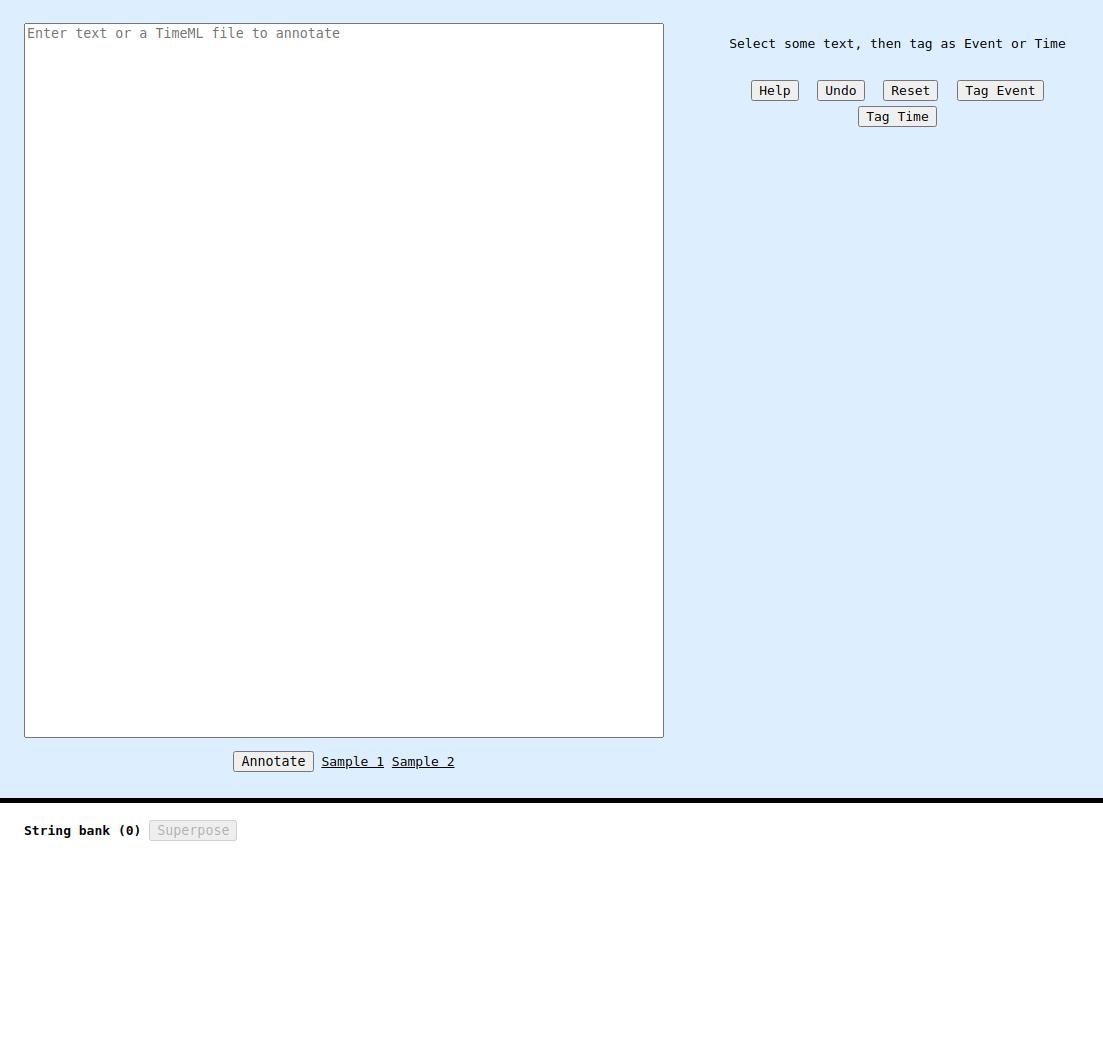
\includegraphics[width=0.9\textwidth]{images/START-blank.png}
		\captionof{figure}{START: Initial blank input.}
	\end{figure}
\end{center}
Assuming the user chose to input some TimeML\footnote{The file used in the below screenshots is the `Sample 1' file available on the web page, which is the same document of the TimeBank corpus used in the example in \Cref{fig:case-study-tlinks}, document ID \texttt{wsj\_1073}.}, the input area will change to instead show the text content of the inputted document with the times and events highlighted in pink and yellow, respectively. All of these times and events are also added to a list on the right-hand side of the screen---noting that \verb|<EVENT>| and \verb|<MAKEINSTANCE>| tags have been amalgamated as described in \cref{ssub:tlinks}. Finally, the strings that are derived from the \verb|<TLINK>| tags are added to the `String bank' section in the lower left of the screen, and a new panel becomes available on the lower right side.
\begin{center}
	\begin{figure}[h!]
		\centering
		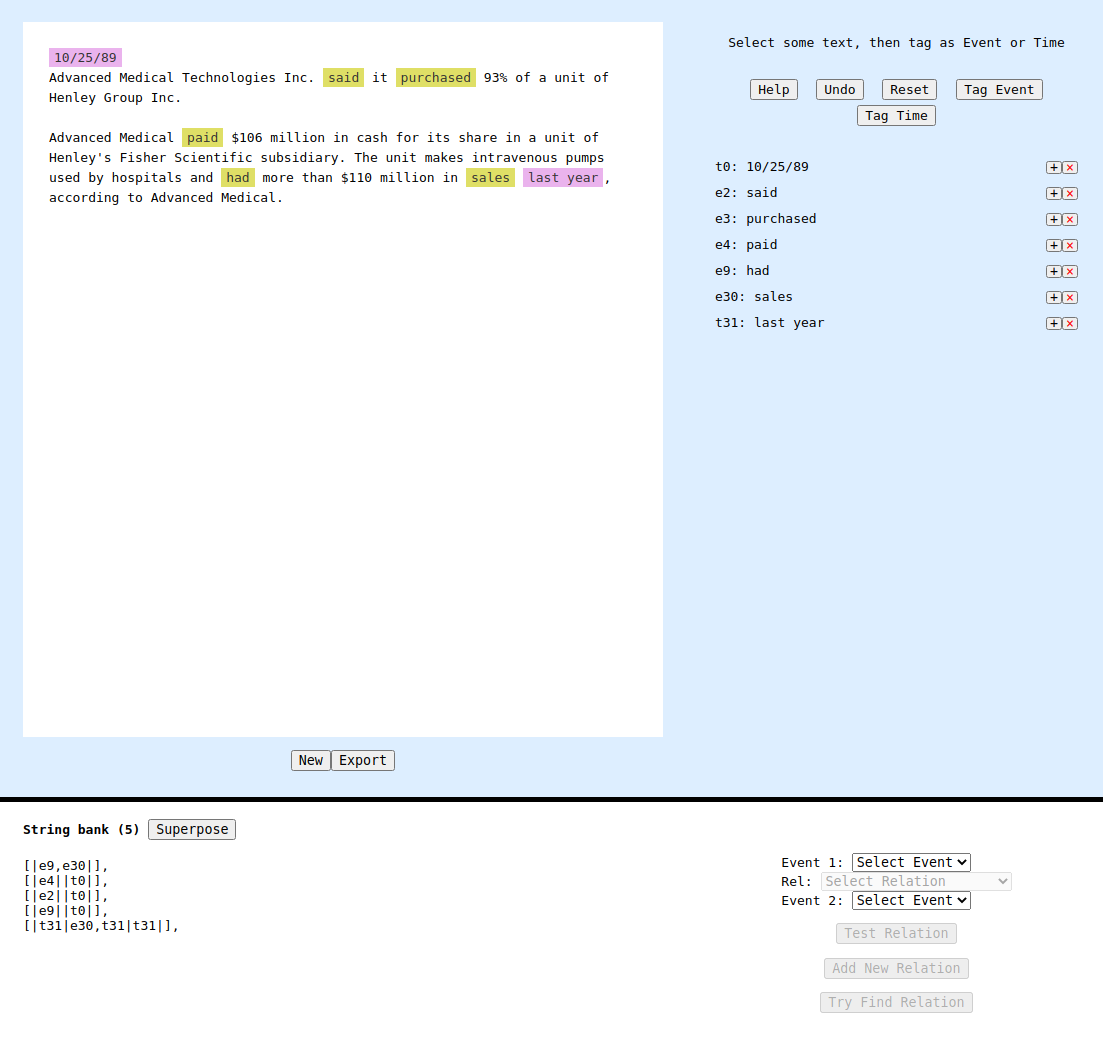
\includegraphics[width=0.9\textwidth]{images/START-imported.png}
		\captionof{figure}{START: The screen after a TimeML file is imported.}
	\end{figure}
\end{center}
At this point the user is in the main flow of the system. They are free to immediately click the `Export' button to export the data to a new TimeML file and leave the program if they wish---noting that the export works from what the system knows of the data, rather than basing it on the original input. Internally, since the relations are stored as strings, which use Allen's set rather than the TimeML set, and some of the TimeML relations map to the same Allen relation---see \Cref{fig:tlink-allen-translation}, p. \pageref{fig:tlink-allen-translation}---it is possible that the relations specified in the original document will be different from those in the exported one, though it is guaranteed that they will map to the same Allen relation. Also, it is worth bearing in mind that the TimeML that is exported is a subset of the full schema, so the \verb|<SIGNAL>|, \verb|<SLINK>|, and \verb|<ALINK>| tags are ignored, as they are not directly involved in the computations relating to temporal ordering.

If the user doesn't in fact leave immediately, they may notice that the temporal relations found in the document have been imported as languages of strings.
\begin{center}
	\begin{figure}[h!]
		\centering
		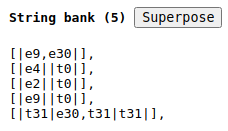
\includegraphics[width=0.4\textwidth]{images/START-sp-1.png}
		\captionof{figure}{START: The String bank after importing TimeML.}
	\end{figure}
\end{center}
Clicking on the `Superpose' button or pressing the S key on the keyboard will send a request to the back-end to compute the sensible superposition of all of the languages in the String bank, which may result in a smaller number of languages, as it does in this case. The strings have been combined where it made sense to do so and the result of superposition did not create a language with a cardinality greater than the set limit---see \cref{def:sensible-superposition}, p. \pageref{def:sensible-superposition}. The limit is initially set to a default value of 12, so that strings which do not constrain each other tightly will not be superposed, though this limit can be altered by clicking the `Help' button. Setting the limit to a value of 0 will perform the superposition without a limit at all, though this can produce unwieldy results and may be slower in terms of performance, so is not recommended if not necessary. If, during superposition, an empty set is ever returned from Python, this implies that an inconsistency was present in some of the strings in the String bank. The system will warn the user that a problem was found, and it will show the languages that were being superposed when the error occurred.
\begin{center}
	\begin{figure}[h!]
		\centering
		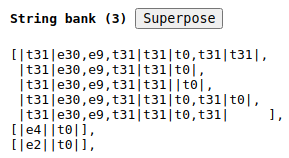
\includegraphics[width=0.4\textwidth]{images/START-sp-2.png}
		\captionof{figure}{START: The String bank after clicking `Superpose'.}
	\end{figure}
\end{center}
If the user hovers their mouse over one of the strings in the String bank, all of the highlights in the main text area will turn off except for any times and events that are mentioned in that string. If the user clicks on a string, an overlay will appear which shows the string in the conventional notation established in \cref{sub:strings}, with the event text appearing in place of the time or event IDs, so as to help the user decide whether the string seems valid or not, for example in the case of trying to narrow down a disjunction. A list of all the \verb|<TLINK>| tags which can be derived from the string is also displayed. If the user wishes to remove the string from the knowledge base for whatever reason, the `Remove' button at the top of the panel will do this. The user can press the Escape key, or click outside the panel to return to the main screen.
\begin{center}
	\begin{figure}[h!]
		\centering
		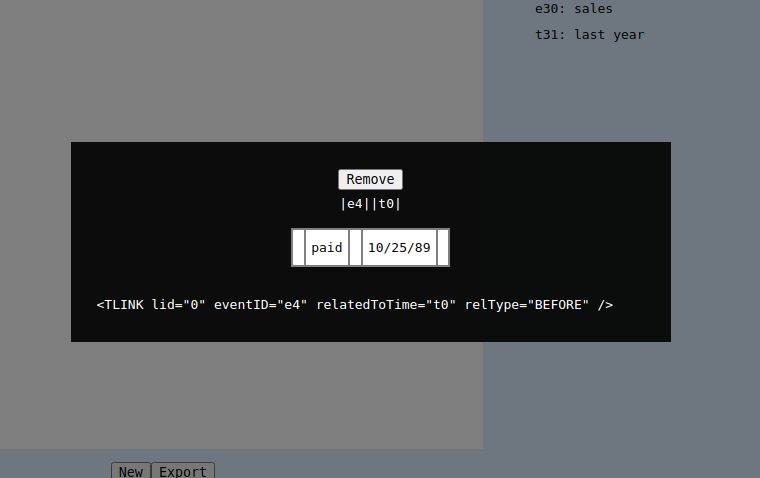
\includegraphics[width=0.8\textwidth]{images/START-clicked-string.png}
		\captionof{figure}{START: Examine a particular string.}
	\end{figure}
\end{center}
Moving over to the lower right panel, there are three drop-down menus and three buttons that become available after importing at least one event or time. If the user picks two different intervals from the drop-down menus, the `Try Find Relation' will become enabled. Clicking this will search the strings in the String bank and try to find a relation or disjunction of relations that is entailed by one or more of the strings.
\begin{center}
	\begin{figure}[h!]
		\centering
		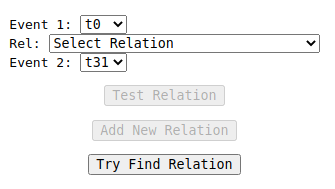
\includegraphics[width=0.4\textwidth]{images/START-try-1.png}
		\captionof{figure}{START: The relation panel.}
	\end{figure}
\end{center}
If the system finds any relations, these are reported to the user at the top of the screen. However, if no relations can be found from superposition of the strings, and both of the intervals are verbal events, then the system will attempt to make a recommendation of the relation based on the tenses and aspects of the pair of verbs, as in \citet{Derczynski2013}'s empirical validation of \citet{reichenbach1947elements}'s framework of tense and aspect. The system follows the table in \Cref{fig:tense-aspect-freksa}, p. \pageref{fig:tense-aspect-freksa}, though the suggestion will be accompanied by a warning that it \textit{is} merely a suggestion, and if one of the verbs has the event class of `REPORTING', this is highlighted to the user, since it raises the likelihood that the events are in separate temporal contexts.  If no relations can be found for the selected pair of intervals via either methodology, the user is informed of this instead.
\begin{center}
	\begin{figure}[h!]
		\centering
		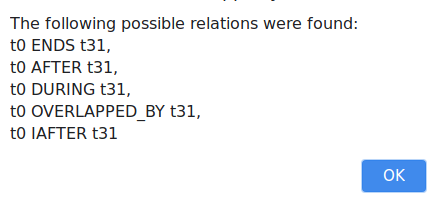
\includegraphics[width=0.4\textwidth]{images/START-try-2.png}
		\captionof{figure}{START: Relations found for a pair of intervals.}
	\end{figure}
\end{center}
If the user selects one of the relations from the drop-down list, and then clicks `Test Relation', the system will attempt to check the string(s)\footnote{The user can select an option in the `Help' menu which will allow them to choose Freksa-labelled relations in addition to the normal set as the input.} relating to that relation against the String bank. It will then inform the user with one of three statuses:
\begin{itemize}
	\item `Found': that relation already exists in the knowledge base, though it may appear in a disjunctive language, so it may be safely added to the String bank.
	\item `Possible': that relation was not found in the knowledge base, but neither was it contradicted. It may be added to the String bank.
	\item `Contradicted': A string was found that was inconsistent with that relation. It should not be added to the String bank.
\end{itemize}
\begin{center}
	\begin{figure}[h!]
		\centering
		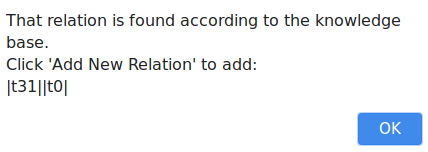
\includegraphics[width=0.4\textwidth]{images/START-test-2.png}
		\captionof{figure}{START: The result of testing a particular relation for consistency within the knowledge base.}
	\end{figure}
\end{center}
Clicking the `Add New Relation' button will, as might be expected, add a string to the String bank representing the relation that is currently specified by the drop-down menus. The full set of TimeML relations is available here, with the addition of Allen's `overlaps' and its inverse as `OVERLAPS' and `OVERLAPPED\_BY'. The primary reasoning behind including these despite their scarcity in natural language is because of the fact that they appear in a number of the disjunctions that can occur from superposition of strings.

Moving up to the top left of the screen, where the main text is, if the user moves their mouse over one of the highlighted terms, its eventID or timeID as appropriate will be indicated to help the user distinguish in case there are several highlighted elements with the same text content. The user can tag a new event by highlighting the relevant text with the mouse, and either clicking on the `Tag Event' button, or pressing the E key on their keyboard. The new event will be added to the panel on the right side of the screen, and will become available to be selected in the drop-down menus in order to relate the event to another interval. The process is the same for tagging a new time in the text, either clicking the `Tag Time' button, or pressing the T key on the keyboard after selecting some text.

Finally, moving to the panel on the right, which contains a list of all of the times and events that have been tagged in the text, if the user moves their mouse over one of the items in the list, then only the text marked up for that event or time will be highlighted in the main text area, so as to ensure the user is aware exactly which interval they are dealing with. The user can click on the `+' button to the right of the time or event to bring up another overlay containing that time or event's attributes. If the interval is not one that was imported, the attributes will be set to default values, which can be edited as needed, clicking the `Update' button to save the new values. The user can again press Escape or click outside of the panel to return to the main view. If the user clicks on the `$\times$' button, that event or time will be removed from the document, along with any strings which mention it. This is a slightly heavy-handed approach, but it is preferable to the inconsistency of being able to export a file which contains \verb|<TLINK>| tags that point to a non-existant event or time.
\begin{center}
	\begin{figure}[h!]
		\centering
		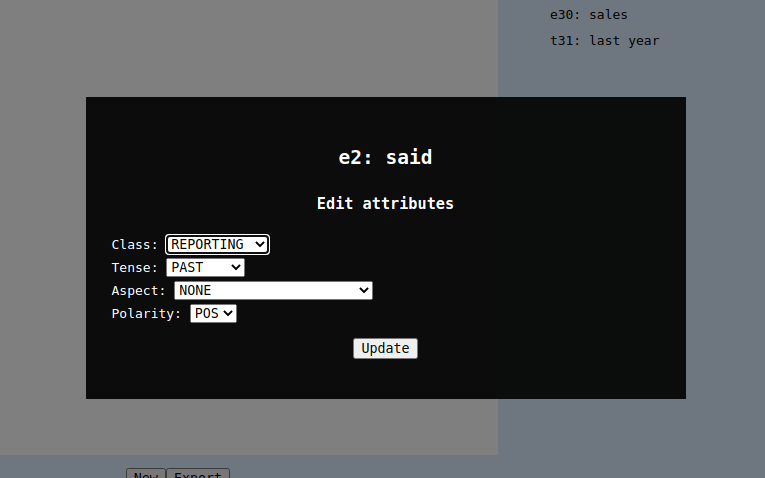
\includegraphics[width=0.8\textwidth]{images/START-event-attrs.png}
		\captionof{figure}{START: Editing some of an event's attributes.}
	\end{figure}
\end{center}
If at any point the user makes an error or wishes to go back to a previous state for some other reason, they can click the Undo button or press the U key on their keyboard to retrace their steps through their last 50 actions. This limit was chosen somewhat arbitrarily as a means to keep a handle on the memory usage in the application, though increasing the limit is unlikely to have a significant performance impact. The use can also reset the application's state at any point by clicking the `Reset' button, although this action cannot be undone, and this is effectively equivalent to refreshing the browser page.

When the user is finished with a file, they can click the `Export' button which, as mentioned, will prompt the browser to download the TimeML file. One alteration to the format of the output not already mentioned is what happens when a disjunction of relations exists in the knowledge base for some pair of intervals. Rather than exporting multiple \verb|<TLINK>| tags relating the same pair of intervals, which would instead be interpreted as the exported file containing inconsistencies, the \verb|relType| attribute of the \verb|<TLINK>| is interpreted as forming a disjunction of at least one relations, separated by the pipe character `$|$'. For example:
\begin{itemize}
	\item[\ipp] \verb!<TLINK eventID="e1" relatedToTime="t2" relType="BEFORE|IBEFORE" />!
\end{itemize}
While this does not conform with the TimeML schema, exactly, it is interpreted correctly if the exported file is re-imported back into START as a language of strings.

While this tool is not expected nor intended to compete with existing annotation tools, it does serve as a proof-of-concept of what is enabled when using the string framework to represent events and times. Superpositions can quickly find inconsistencies in a document's temporal relations, as well as generate new constraints and relations that may not have been previously explicit, while also presenting a convenient visual guide for the overall temporal structure of the annotated document. It is hoped that future work will have the opportunity to develop this tool further, and perhaps integrate it with other tooling as an alternate view alongside graphical and chart-based tools.

The next chapter examines some of the evaluation criteria for the present work, including ensuring that data cannot become lost or falsified when using the string framework.%, showing strings in use as part of a semantic test suite.%, and ensuring that the code implementing the framework is valid and behaves as expected.

\newpage
\section{Evaluation}\label{sec:evaluation}
% Evaluation is on the basis of two main components: 
In order evaluate, asserting that the string framework does not produce results that are invalid---that is, string operations do not cause contradictions internally, and they do not lose, falsify, or otherwise corrupt the original source data.%; and demonstrating the use of strings to represent the inferences which appear within the FRACAS semantic test suite.%; and verifying that the implementation code produces exactly and only the expected results.
\subsection{Timeline Validity}\label{sub:validity}
The string framework allows for compact temporal data representation with an intuitive link to timelines due to the sequential nature of the data, as explored in \cref{ssub:timelines}. However, it is crucial that these string representations do not mislead users by creating contradictory or otherwise problematic results, or if the information being operated on becomes mutated in some way that would lead to incorrect inferences being drawn that would not have been drawn before the data was manipulated. In essence, it must be ensured that when strings containing data from a source such as a document that is marked up with TimeML from the TimeBank corpus are utilised in any way, but particular after superposition as the most heavily relied upon operation in the framework, that no information becomes lost or falsified in the process.

The notion of projection---see \cref{def:projection}, p. \pageref{def:projection}---allows any given string to be tested as to whether it contains the same temporal data as some other string, which gives a way of verifying whether source material has been lost or corrupted in some way during data manipulation. It was shown in \Cref{tab:failed-projections} that the asynchronous superposition operation, which allowed for data to be combined from pairs of strings of varying lengths, did not necessarily preserve projections from its results to its sources. As a consequence, the notion of projection was built into the definition of the vocabulary-constrained superposition operation, and it was enshrined that the only valid results of the operation would be those strings which could in fact project back to the original sources.

To validate this using a concrete example, take the strings from the TimeBank document \verb|wsj_1073| again:
\begin{align}
	\{\Equals{e9}{e30}, \Before{e4}{t0}, \Before{e2}{t0}, \Before{e9}{t0}, \During{e30}{t31}\}\label{ex:validate-wsj}
\end{align}
Doing the vocabulary-constrained superposition on these strings produces a language which contains 7,449 strings.
\begin{align}
	\Equals{e9}{e30} \spvc \Before{e4}{t0} \spvc \Before{e2}{t0} \spvc \Before{e9}{t0} \spvc \During{e30}{t31}\\
	= \{ \EventString{{}|t31|e2,t31|e2,e30,e9,t31|e2,e30,e4,e9,t31|e30,e9,t31|t31|t0|{}},\label{ex:7449}\\
	\EventString{{}|e2|e2,t31|e2,e30,e9,t31|e2,e30,e4,e9,t31|e30,e9,t31|t31|t0,t31|t31|{}},\notag\\
	\EventString{{}|e2,t31|e2,e30,e9,t31|e2,e30,e4,e9,t31|e30,e9,t31|t31|t0|{}},\notag\\
	\EventString{{}|t31|e2,t31|e2,e30,e9,t31|e2,e30,e4,e9,t31|e30,e9,t31|t31|t0,t31|t0|{}},\notag\\
	\ldots \}\notag
\end{align}
Checking each string individually, every single string in \cref{ex:7449} projects to every string in \cref{ex:validate-wsj}, thus verifying that all of the original information has been preserved through the superposition to the resulting strings.

However, due to the unwieldy nature of vocabulary-constrained superposition which always performs superposition even when it sometimes doesn't make much sense from a practical point of view, the annotation tool in \cref{sec:implementation} uses instead a so-called `sensible' superposition, which avoids computing the result of superposition between strings if it is too costly to do so, based on the intersections of the inputs vocabularies and a pre-determined limit. Using this kind of superposition on \cref{ex:validate-wsj} does not in fact produce a single language, but a set of three languages, as in \cref{ex:validate-senssp}
\begin{align}
	\{\EventString{{}|t31|e30,e9,t31|t31|{}|t0|{}}, \EventString{{}|t31|e30,e9,t31|t31|t0,t31|t31|{}},\label{ex:validate-senssp}\\
	\EventString{{}|t31|e30,e9,t31|t31|t0|{}}, \EventString{{}|t31|e30,e9,t31|t31|t0,t31|t0|{}},\notag\\
	\EventString{{}|t31|e30,e9,t31|t31|t0,t31|{}}\}, \{\EventString{{}|e4|{}|t0|{}}\}, \{\EventString{{}|e2|{}|t0|{}}\}\notag
\end{align}
It's clearly not possible for every string in \cref{ex:validate-senssp} to project to every string in \cref{ex:validate-wsj}: for instance $\EventString{{}|e2|{}|t0|{}} \not\sqsupseteq \Equals{e9}{e30}$. However, sensible superposition only ever produces either strings from the vocabulary-constrained superposition or the input strings themselves, so it should be possible to find the projections, and indeed it is. The sensible superposition effectively forms a segmentation of the data, meaning that rather than each string in \cref{ex:validate-wsj} being projected to by every string in \cref{ex:validate-senssp}, every string in \cref{ex:validate-wsj} is projected to by every string in one of the languages of \cref{ex:validate-senssp}. The second and third languages contain one string each, and each projects to one string from \cref{ex:validate-wsj}. The remaining three strings \Equals{e9}{e30}, \Before{e9}{t0}, and \During{e30}{t31} are indeed all projected to by every string in the remaining (first) language of \cref{ex:validate-senssp}, thus validating that all of the information has not been lost or corrupted during superpositions.

% \subsection{FRACAS Semantic Test Suite}\label{sub:fracas}
% A de facto standard for testing semantic inferencing.
% \subsection{Correctness of Code}\label{sub:correct}
% Python test suites.
\newpage
\section{Conclusion}\label{sec:conclusion}
This thesis has described a framework for using strings as finite representations of temporal entities---times and events, as well as the relations between them. Strings have an intuitive comparison with timelines, a well-known method of conceptualising temporal information, due to their nature as sequential entities. Relevant literature was examined and discussed, in particular \citet{allen1983maintaining}'s interval algebra which forms a strong basis from which the string framework draws inspiration.

The string framework is described, including a number of operations which can be used to combine data from different strings and reason with them by inferring new temporal relations which weren't previously made explicit.

Some applications of the strings are given, in particular the use for augmenting semantic temporal annotation, for which a proof of concept tool is presented.

It is hoped that in the future this framework can be developed further and find a place among the tools of modern semantic temporal annotation.


%%%%%%%%%%%%%%%%%%%%%%%%%%%%%%%%%%%%%%%%%%%%%%%%%%%%%%%%%%%%%%%%%%%%%%%%%%%%%%%%
%                                                                              %
%                             Actual Document Ends                             %
%                                                                              %
%%%%%%%%%%%%%%%%%%%%%%%%%%%%%%%%%%%%%%%%%%%%%%%%%%%%%%%%%%%%%%%%%%%%%%%%%%%%%%%%

\newpage
\pagestyle{empty}
\onehalfspacing
\bibliographystyle{apa}
\bibliography{refs}

\newpage
%\appendix

\section*{Appendices}

\addcontentsline{toc}{section}{Appendices}
\subsection*{Python Code}
\addcontentsline{toc}{subsection}{Python Code}

\addcontentsline{toc}{subsubsection}{strfns.py}
\lstinputlisting[language=Python,breaklines=true,basicstyle=\ttfamily,title=\texttt{"""strfns.py"""}]{code/start/apiscripts/strfns.py}
\newpage
\addcontentsline{toc}{subsubsection}{freksa.py}
\lstinputlisting[language=Python,breaklines=true,basicstyle=\ttfamily,title=\texttt{"""freksa.py"""}]{code/start/api/freksa.py}
\newpage
\addcontentsline{toc}{subsubsection}{newTLINKs.py}
\lstinputlisting[language=Python,breaklines=true,basicstyle=\ttfamily,title=\texttt{"""newTLINKs.py"""}]{code/start/api/newTLINKs.py}
\newpage
\addcontentsline{toc}{subsubsection}{superpose.py}
\lstinputlisting[language=Python,breaklines=true,basicstyle=\ttfamily,title=\texttt{"""superpose.py"""}]{code/start/api/superpose.py}
\newpage
\addcontentsline{toc}{subsubsection}{test.py}
\lstinputlisting[language=Python,breaklines=true,basicstyle=\ttfamily,title=\texttt{"""test.py"""}]{code/start/api/test.py}

\newpage
\subsection*{JavaScript Code}
\addcontentsline{toc}{subsection}{JavaScript Code}

\addcontentsline{toc}{subsubsection}{index.js}
\lstinputlisting[language=Java,breaklines=true,basicstyle=\ttfamily,title=\texttt{"""index.js"""}]{code/start/pages/index.js}
\newpage
\addcontentsline{toc}{subsubsection}{parseTML.js}
\lstinputlisting[language=Java,breaklines=true,basicstyle=\ttfamily,title=\texttt{"""parseTML.js"""}]{code/start/fns/parseTML.js}
\newpage
\addcontentsline{toc}{subsubsection}{suggestTenseAspectRelation.js}
\lstinputlisting[language=Java,breaklines=true,basicstyle=\ttfamily,title=\texttt{"""suggestTenseAspectRelation.js"""}]{code/start/fns/suggestTenseAspectRelation.js}
\newpage
\addcontentsline{toc}{subsubsection}{CreateRelation.js}
\lstinputlisting[language=Java,breaklines=true,basicstyle=\ttfamily,title=\texttt{"""CreateRelation.js"""}]{code/start/components/CreateRelation.js}
\newpage
\addcontentsline{toc}{subsubsection}{Details.js}
\lstinputlisting[language=Java,breaklines=true,basicstyle=\ttfamily,title=\texttt{"""Details.js"""}]{code/start/components/Details.js}
\newpage
\addcontentsline{toc}{subsubsection}{EventList.js}
\lstinputlisting[language=Java,breaklines=true,basicstyle=\ttfamily,title=\texttt{"""EventList.js"""}]{code/start/components/EventList.js}
\newpage
\addcontentsline{toc}{subsubsection}{ExamineString.js}
\lstinputlisting[language=Java,breaklines=true,basicstyle=\ttfamily,title=\texttt{"""ExamineString.js"""}]{code/start/components/ExamineString.js}
\newpage
\addcontentsline{toc}{subsubsection}{Help.js}
\lstinputlisting[language=Java,breaklines=true,basicstyle=\ttfamily,title=\texttt{"""Help.js"""}]{code/start/components/Help.js}
\newpage
\addcontentsline{toc}{subsubsection}{StringBank.js}
\lstinputlisting[language=Java,breaklines=true,basicstyle=\ttfamily,title=\texttt{"""StringBank.js"""}]{code/start/components/StringBank.js}
\newpage
\addcontentsline{toc}{subsubsection}{TextDisplay.js}
\lstinputlisting[language=Java,breaklines=true,basicstyle=\ttfamily,title=\texttt{"""TextDisplay.js"""}]{code/start/components/TextDisplay.js}
\newpage
\addcontentsline{toc}{subsubsection}{TextEntry.js}
\lstinputlisting[language=Java,breaklines=true,basicstyle=\ttfamily,title=\texttt{"""TextEntry.js"""}]{code/start/components/TextEntry.js}


\end{document}
